\documentclass[11pt, oneside]{book}   		% Allgemeine Schriftgröße, Dokumententyp
%!TEX root=../Vorlage_DA.tex
%	%%%%%%%%%%%%%%%%%%%%%%%%%%%%%%%%%%%%%%%%%%%%%%%%%%%%%%%%
% 	Packages
%	%%%%%%%%%%%%%%%%%%%%%%%%%%%%%%%%%%%%%%%%%%%%%%%%%%%%%%%%
\usepackage{geometry}                		
\usepackage{german}
\usepackage{ngerman}
\usepackage[parfill]{parskip}    			% Activate to begin paragraphs with an empty line rather than an indent
\usepackage{graphicx}						% Use pdf, png, jpg, or epsß with pdflatex; use eps in DVI mode
											% TeX will automatically convert eps --> pdf in pdflatex		

%\usepackage{helvet}						% Kommentar wegnehmen, um in Helvetica zu schreiben
%\renewcommand{\familydefault}{\sfdefault}
%\fontfamily{phv}\selectfont
					
\usepackage{longtable}					
								
\usepackage{amssymb}
\usepackage[utf8]{inputenc}

\usepackage{multirow}
\usepackage{rotating}
\usepackage{pifont}
\usepackage{changepage}
\usepackage{wrapfig}
\usepackage{pdfpages}
\usepackage{amsmath}
\usepackage{ifthen}

\usepackage{geometry}
\usepackage{tabularx}
\usepackage{multirow}
\usepackage{arydshln}
\usepackage{subfig}
\usepackage{rotating}
\usepackage{changepage}
\usepackage{wrapfig}

\usepackage{forloop}								
\usepackage{listings}
\usepackage{color} 
% formate vertical table rows white!
% \usepackage{colortbl}
\usepackage{courier}
\usepackage{pifont}

\usepackage[pdftex]{hyperref}
\usepackage{url}

\hypersetup{
  colorlinks=true,
  linkcolor=black,
  bookmarksopenlevel=section
}

%	%%%%%%%%%%%%%%%%%%%%%%%%%%%%%%%%%%%%%%%%%%%%%%%%%%%%%%%%
% 	Dokumentabmessungen, Farbdefinitionen	
%	%%%%%%%%%%%%%%%%%%%%%%%%%%%%%%%%%%%%%%%%%%%%%%%%%%%%%%%%
%\geometry {a4paper, left=22mm, right=22mm, top=25mm, bottom=25mm, landscape}
\geometry {a4paper, bottom=30mm}%, left=30mm, right=30mm, top=25mm, bottom=25mm}
\pagestyle{headings}

\setlength{\floatsep}{7pt plus 4pt minus 4pt}
\setlength{\textfloatsep}{7pt plus 4pt minus 4pt}
\setlength{\intextsep}{7pt plus 4pt minus 4pt}

\definecolor{grey}{RGB}{127,127,127}
\definecolor{lightgrey}{RGB}{180,180,180}
\definecolor{darkgrey}{RGB}{90,90,90}
\definecolor{dkgreen}{rgb}{0,0.6,0}  
\definecolor{gray}{rgb}{0.5,0.5,0.5} 
\definecolor{mauve}{rgb}{0.58,0,0.82}

\definecolor{maroon}{rgb}{0.5,0,0}

\definecolor{cssId}{rgb}		{0,0,0.6 }%{0.75, 0.00, 0.00 }
\definecolor{cssAttribute}{rgb}	{0.58,0,0.82 }%{0.00, 0.00, 0.75 }
\definecolor{cssClass}{rgb}		{0,0,0.6 }%{0.00, 0.75, 0.00 }
\definecolor{cssComment}{rgb}	{0,0.6,0 }%{0.00, 0.75, 0.00 }
\definecolor{cssString}{rgb}	{0.6,0,0 }%{0.00, 0.75, 0.00 }

\definecolor{punct}{rgb}	{0.6,0,0 }%{0.00, 0.75, 0.00 }

\definecolor{highlight}{RGB}{255,255,204}

%	%%%%%%%%%%%%%%%%%%%%%%%%%%%%%%%%%%%%%%%%%%%%%%%%%%%%%%%%
% 	Diverse Befehle		
%	%%%%%%%%%%%%%%%%%%%%%%%%%%%%%%%%%%%%%%%%%%%%%%%%%%%%%%%%

%	Quelltext im Textfluss
\def\inlinecode#1{\texttt{\color{darkgray}{#1}}}


%	Paragraph mit Zeilenumbruch nachher
\def\htlParagraph#1{\paragraph*{#1}$\;$}
%\def\htlParagraph#1{\paragraph*{#1}$\;$ \\}

%	sub Paragraph mit Zeilenumbruch nachher
\def\subhtlParagraph#1{\textcolor{darkgrey}{\subparagraph*{#1}$\;$}}

%\def\subhtlParagraph#1{\textcolor{darkgrey}{\subparagraph*{#1}$\;$} \\}

\setcounter{secnumdepth}{3}

%	%%%%%%%%%%%%%%%%%%%%%%%%%%%%%%%%%%%%%%%%%%%%%%%%%%%%%%%%
% 	Code Formatierung		
%	%%%%%%%%%%%%%%%%%%%%%%%%%%%%%%%%%%%%%%%%%%%%%%%%%%%%%%%%
\lstset{literate=%
{Ö}{{\"O}}1 
{Ä}{{\"A}}1 
{Ü}{{\"U}}1 
{ß}{{\ss}}2 
{ü}{{\"u}}1 
{ä}{{\"a}}1 
{ö}{{\"o}}1
}
 
\lstset{ % 
%  language=Octave,                			% the language of the code 
%  basicstyle=\footnotesize,           		% the size of the fonts that are used for the code 
 	basicstyle=\ttfamily, ,           		% the size of the fonts that are used for the code 
	numbers=left,                   		% where to put the line-numbers 
	numberstyle=\tiny\color{gray},  		% the style that is used for the line-numbers 
	stepnumber=1,                   		% the step between two line-numbers. If it's 1, each line  
                                  			% will be numbered 
	numbersep=5pt,                  		% how far the line-numbers are from the code 
	backgroundcolor=\color{white},    	  	% choose the background color. You must add \usepackage{color}
	showspaces=false,               		% show spaces adding particular underscores 
	showstringspaces=false,      	   		% underline spaces within strings
	showtabs=false,                 		% show tabs within strings adding particular underscores
%	frame=single,                   		% adds a frame around the code
	frame=l,
	rulecolor=\color{dkgreen},        		% if not set, the frame-color may be changed on line-breaks within not-black text (e.g. comments (green here))
	tabsize=2,                      		% sets default tabsize to 2 spaces
	captionpos=b,                   		% sets the caption-position to bottom
	breaklines=true,                		% sets automatic line breaking
	breakatwhitespace=false,        		% sets if automatic breaks should only happen at whitespace
%	title=\lstname,                   		% show the filename of files included with \lstinputlisting;
          	                        		% also try caption instead of title
	keywordstyle=\color{blue},          	% keyword style
	commentstyle=\color{dkgreen},       	% comment style
	stringstyle=\color{mauve},    	     	% string literal style
	escapeinside={\%*}{*)},            		% if you want to add LaTeX within your code
	morekeywords={*,...},              		% if you want to add more keywords to the set
	deletekeywords={...}             	 	% if you want to delete keywords from the given language
}

%	%%%%%%%%%%%%%%%%%%%%%%%%%%%%%%%%%%%%%%%%%%%%%%%%%%%%%%%%
% 	CSS		
\lstdefinelanguage{CSS}{
		alsoletter={\\,/,*,:,-,\#,.},
		identifierstyle=\idstyle,
        keywords={accelerator:, azimuth:, background:, background-attachment:, background-color:, background-image:, background-position:, background-position-x:, background-position-y:, background-repeat:, behavior:, border:, border-bottom:, border-bottom-color:, border-bottom-style:, border-bottom-width:, border-collapse:, border-color:, border-left:, border-left-color:, border-left-style:, border-left-width:, border-right:, border-right-color:, border-right-style:, border-right-width:, border-spacing:, border-style:, border-top:, border-top-color:, border-top-style:, border-top-width:, border-width:, bottom   :, caption-side:, clear:, clip:, color:, content:, counter-increment:, counter-reset:, cue:, cue-after:, cue-before:, cursor:, direction:, display:, elevation:, empty-cells :, filter:, float:, font:, font-family:, font-size:, font-size-adjust:, font-stretch:, font-style:, font-variant:, font-weight:, height:, ime-mode:, include-source:, layer-background-color:, layer-background-image:, layout-flow:, layout-grid:, layout-grid-char:, layout-grid-char-spacing:, layout-grid-line:, layout-grid-mode:, layout-grid-type:, left:, letter-spacing:, line-break:, line-height:, list-style:, list-style-image:, list-style-position:, list-style-type:, margin:, margin-bottom:, margin-left:, margin-right:, margin-top:, marker-offset:, marks:, max-height:, max-width:, min-height:, min-width:, -moz-binding:, -moz-border-radius:, -moz-border-radius-topleft:, -moz-border-radius-topright:, -moz-border-radius-bottomright:, -moz-border-radius-bottomleft:, -moz-border-top-colors:, -moz-border-right-colors:, -moz-border-bottom-colors:, -moz-border-left-colors:, -moz-opacity:, -moz-outline:, -moz-outline-color:, -moz-outline-style:, -moz-outline-width:, -moz-user-focus:, -moz-user-input:, -moz-user-modify:, -moz-user-select:, orphans:, outline:, outline-color:, outline-style:, outline-width:, overflow:, overflow-X:, overflow-Y:, padding:, padding-bottom:, padding-left:, padding-right:, padding-top:, page:, page-break-after:, page-break-before:, page-break-inside:, pause:, pause-after:, pause-before:, pitch:, pitch-range:, play-during:, position:, quotes:, -replace:, richness:, right:, ruby-align:, ruby-overhang:, ruby-position:, -set-link-source:, size:, speak:, speak-header:, speak-numeral:, speak-punctuation:, speech-rate:, stress:, scrollbar-arrow-color:, scrollbar-base-color:, scrollbar-dark-shadow-color:, scrollbar-face-color:, scrollbar-highlight-color:, scrollbar-shadow-color:, scrollbar-3d-light-color:, scrollbar-track-color :, table-layout:, text-align:, text-align-last:, text-decoration:, text-indent:, text-justify:, text-overflow:, text-shadow:, text-transform:, text-autospace:, text-kashida-space:, text-underline-position:, top:, unicode-bidi:, -use-link-source:, vertical-align:, visibility:, voice-family:, volume :, white-space:, widows:, width:, word-break:, word-spacing:, word-wrap:, writing-mode},
        keywordstyle=\color{cssAttribute},%\bfseries,
        ndkeywords={@import, @media, @page, @font-face, @charset, @namespace, a, html, body, title, pre, h1, h2, h3, h4, h5, h6, ul, ol, li, p, br, blockquote, dl, dt, dd, div, img, strong, em, cite, tt, i, b, table, tr, td, th, frame, form, option, input, button, nav, section, article, aside, footer, hr, sup, sub, del, ins, small, span},
        ndkeywordstyle=\color{cssId},%,\bfseries,
%        identifierstyle=\color{black},
%        sensitive=false,
%        comment=[l]{//},
        morecomment=[s]{/*}{*/},
        commentstyle=\color{cssComment}\ttfamily,
        stringstyle=\color{cssString}\ttfamily,
        morestring=[b]',
        morestring=[b]"
}

\makeatletter
\newcommand*\idstyle[1]{%
         \expandafter\id@style\the\lst@token{#1}\relax%
 }

 \def\id@style#1#2\relax{%
           	\ifnum\pdfstrcmp{#1}{\#}=0%
                \small\ttfamily\color{cssId} \the\lst@token%
            \else%
		      	\ifnum\pdfstrcmp{#1}{.}=0%
    	            \small\ttfamily\color{cssClass} \the\lst@token%
        		\else%
					\ifnum\pdfstrcmp{#1}{:}=0%
    	            	\small\ttfamily\color{cssAttribute} \the\lst@token%
        			\else%
		     	 		\edef\tempa{\uccode`#1}%
              			\edef\tempb{`#1}%
              			\ifnum\tempa=\tempb%
                			\small\ttfamily\color{mauve} \the\lst@token%
              			\else%
                 	 		\the\lst@token%
    	         		\fi%
	           		\fi%
	            \fi%
            \fi%
 }
\makeatother

%	%%%%%%%%%%%%%%%%%%%%%%%%%%%%%%%%%%%%%%%%%%%%%%%%%%%%%%%%
% 	C Compact
\lstdefinelanguage{CMM}{
        keywords={bool, int, float, char, string, library, wait},
		alsoletter={\{,\}\\,/,*,:,-,\#,.},
        comment=[l]{//},
        morecomment=[s]{/*}{*/},
        morestring=[b]',
        morestring=[b]"
}

%	%%%%%%%%%%%%%%%%%%%%%%%%%%%%%%%%%%%%%%%%%%%%%%%%%%%%%%%%
% 	EBNF	
\lstdefinelanguage{EBNF}{
        keywords={},
		alsoletter={\{,\}\\,/,*,:,-,\#,.},
        comment=[l]{//},
        morecomment=[s]{/*}{*/},
        morestring=[b]',
        morestring=[b]",
        literate={.}{{\textcolor{punct}{.}}}{1}
				{)}{{\textcolor{punct}{)}}}{1}		% not working!
				{(}{{\textcolor{punct}{(}}}{1}
				{\{}{{\textcolor{punct}{\{}}}{1}
				{\}}{{\textcolor{punct}{\}}}}{1}
				{=}{{\textcolor{punct}{=}}}{1}
				{<}{{\textcolor{punct}{<}}}{1}
				{>}{{\textcolor{punct}{>}}}{1}
}
%	%%%%%%%%%%%%%%%%%%%%%%%%%%%%%%%%%%%%%%%%%%%%%%%%%%%%%%%%
% 	XML
\lstdefinelanguage{XML}
{
  basicstyle=\ttfamily\footnotesize,
  morestring=[b]",
  moredelim=[s][\bfseries\color{maroon}]{<}{\ },
  moredelim=[s][\bfseries\color{maroon}]{</}{>},
  moredelim=[l][\bfseries\color{maroon}]{/>},
  moredelim=[l][\bfseries\color{maroon}]{>},
  morecomment=[s]{<?}{?>},
  morecomment=[s]{<!--}{-->},
%  commentstyle=\color{DarkOliveGreen},
%  stringstyle=\color{blue},
  identifierstyle=\color{red}
}		% Formatierung der Dokuments, Diverse Befehle

%	########################################################
% 					Autoren		
%	########################################################
\newboolean{fabian}
\newboolean{thomas}
\newboolean{peter}

\setboolean{fabian}{true}
\setboolean{thomas}{true}
\setboolean{peter}{true}

%	########################################################
% 					Allgemeine Informationen			
%	########################################################
\def\htlArbeit{Diplomarbeit }
\def\htlArbeitsthema{C Compact }	% Thema oder Titel der Arbeit
\def\htlArbeitstitel{C Compact }			% Arbeitstitel

%\lstset{basicstyle=\small}


\begin{document}

%	########################################################
% 						Einleitung			
%	########################################################
\pagenumbering{roman}	% Beginn mit römischen Seitenzahlen

%	--------------------------------------------------------
% 	Deckblatt
%	--------------------------------------------------------			
%
\input{./chapters/Pre-01-deckblatt.tex}

%	--------------------------------------------------------
% 	Arbeitstitel
%	--------------------------------------------------------		
%!TEX root=../Vorlage_DA.tex
%	########################################################
% 							Arbeitstitel
%	########################################################


%	--------------------------------------------------------
% 	Überschrift, Inhaltsverzeichnis
%	--------------------------------------------------------
\chapter*{Arbeitstitel: \newline \htlArbeitstitel}



%	--------------------------------------------------------
% 	Bearbeiter
%	--------------------------------------------------------
\htlParagraph{Bearbeiter:}
\iffabian \\Fabian Hummer \fi \ifthomas \\Thomas Pointhuber  \fi \ifpeter \\ Peter Wassermair \fi


%	--------------------------------------------------------
% 	Beteiligte Firmen
%	--------------------------------------------------------
\htlParagraph{An der \htlArbeit beteiligte Firmen:}

\renewcommand{\arraystretch}{1.5}
\begin{tabularx}{1\textwidth}{@{} l X @{}}

\emph{Firma:} & Institut für Systemsoftware\newline Johannes Kepler Universität Linz\\
\emph{Adresse:} & Altenbergstraße, 69\\
\emph{Plz, Ort:} & 4040, Linz\\
\emph{Kontaktperson:} & Prof. Dr. Dr. h.c. Hanspeter Mössenböck\\
\emph{Telefon:} & + 43-732-2468-4340\\
\emph{E-Mail:} & moessenboeck@ssw.uni-linz.at\\

\end{tabularx}


%	--------------------------------------------------------
% 	Eidesstattliche Erklärung
%	--------------------------------------------------------			
%!TEX root=../Vorlage_DA.tex
%	########################################################
% 					Eidesstattliche Erklärung
%	########################################################


%	--------------------------------------------------------
% 	Überschrift, Inhaltsverzeichnis
%	--------------------------------------------------------
\chapter*{Erklärung}
\addcontentsline{toc}{chapter}{Erklärung}


%	--------------------------------------------------------
% 	Inhalt
%	--------------------------------------------------------

Ich erkläre an Eides statt, dass ich die vorliegende Diplomarbeit selbstständig und ohne fremde Hilfe verfasst, andere als angegebene Quellen und Hilfsmittel nicht direkt benutzt und die benutzten Quellen wörtlich und inhaltlich entnommenen Stellen als solche erkenntlich gemacht habe.
\vspace{3cm}

\iffabian
\begin{tabularx}{1\textwidth}{X p{1cm} X p{1cm} X}
\hrulefill & & \hrulefill & & \hrulefill \\
\emph{Ort, Datum} & & \emph{Verfasser Vor- und Zunamen} & & \emph{Unterschrift}
\end{tabularx}
\fi



\ifthomas
\begin{tabularx}{1\textwidth}{X p{1cm} X p{1cm} X}
\hrulefill & & \hrulefill & & \hrulefill \\
\emph{Ort, Datum} & & \emph{Verfasser Vor- und Zunamen} & & \emph{Unterschrift}
\end{tabularx}
\fi

\ifpeter
\begin{tabularx}{1\textwidth}{X p{1cm} X p{1cm} X}
\hrulefill & & \hrulefill & & \hrulefill \\
\emph{Ort, Datum} & & \emph{Verfasser Vor- und Zunamen} & & \emph{Unterschrift}
\end{tabularx}
\fi




%	--------------------------------------------------------
% 	Vorwort
%	--------------------------------------------------------	
%!TEX root=../Vorlage_DA.tex
%	########################################################
% 							Vorwort
%	########################################################


%	--------------------------------------------------------
% 	Überschrift, Inhaltsverzeichnis
%	--------------------------------------------------------
\chapter*{Vorwort}
\addcontentsline{toc}{chapter}{Vorwort}


%	--------------------------------------------------------
% 	Inhalt
%	--------------------------------------------------------

Wir möchten uns bei unseren Projektbetreuern am Institut für Systemsoftware der Johannes Kepler Universität Linz bedanken, die uns bei unserem Praktikum zu Beginn des Projektes und während des Jahres unterstützt haben. Wir konnten einen interessanten Einblick in den Alltag und die Arbeitsweise an der Universität erhalten.

Besonderer Dank gilt unserem Projektbetreuer, Herrn Matejka, der uns während des Projektes stets mit Rat und Tat zur Seite gestanden ist und uns mit seiner Erfahrung als Lehrer einen anderen Blickwinkel auf die Entwicklung von C Compact eingebracht hat.

Einen wertvollen Beitrag haben die Schülerinnen und Schüler geleistet, die bei den Versuchen beteiligt waren und uns somit laufend auf die Schwächen und Probleme unserer Entwicklungsumgebung aufmerksam gemacht, uns aber auch das Potential und die Vorteile von C Compact gezeigt haben.

Schließlich möchten wir noch den Lehrern danken, die uns jeweils mehrere Unterrichtsstunden zur Verfügung gestellt haben, um diese Tests zu ermöglichen.

Wir hoffen, dass C Compact seine Anwendung im Unterricht nicht nur während dieser Versuche gefunden hat. Die Schülerinnen und Schüler konnten von von den Features und der anschaulichen Oberfläche von C Compact profitieren und gaben uns durchwegs positive Rückmeldungen. Damit C Compact jederzeit und von jedem verwendet werden kann, haben wir beschlossen, diese Entwicklungsumgebung unter der GNU General Public License öffentlich zur Verfügung zu stellen.

%	--------------------------------------------------------
% 	Zusammenfassung
%	--------------------------------------------------------		 	  
%!TEX root=../Vorlage_DA.tex
%	########################################################
% 							Zusammenfassung
%	########################################################


%	--------------------------------------------------------
% 	Überschrift, Inhaltsverzeichnis
%	--------------------------------------------------------
\chapter*{Zusammenfassung}
\addcontentsline{toc}{chapter}{Zusammenfassung}



%	--------------------------------------------------------
% 	Inhalt
%	--------------------------------------------------------

C Compact ist eine Entwicklungsumgebung, die besonders auf die Bedürfnisse von angehenden Programmierern ausgelegt ist. Diese Umgebung sollte vor allem in den ersten und zweiten Klassen der HTL Anwendung finden, wo Schülerinnen und Schüler erste und oft schwierige Erfahrungen mit dem Programmieren machen. Während professionelle Entwicklungsumgebungen einen oftmals unübersichtlich breiten Funktionsumfang haben, setzt C Compact auf intuitive und einfache Bedienung.

Die Schüler arbeiten dabei mit einer Sprache, die C sehr ähnlich ist.
Trotz des äußerlich simplen Aufbaus liefert sie jedoch den vollen Umfang einer anspruchsvollen Programmiersprache und den damit verbundenen Programmiertechniken. C Compact ist sowohl zum Lösen einfacher Aufgaben, als auch zum Entwickeln komplexer Algorithmen geeignet und kann bis in die dritte Klasse verwendet werden.

Die Entwicklungsumgebung enthält einen integrierten Debugger, der von Anfang an ein fundiertes Verständnis für die Logik und den Ablauf eines Computerprogramms vermitteln soll. Viele Irrtümer und Verständnisprobleme können bereits durch grafische Veranschaulichungen ausgeschlossen werden. Tritt ein Fehler im Quelltext auf, erhält der Benutzer eine leicht verständliche Fehlerbeschreibung und Hinweise zum Suchen der Fehlerstelle.



%	--------------------------------------------------------
% 	Abstract
%	--------------------------------------------------------		
%!TEX root=../Vorlage_DA.tex
%	########################################################
% 							Abstract
%	########################################################


%	--------------------------------------------------------
% 	Überschrift, Inhaltsverzeichnis
%	--------------------------------------------------------
\chapter*{Abstract}
\addcontentsline{toc}{chapter}{Abstract}



%	--------------------------------------------------------
% 	Inhalt
%	--------------------------------------------------------
C Compact is a simple but powerful development environment for a programming language similar to C. It is especially adjusted to the needs of programming beginners who often have troubles understanding the way a program works and the logic it is based on.

In contrast to professional IDEs, C Compact can be used easily and in an intuitive way. However, it also provides the full range of features that are needed for programming lessons at technical schools. C Compact can be used to aquire simple tasks as well as to develop complex algorithms.

This IDE is intended for the use in programming lessons in the first two grades of Austrian technical colleges (HTL). Though, C Compact is not limited to this application. It can also be used for advanced training or programming courses as well as by hobby programmers.

C Compact is distributed under the terms of GNU General Public License and is therefore free software. 

%	--------------------------------------------------------
% 	Inhaltsverzeichnis
%	--------------------------------------------------------			
\tableofcontents



%	########################################################
% 						Arbeit			
%	########################################################

%	--------------------------------------------------------
% 	INFO: Zitieren, Abbildungen, Listing
%	-------------------------------------------------------	
%\input{./chapters/Pre-XX-beispiele.tex} 	% Nur zur Info

%	--------------------------------------------------------
% 	Aufgabenstellung / Pflichtenheft
%	--------------------------------------------------------		
%\input{./chapters/01-aufgabenstellung.tex}
\pagenumbering{arabic}	% Beginn mit arabischen Seitenzahlen

% Einleitung
\iffabian
	%!TEX root = "../../DA_GUI.tex"

\chapter{Einleitung}

\section{Die Projektidee}
Für Firmen ist es schwierig, gut ausgebildete Programmierer zu finden, eine Reihe von Stellen bleiben unbesetzt. Etliche Firmen werden dadurch daran gehindert, zu expandieren oder wichtige Aufträge anzunehmen.
Ein wesentlicher Grund für diese Misere ist, dass das Erlernen einer Programmiersprache eine anspruchsvolle Tätigkeit ist. Besonders Anfänger stoßen oft auf Schwierigkeiten.

Im Rahmen des Projektes C Compact wurde eine speziell für die Ausbildung konzipierte Entwicklungsumgebung erarbeitet. Diese soll den Einstieg in C durch intuitive Bedienung und anschauliche Darstellung von Programmabläufen erleichtern.

\section{Projektorganisation}

Das Projekt C Compact wurde in Zusammenarbeit mit dem Institut für Systemsoftware\footnote{http://ssw.jku.at/} der Johannes Kepler Universität Linz durchgeführt. Jeder Projektschüler ist für einen Bereich des Projektes verantwortlich und wird dabei von einem Projektbetreuer der Universität unterstützt. Das Diplomprojekt selbst wird von Herrn Dipl.Ing. Franz Matejka betreut. Tabelle \ref{tab:intro-work-1} zeigt die Aufgabenverteilung, wie sie zu Beginn des Projektes festgelegt wurde.

\def\arraystretch{1.4}
\begin{table}
\begin{tabular}{|l|l|l|}
\hline
\textbf{Projektschüler}&\textbf{Projektbetreuer}&\textbf{Aufgabenbereich}\\
\hline
Thomas Pointhuber & Univ.Prof. Hanspeter Mössenböck & Compiler \\
Peter Wassermair & Dipl.Ing. Matthias Grimmer & Interpreter \\
Fabian Hummer & Univ.Prof. Günther Blaschek & Benutzeroberfläche\\
\hline
\end{tabular}
\caption{Ursprüngliche Aufgabeneinteilung}
\label{tab:intro-work-1}
\end{table}

\section{Terminübersicht}

Der Großteil der Projektarbeit wurde als Freizeitleistung durchgeführt. Eine genaue Aufstellung der Arbeitszeiten ist in Anhang \ref{projekttagebuch} zu finden.

Die Entwicklung von C Compact wurde in den Sommerferien 2014 --- in Form eines Praktikums der Projektschüler am Institut für Systemsoftware --- begonnen. Bereits im Vorfeld wurden einige Projektanforderungen festgelegt (siehe Kapitel \ref{sec:intro.anf}). Das Praktikum begann am 7. Juli 2014 und dauerte 2 bzw. 4 Wochen\footnote{Praktikum an der JKU von 7.7.2014 bis 18.7.2014, bzw. Peter Wassermair von 7.7.2014 bis 1.8.2014}. Wir erlernten zu Beginn die Grundlagen und Techniken von Compiler und Interpreter und konnten schnell mit der Entwicklung starten.

Am 22. Dezember 2014 wurde den Projektbetreuern an der JKU der Projektfortschritt vorgestellt, daraufhin wurden weitere Entwicklungsschritte zum Questsystem und zum Compiler besprochen.

Eine abschließende Besprechung am Institut für Systemsoftware ist für Juni 2015 vorgesehen.

Im Laufe des Schuljahres wurde C Compact mit unterschiedlichen Funktionen und Bestandteilen erweitert. Tabelle \ref{tab:intro-milestones} zeigt eine grobe Einteilung der Projektarbeit in einzelne Meilensteine.

\begin{table}[h!]
\def\arraystretch{1.6}
\begin{tabularx}{\columnwidth}{|l|XXX|}
\hline
  \textbf{Zeitraum}&\textbf{Thomas Pointhuber}&\textbf{Peter Wassermair}&\textbf{Fabian Hummer}\\
  \hline
  Sommerferien 2014\footnote{Praktikum an der JKU von 7.7.2014 bis 18.7.2014, bzw. Peter Wassermair von 7.7.2014 bis 1.8.2014} & Compiler & Interpreter & Benutzeroberfläche, Entwicklugnsumgebung \\
  Sept. - Dez. 2014 & Implementierung weiterer Sprachfunktionen & Grundgerüst des Aufgabensystens, Dateistruktur & Verbesserung der Benutzeroberfläche, Versuche mit Schülergruppen \\
  Januar - März 2015 & Testen und Dokumentieren von Sprachfunktionen & Integration des Aufgabensystems in die Entwicklungsumgebung & Abschließen der Entwicklungsumgebung, Hilfe bei Questsystem\\
  April - Mai 2015 & \multicolumn{3}{c}{Fehlerbehebung, kleine Erweiterungen und Dokumentation}\\
  \hline
\end{tabularx}
\caption{Meilensteine in der Entwicklung von C Compact}
\label{tab:intro-milestones}
\end{table}


\section{C Compact im Überblick}

\subsection*{Die Sprache}
Die Benutzer arbeiten bei C Compact mit einer Programmiersprache, die C sehr ähnlich ist. Trotz des äußerlich simplen Aufbaus kann sie den vollen Umfang einer anspruchsvollen Programmiersprache und die damit verbundenen Programmiertechniken vermitteln.

Bekannte C-Bibliotheken wie \glqq{}stdlib.h\grqq{}sind in C Compact ebenfalls vorhanden, um auch komplexere Programme einfach umsetzen zu können. Außerdem wurde ein einfacher Präprozessor implementiert, um Projekte mit mehreren Dateien zu ermöglichen.

\subsection*{Die Umgebung}
Viele Irrtümer und Verständnisprobleme, die bei angehenden Programmierern immer wieder auftreten, sollen bereits durch die Entwicklungsumgebung selbst ausgeschlossen werden. Deshalb ist die Benutzeroberfläche ein essenzieller Bereich von C Compact. %Wir haben häufig auftretende Missverständnisse und Denkfehler analysiert und Features erarbeitet, die eben jene Probleme ausschließen sollen.


\begin{figure}[h!]
	\centering
	\includegraphics[width=0.7\textwidth]{./media/images/gui/main/CCompactAlpha1-4-5-guimain.png}
	\caption{Die Benutzeroberfläche von C Compact}
	\label{fig:intro-over-gui}
\end{figure}

Ein wichtiger Bestandteil der Benutzeroberfläche ist der integrierte Debugger (in Abbildung \ref{fig:intro-over-gui} rechts), der speziell für die Bedürfnisse von Anfängern ausgelegt ist. Während das Programm Schritt für Schritt abgearbeitet wird, sind alle Variablen und der Call Stack in übersichtlicher Form dargestellt. In der Variablentabelle werden Wertänderungen farbig hervorgehoben. Dadurch soll ein fundiertes Verständnis für den Programmablauf und die Logik dahinter entstehen.
Ein weiterer daraus resultierender Vorteil ist, dass Schüler von Anfang an mit einem Debugger arbeiten und ähnliche Tools später auch in anderen Entwicklungsumgebungen verwenden werden. Der Debugger wird in Kapitel \ref{sec:deb} beschrieben.

Um sicherzustellen, dass die Entwicklungsumgebung wirkungsvoll ist und zuverlässig funktioniert, wurde sie regelmäßig mit Gruppen der zweiten Klassen der HTL Braunau getestet. Bei diesen Versuchen lösten die Schülerinnen und Schüler komplexe Aufgaben mithilfe von C Compact und bewerten Benutzerfreundlichkeit und Bedienbarkeit nachher in einem Fragebogen. Siehe Kapitel \ref{sec:sci-trial-intro}.

\subsection*{Integration im Unterricht}
Um den Programmierunterricht zu verbessern und effektiver zu gestalten, wurde auf aktuellen und bewährten Unterrichtsmethoden aufgebaut werden. C Compact soll Lehrer wie Schüler unterstützen. Zu diesem Zweck wurden einige FSST-Lehrer (Fachspezifische Softwaretechnik) unserer Schule zum Aufbau und Ablauf ihrer Stunden befragt, um Einsatzmöglichkeiten für C Compact zu erkennen. Gewonnene Erkenntnisse flossen laufend in den Entwicklungsprozess von C Compact ein. Siehe Kapitel \ref{sec:sci-interview}.

C Compact enthält außerdem ein Aufgaben- und Belohnungssystem (auch genannt Questsystem). Mit diesem System können Schüler kleine und größere Aufgaben, die in Themenblöcke gegliedert sind, lösen. Eine ausgewählte Aufgabe wird bei der Fertigstellung automatisch auf Richtigkeit überprüft. Durch den individuellen Fortschritt soll selbstständiges Lernen gefördert werden. Um kleine Erfolgserlebnisse zu vermitteln, erhalten die Benutzer für gelöste Aufgaben Auszeichnungen. Siehe Kapitel \ref{sec:quest}.

\subsection*{Verwendung und Erhältlichkeit}
Unseren Recherchen zufolge gibt es derzeit keine vergleichbare Entwicklungsumgebung für die Ausbildung. Projekte mit ähnlichen Zielen besitzen oft einen rein spielerischen Charakter oder unterstützen nur einen sehr grundlegenden Befehlssatz. In C Compact dagegen ist es möglich, komplexere Algorithmen zu entwickeln, zu visualisieren, und diese auch in späteren Projekten einzusetzen.

Wir hoffen zwar, dass C Compact vor Allem im Unterricht Verwendung findet, sind aber auch für viele andere Anwendungsbereiche offen, wie etwa bei Kursen und Schulungen oder für Hobbyprogrammierer. Deshalb haben wir beschlossen, C Compact unter der GNU General Public License\footnote{http://www.gnu.org/copyleft/gpl.html} öffentlich zur Verfügung zu stellen. Das gesamte Projekt kann auf GitHub\footnote{https://github.com/Projekt-CMM/CMM} angesehen werden.

\begin{figure}[h!]
	\centering
	
\includegraphics[width=0.3\textwidth]{./media/images/intro/GPLv3-Logo.png}
	\caption{Logo der GNU General Public License}
\end{figure}

\section{Anforderungen an C Compact}
\label{sec:intro.anf}
Für die Anwendung im Unterricht und insbesondere für die Anwendung von unerfahrenen Programmierern muss die Entwicklungsumgebung C Compact einige besondere Eigenschaften aufweisen. Die Anforderungen an diese Entwicklungsumgebung unterscheiden sich von den Anforderungen an professionelle Tools.

Die Anforderungen für die erste Version von C Compact --- die bereits im Sommer 2014 entwickelt wurde --- wurden von den Projektbetreuern an der JKU gestellt. Herr Professor Mössenböck erstellte ein Anforderungsdokument für Compiler und Interpreter, das im Laufe des Projektes erweitert wurde (siehe Anhang \ref{app:anf-comp}). Herr Professor Blaschek definierte vor Projektbeginn die grundlegenden Anforderungen an die Benutzeroberfläche von C Compact und legte ihren grundlegenden Aufbau fest (siehe Anhang \ref{app:anf-gui}). Im Laufe des Projektes wurde die Benutzeroberfläche ausgebaut.

\subsection*{Anforderungen an das Programm an sich}
Für die Anwendung im Unterricht --- insbesondere als Hilfestellung für unerfahrene Benutzer --- sind folgende Punkte besonders wichtig:
\begin{itemize}
\item \textbf{Das Programm soll auf möglichst vielen Betriebssystemen funktionieren}\\
Läuft ohne Probleme auf Windows 7, Windows 8, Mac OSX, Ubuntu 14.04, Ubuntu 14.10, Linux Mint 17.1\\
Leichte Probleme auf Windows 10 (Technical Preview)
\item \textbf{Das Programm soll einfach zu installieren sein}\\
Eine Installation ist nicht erforderlich.
\item \textbf{Das Programm soll einfach erhältlich sein}\\
C Compact ist freie Software und kann kostenlos heruntergeladen werden.
\end{itemize}

\subsection*{Anforderungen an den Compiler und den Interpreter}
Compiler und Interpreter sind grundlegende Bausteine von C Compact. Hier sind besonders Stabilität und Effizienz gefragt.
\begin{itemize}
\item \textbf{Der Compiler muss stabil laufen}\\
Durch ausführiche Tests wurden sehr viele Fehler behoben. Der Compiler läuft praktisch ohne Probleme.
\item \textbf{Die verwendete Sprache soll C möglichst ähnlich sein}\\
Es gibt leichte Unterschiede zu C, auf die im Unterricht eventuell hingewiesen werden muss. Einige der Änderungen bringen aber auch Voreteile mit sich.
\item \textbf{Die verwendete Sprache soll gegenüber C keine wesentlichen Einschränkungen enthalten}\\
C Compact kann bis in die dritte Klasse problemlos verwendet werden. Nur bei einigen sehr fortgeschrittenen Themen muss auf professionelle Compiler zurückgegriffen werden.
\end{itemize}

\subsection*{Anforderungen an die Benutzeroberfläche}
Die Benutzeroberfläche ist die Schnittstelle zwischen Mensch und Maschine. Um Programmieranfänger nicht zu überfordern, muss die Oberfläche möglichst einfach und intuitiv zu bedienen sein.
\begin{itemize}
\item \textbf{C Comapct muss einfach zu Bedienen sein}\\
Durch eine Reihe von Versuchen mit Schülerinnen und Schülern der ersten und zweiten Klassen konnten wir die Benutzeroberfläche immer wieder optimieren, sodass C Compact nun sehr übersichtlich und angenehm zu Bedienen ist.
\item \textbf{C Compact soll den Schülerinnen und Schülern helfen, Programmabläufe besser zu verstehen}\\
Der intuitiv zu bedienende Debugger von C Compact zeigt den Ablauf und die Logik eines Programms sehr anschaulich. In unseren Versuchen haben wir herausgefunden, dass C Compact tatsächlich eine Verbesserung des FSST-Unterrichts darstellt.
\item \textbf{Die Fehlermeldungen des Compilers müssen verständlich und ersichtlich sein}\\
Wenn ein Fehler auftritt erhält der Benutzer sowohl eine Angabe, wo der Fehler aufgetreten ist, als auch eine ausführliche Beschreibung des Fehlers und möglicher Fehlerursachen.
\end{itemize}

\subsection*{Anforderungen an das Questsystem}
Mit dem Questsystem können die Schülerinnen und Schüler Probleme zu einem bestimmten Thema selbstständig erarbeiten. Die Schülerinnen und Schüler lösen Aufgaben, die von C Compact gestellt werden. Das Programm überprüft auch, ob die Lösungen der Schülerinnen und Schüler korrekt ist. Für korrekte Lösungen werden Auszeichnungen vergeben.
\begin{itemize}
\item \textbf{Aufgaben müssen in Themenbereiche strukturierbar sein}\\
Aufgaben sind in beliebig viele Pakete und Bereiche --- auch mit mehreren Ebenen --- strukturierbar. Lehrer können Aufgabensammlunglen erstellen, die an ihren Unterricht angepasst sind
\item \textbf{Die Aufgaben sollten eine Verbesserung für den Unterricht darstellen}\\
Bei einem Versuch mit einer Gruppe der 1AHLES hat sich gezeigt, dass die Schüler gerne Aufgaben aus dem Questsystem erarbeiten. Durch Auszeichnungen und Anzeige des Fortschritts in einem bestimmten Themenbereich können die Schüler gezielt motiviert werden.
\end{itemize}
\fi

% Compiler
\ifthomas
	\input{./chapters/compiler/compiler.tex}
\fi

% Interpreter
\ifpeter
	%!TEX root=../Vorlage_DA.tex
%	########################################################
% 				Projektbeschreibung
%	########################################################


%	--------------------------------------------------------
% 	Überschrift, Inhaltsverzeichnis
%	--------------------------------------------------------
\chapter{Interpreter}

\section{Einführung}

%\htlParagraph{Bytecode Interpreter:}\\
%Bei der Kompilierung wird eine Zwischensprache erzeugt, welche aus einer Sammlung von Befehlen besteht. Dadurch wird das System betriebssystemunabhängig und der Code ist nahezu hardwareunabhängig.

%Jedoch muss zum Ausführen des Programmes, welches in die Zwischensprache übersetzt wurde, eine virtuelle Maschine vorhanden sein.
%Dadurch, dass während der Ausführung des Programmes compiliert werden muss, sinkt die Geschwindigkeit gegenüber nativ compilierten Programmen.

%Durch die Verwendung des Just-in-time-compilation Verfahrens kann die Geschwindigkeit wieder verbessert werden.

\htlParagraph{Abstrakter Syntaxbaum Interpreter}\\
Ein Programm muss in einer konkreten Syntax geschrieben werden. Diese Syntax ist jedoch nur für den Menschen, sie kann nicht einfach vom Computer übernommen werden. Damit der Interpreter verstehen kann, was mit einem vom Benutzer geschriebenen Programm ausdrückt werden soll, muss dieses zuerst in einen Abstrakten Syntax Baum\footnote{\url{http://de.wikipedia.org/wiki/Abstrakter_Syntaxbaum}} umgewandelt werden. Diese Umwandlung geschieht beim Parser\ref{kap:Parser}.

Nun kommt der Interpreter zum Einsatz. Er liest dem vom Parser erzeugten Code ein und arbeitet diesen zeilenweise ab. Der Interpreter, kann somit nur funktionieren, wenn der Abstrakte Syntax Baum korrekt erstellt wurde. Der Interpreter erzeugt hierbei keinen Maschinencode.

\htlParagraph{Aufbau eines Interpreters:}\\
Um eine Programmiersprache zu erstellen sind mehrere Punkte zu beachten. Zuerst sollte, eine konkrete Syntax und der Abstrakte Syntax Baum definiert werden. Nun kann ein geeignetes Memory System (Kapitel \ref{sec:memory_system}) gewählt werden. Schlussendlich, muss die Abarbeitung des Abstrakten Syntax Baumes überlegt werden.

\section{Aufbau unseres Abstrakten Syntax Baumes}
Der Abstrakte Syntax Baum wird vom Parser generiert und hat einen definierten Aufbau. Er besteht jeweils aus Knoten, welche einen Linken und einen Rechten, beziehungsweise einen weiterführenden Knoten besitzen. Die Knoten haben wiederum eine definierte Reihenfolge in welcher sie auftreten können. 

\subsection{Statements}
Statment-Knoten sind grundsätzlich immer Anweisungen. Somit können von diesem Knotentypen aus Zuweisungen, Unterprogrammaufrufe, Schleifen und If- Abfragen getätigt werden. Auch wird hier, bei Schließung eines Unterprogramms der nötige "`return"' oder bei einer Funktion mit fehlenden Rückgabewert ein "`trap"' Knoten aufgerufen.

%TODO PDF
\begin{figure}[h] 
  \centering
     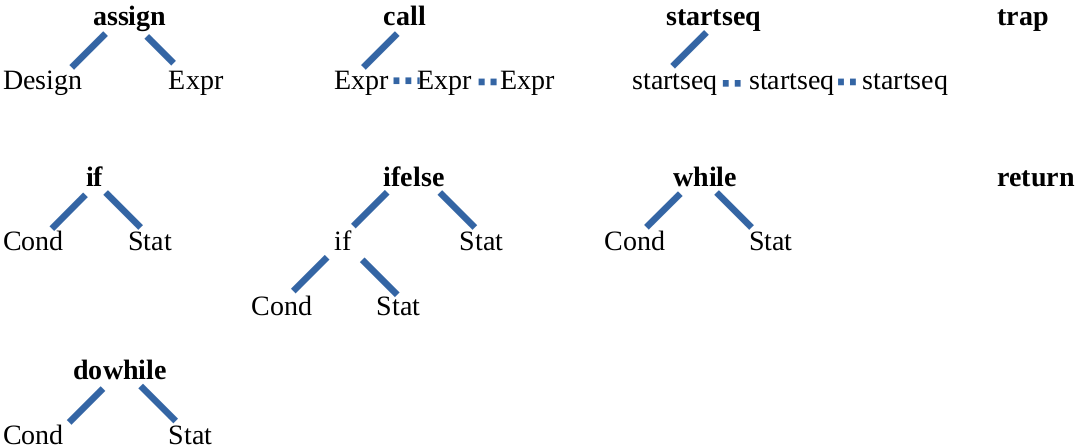
\includegraphics[width=0.9\textwidth]{./media/images/interpreter/statements.png}
  \label{fig:Statements}
\end{figure}


\subsection{Designators}
Hier kann direkt auf im Memory gespeicherte Variablen zugegriffen werden. Die von uns unterstützten Typen sind hierbei identifer, dot, und index. Diese sind für normale Variablen, Strukturen oder Arrays zuständig.

\subsection{Expressions}
Mithilfe von Expressions können verschiedene Arten von Berechnungen durchgeführt werden. Weiters werden hier auch Unterprogrammaufrufe, und Typ-Konvertierungen getätigt. Auch kann man auf im Programm definierte Konstanten zugreifen.

\subsection{Conditions}
Conditions werden von if, und Schleifen Anfragen benötigt. Mit ihnen können Vergleiche zwischen Variablen vorgenommen werden.

%\subsubsection{Just-in-time compilation}
%Um Plattformunabhängigkeit gewährleisten zu können, ist es notwendig, gewisse Teile während der Laufzeit zu kompilieren. 
%Darunter leidet aber die Ausführungsgeschwindigkeit. Deshalb wurde ein Verfahren entwickelt, welches versucht,
%diesen Nachteil zu lindern.

%Während der Anwendung des Programmes wird ein lauffähiger Maschinencode erzeugt. Es werden hierbei oft verwendete Programmteile
%während der Laufzeit kompiliert und für einen späteren Gebrauch zwischengespeichert. Hierbei ist es wichtig, dass die Compilation nicht
%zu aufwendig ist, da sonst die Geschwindigkeit des Programmes darunter leiden könnte.

\subsection{Memory System}
\label{sec:memory_system}
Während der Interpreter läuft, muss er irgendwo seine Variablen, speichern. Aus diesem Grund ist es notwendig ein geeignetes Memory System zu wählen.

%Der Call Stack wird mit einem Befehlssatz zum Befüllen, Abbauen und zum Wiedereintritt in ein anderes Unterprogramm bearbeitet.

Sobald mehrere Threads oder Prozesse ausgeführt werden sollen, muss für jeden gewünschten Prozess ein eigener Call Stack eingerichtet
werden, damit sich die Variablen und Rücksprungadressen nicht überschreiben.

\htlParagraph{Lokale Variablen:}\\
Wenn lokale Variablen verwendet werden, wird am Call Stack der nötige Variablenspeicher reserviert. Somit hat jeder Aufruf seine eigenen Variablen und den zugehörigen Speicherbereich. Dadurch sind rekursive Unterprogrammaufrufe möglich. Um vom aktuellen Aufruf auf den letzten zurückzukommen, ist es notwendig, eine Referenzadresse auf den letzten Aufruf zu speichern.

\subsection{Von uns gewähltes Memory System}
Da für kleine Programmieraufgaben, welche man zum Erlernen einer Programmiersprache, nicht viel Arbeitsspeicher benötigt wird sowie keine graphische Programmierung in C Compact vorgesehen ist, haben wir uns entschieden, 8 MB Arbeitsspeicher für den Memory zu reservieren.

In unserem Speichermodell wird zuerst eine Größe von 8MB vom Arbeitsspeicher reserviert. Dieser bietet die Grundlage. Nun werden die reservierten 8 MB halbiert. Eine Hälfte wird für Globale Variablen reserviert. Verwendete Globale Variablen werden somit einfach der reihe nach in dem für sie reservierten Speicherbereich angelegt. Die andere Hälfte wird für die Speicherung von Variablen, der Unterprogramme reserviert.

\begin{figure}[Stack Frame]
\begin{center}
\includegraphics[width=0.9\textwidth]{./media/images/interpreter/memory/stackframe.png}
\label{fig:stackframe1} 
\caption{Aufbau des von uns verwendeten Memory Systems}
\end{center}
\end{figure}
%--\includegraphics[scale=0.3]{./media/images/interpreter/memory/stackframe.png}
\htlParagraph{Speicherung der lokalen Variablen:}\\
Sobald ein Unterprogramm aufgerufen wird, wird in der oberen Hälfte der 8MB ein Speicher reserviert. Hier werden nun lokale Variablen gespeichert. Weiters werden zusätzlich noch Dynamic Link, ProcId und LineNumber gespeichert. Diese enthalten, die Rücksprungadresse, den Namen des Unterprogrammes und Zeile des Aufrufs. Der definierte FramePointer und Stackpointer zeigen hierbei den Anfang und das Ende des Speicherbereichs der lokalen Variablen an.

Wenn das Unterprogramm fertig durchlaufen ist, wird der reservierte Speicher wieder freigegeben und kann bei einem erneuten Unterprogrammaufruf genutzt werden.


%	--------------------------------------------------------
% 	Lösungsansätze
%	--------------------------------------------------------
%\section{Lösungsansätze}
%	--------------------------------------------------------
% 	Realisierte Lösungen
%	--------------------------------------------------------
%\section{Realisierte Lösungen}
%Der Interpreter wurde genauso wie die anderen Komponenten in Java implementiert.
%Am meisten wurde beim Aufbau des Interpreters auf die Schnittstelle zum GUI geachtet, da der Interpreter für eine einfachere
%Programmdarstellung optimiert werden sollte.
%
%Der Aufbau des Abstrakten Syntaxbaumes ist im Kapitel Compiler zu finden. Dort werden die einzeln verwendeten 
%Knoten näher erläutert.

%\subsection{Memory}
%Ein wesentlicher Teil des Speichermodells ist die Aufbewahrung unterschiedlichster Variablen. Hierbei wird zwischen Variablen in Unterprogrammen und globalen Variablen unterschieden. \\
%Für globale Variablen wird extra ein Platz reserviert. Lokale Variablen werden in einem gewissen Frame immer wieder auf und abgebaut. \\
%Somit bleiben globale Variablen immer enthalten, wobei Lokale Variablen nach dem Unterprogrammaufruf erstellt werden. Sobald das Unterpgramm fertig durchlaufen ist, wird der Speicherplatz der lokalen Variablen wieder freigegeben.


%\subsection{Aufbau des Memorys}
%
%Wie man in \ref{fig:stackframe1} erkennen kann, wurde dieser in zwei Hälften geteilt. Davon wird der untere Teil für globale Variablen und der obere Teil für die Unterprogramme verwendet.

%\subsection{Speicherinhalte eines Unterprogramms}
%Ein Unterprogramm muss grundsätzlich im Call Frame schon im Vorhinein einige Variablen enthalten, welche das Zurückspringen auf das letzte Unterprogramm ermöglichen. Hierfür ist der Dynamic Link zuständig. Weiters wird die LineNumber gespeichert, diese wird vom GUI benötigt, damit dieser das Programm schrittweise abarbeiten kann. Weiters ist eine ProcID vorhanden, diese ist für den Namen des Unterprogramms zuständig. Der Framepointer und der Stackpointer zeigen in unserem Fall den Start und das Ende des Variablenbereichs an.

\subsubsection{Aufruf einer neuen Methode}
Sobald der Interpreter eine neues Unterprogramm aufruft, ist es notwendig, dass der Speicherbereich für das gerade zu bearbeitende Unterprogramm reserviert wird.
\begin{enumerate}
 \item Zuerst werden 4 Byte für die Zeilennummer reserviert. Die Zeilennummer wird von der Entwicklungsumgebung zum zurückspringen benötigt.
 \item Nun wird der Methodenname im Speicher vermerkt, dieser hat eine Größe von 4 Byte und wird bei der Anzeige in der Benutzeroberfläche verwendet.
 \item Um ein Unterprogramm ordnungsgemäß schließen zu können, ist eine Referenz zum vorher verwendeten Speicherbereich notwendig. Diese Referenz enthält die Daten des zuletzt verwendeten Framepointers und besitzt eine Größe von 4 Byte.
 \item Sobald diese Daten gespeichert wurden, kann nun die Adresse des Framepointers auf die des Stackpointers gesetzt werden.
 \item Um den Speicherbereich der lokalen Variablen zu reservieren, muss der Stackpointer um die vom Compiler vorgegebene Größe erhöht werden.
\end{enumerate}
 
\subsubsection{Schließen einer Methode}
\begin{enumerate}
 \item Zuerst wird der reservierte Variablenspeicher wieder freigegeben. Dies geschieht in dem man den Wert des Stackpointers mit dem Wert des Framepointers überschreibt.
 \item Um nun mit dem aktuell arbeitenden Unterprogramm weiterarbeiten zu können, muss der reservierte Variablenbereich wiederhergestellt werden. Dies kann gemacht werden, indem man die im Dynamic Link gespeicherte Adresse ausließt und diese im Framepointer speichert. Somit, müssen nun vom Stackpointer 4 Bytes abgezogen werden und der darin enthaltene Wert muss auf den Framepointer übertragen werden.
 \item Nun muss nur mehr der Stackpointer richtig gestellt werden. Dies geschieht indem man den Stackpointer um den vorherigen Methodennamen und die vorher verwendete Zeilennummer verringert. Somit muss der Stackpointer um 8 Byte verringert werden.
\end{enumerate}

\subsubsection{Speicherverwaltung}
Da bei der Speicherverwaltung viele Fehler auftreten könnten, ist es wichtig, dass diese mit verschiedensten Exceptions abgefangen werden.

Alle vom Interpreter benötigten Funktionen sind in der statischen Klasse Memory zu finden. 

Vom dem von uns gewählten Memory System werden verschiedenste Datentypen unterstützt.
\begin{itemize}
 \item int - 4 Byte
 \item float - 4 Byte
 \item char - 2 Byte 
 \item boolean - 1Byte
 \item string - 4 Byte - beinhaltet jedoch nur die Adresse des Strings. Durch diese Implementationsart, können Strings in C Compact nicht wie in C verwendet werden, sondern sie sind sehr Java ähnlich.
\end{itemize}
Damit nun der Interpreter den Speicher verwenden kann, sind in der Memory Klasse verschiedenste Methoden vorhanden, welche zum Laden und Speichern von Variablen dienen.

Sobald eine Variable gespeichert wurde, wird zusätzlich noch gespeichert, ob die verwendete Variable bereits initialisiert wurde.
\begin{lstlisting}[language=JAVA]
	public static void storeInt(int address, int value) {
		changedVariables.add(address);
		getMemoryInformation(address).isInitialized = true;
		memory.putInt(address, value);
	}
\end{lstlisting}

\begin{lstlisting}[language=JAVA]
	public static int loadInt(int address) {
		readVariables.add(address);
		return memory.getInt(address);
	}
\end{lstlisting}

%\subsection{Interpreter}
%Weil wir eine einfache Darstellung der aktuellen Variablen bezweckten und den Ablauf des Programmes nicht verändern wollten, kam für 
%uns nur der Abstrakte Syntaxbaum-Interpreter in Frage.
%
%Es wurden einige Vorgaben gemacht, um ein Zusammenarbeiten zwischen Compiler und Interpreter möglich zu machen. Somit wurde eine gewisse
%Baumstruktur vorgegeben. In dieser konnten die Knoten nur in einer bestimmten Reihenfolge auftreten.
%
%Somit wurde der Interpreter so gestaltet, dass dieser Abstrakte Syntax Baum systematisch abgearbeitet wird. Dies wurde durch Unterteilen in verschiedene Klassen erledigt, welche systematisch abgearbeitet werden.
%
%\subsection{Statements}
%Statements haben im Vergleich zu Expressions nicht immer einen Wert, jedoch können durch Expressions Variablen zugewiesen, Schleifen gestartet oder andere Methoden ausgeführt werden. Dies hier ist die erste Methode, welche nach der Startsequenz ausgeführt wird. Somit gelangt man von dieser Methode zu fast allen anderen Methoden.
%
%\subsubsection{assign}
%Bei einem Assign wird eine bestimmte Variable in den Memory geschrieben. Bevor dies jedoch geschehen kann, ist es notwendig,
%den Datentyp herauszufinden. Dafür wird der Typ des rechten Knotens geprüft. Weiters wird am rechten Knoten eine Expression erwartet, das bedeutet, dass hier auch zum Beispiel Berechnungen vorgenommen werden können.
%
%\includegraphics[width=0.4\textwidth]{./media/images/interpreter/syntaxbaum/statements/assign.png}
%
%\subsubsection{Startsequenz}
%Mithilfe der Startsequenz wird das derzeitige Unterprogramm abgearbeitet und zum schrittweisen Durchgehen des Programmes benötigt. Sobald der Interpreter abgebrochen wurde, kann es hier wieder gestartet werden. Dies geschieht, indem die Startsequenz wieder die notwendige letzte bekannte Node bekommt.
%
%\includegraphics[width=0.6\textwidth]{./media/images/interpreter/syntaxbaum/statements/startsequenz.png}
%
%\subsubsection{trap}
%Falls ein Unterprogramm keinen Rückgabewert besitzt, muss dieses trotzdem beendet werden, ohne verschiedene Errors zu erzeugen. Aus diesem Grund wurde eine Trap eingeführt, diese beendet das Unterprogramm, ohne einen Rückgabewert zu speichern.
%
%\subsubsection{if}
%Durch diesen Node ist es möglich, bestimmte Verzweigungen im Programm zu schaffen. Auf der linken Seite des Knotens stehen die Bedingungen, auf der rechten Seite das auszuführende Programm, wenn die Bedingung true ergibt.
%
%\includegraphics[width=0.4\textwidth]{./media/images/interpreter/syntaxbaum/statements/if.png}
%
%\subsubsection{Ifelse}
%Das Ifelse ist grundsätzlich genauso aufgebaut wie das If. Der wesentliche Unterschied besteht darin, dass, sobald die Condition
%false ergibt, die andere if-Funktion abgearbeitet wird.
%
%\includegraphics[width=0.4\textwidth]{./media/images/interpreter/syntaxbaum/statements/ifelse.png}
%
%\subsubsection{while}
%Sie funktioniert ähnlich wie ein If, das Statement jedoch wird so oft wiederholt, bis die Condition false ergibt.
%
%\includegraphics[width=0.4\textwidth]{./media/images/interpreter/syntaxbaum/statements/while.png}
%
%\subsection{call}
%\includegraphics[width=0.6\textwidth]{./media/images/interpreter/syntaxbaum/statements/call.png}
%
%Ein Call-Knoten hat mehrere Funktionen, die Richtige wird anhand des Namens herausgefunden. Dies sind schon vordefinierte
%Funktionsnamen, welche in einem Programm nicht erneut verwendet werden können.
%
%Hier eine Auflistung dieser Funktionen:
%
%\subsubsection{print}
%Hiermit wird ein Char-Zeichen dem StdInOut Interface übergeben. Somit kann dieses danach vom GUI ausgeben werden.
%
%\subsubsection{read}
%Wenn Read aufgerufen wird, werden vom Interface StdInOut Char-Variablen eingelesen und diese als Return-Wert gesetzt, der somit zur Weiterverarbeitung verwendet werden.
%
%\subsubsection{length}
%Hier kann man die Länge eines Strings bestimmen lassen, der wiederum als Return-Wert gesetzt.
%
%\subsubsection{time}
%``time'' dient zum Bestimmen der Zeit, welche wiederum als Return-Wert zurückgegeben wird. Wird für den implementierten Zufallsgenerator bei der Initialisierung benötigt.
%
%\subsubsection{Normaler Aufruf}
%%TODO Neu programmiert
%Sobald ein Aufruf erfolgt, werden alle Variablen, welche übergeben werden sollen, in einem Objekt zwischengespeichert. Nun kann ein
%neues Memoryframe geöffnet werden. Die Variablen, welche in einem Objekt zwischengespeichert wurden, können nun in das neue
%Memoryframe übertragen werden.
%
%Nun wird eine Startsequenz ausgeführt, damit der Unterprogrammaufruf abgearbeitet werden kann.
%
%\subsection{Designators}
%Auf Designators werden bestimmte Werte gespeichert. Diese können zum Beispiel normale Variablen, Arrays oder Strukturen sein. Hier ist die richtige Zuweisung der Adresse wichtig.
%
%Designators werden in drei Grundtypen unterschieden:
%\subsubsection{Identifer}
%Ein Identifer ist eine normal,e einfache Variable. Wenn ein Identifer aufgerufen wird, werden verschiedene Faktoren geprüft.
%\begin{itemize}
% \item Falls diser global ist, wird der Globalpointer mit der Objektadresse addiert.
% \begin{lstlisting}[language=JAVA]
% adr = Memory.getGlobalPointer() + obj.adr;	
%  \end{lstlisting}
%  Trifft voriges nicht zu, wird anstelle des Globalpointers der Framepointer des aktuellen Aufrufes zur Objektadresse addiert.
%   \begin{lstlisting}[language=JAVA]
% adr = Memory.getFramePointer() + obj.adr;
%  \end{lstlisting}
% \item Wenn der Identifer eine Referenz auf eine Adresse ist, wird hier die gespeicherte Adresse geladen.
%\end{itemize}
%
%
%
%\subsubsection{Dot}
%\includegraphics[width=0.4\textwidth]{./media/images/interpreter/syntaxbaum/designators/dot.png}
%
%Dieser Knoten wird für Strukturen angewandt. Um die richtige Adresse für eine Variable in der Struktur zu bekommen, muss die Adresse des linken
%Knotens mit der rechten Seite des Knotens addiert werden.
%
%\begin{lstlisting}[language=JAVA]
%return Adr(p.left) + p.right.val
%\end{lstlisting}
%
%\subsubsection{Index}
%\includegraphics[width=0.4\textwidth]{./media/images/interpreter/syntaxbaum/designators/index.png}
%Der Index wird vom Array verwendet. Um den Index des gewünschten Arrays auszurechnen, ist es notwendig, die Expression des rechten Knotens aufzulösen.
%Nun kann die Adresse berechnet werden. Diese setzt sich aus dem Produkt der Adresse des rechten Knotens und der  Speicherbedarf eines einzelnen Indexelementes zusammen.
%
%\begin{lstlisting}[language=JAVA]
%return Adr(p.left) + p.left.type.elemType.size * index;
%\end{lstlisting}
%
%\subsection{Expressions}
%Expressions werden grundsätzlich für Berechnungen und Typkonvertierungen verwendet. Aus diesem Grund ist es wichtig, dass jeder Datentyp seine eigene Expressions-Methode besitzt. Weiters können hier Konstanten abgefragt werden.
%
%\subsection{Conditions}
%Conditions werden für Vergleiche und für die Verwendung von if-Bedingungen sowie Schleifen benötigt. Weiters dienen sie auch zum Verknüpfen mehrerer Conditions.
%
%Hier wird unterschieden zwischen:
%\begin{itemize}
%\item EQL: Überprüft, ob das Element auf der rechten Seite gleich dem der linken Seite ist.
%\item NEQ: Die Variable des linken Knotens darf der des rechten Knotens nicht gleichen.
%\item LSS: Das Element der linken Seite muss kleiner sein als das der rechten.
%\item LEQ: Die Variable des linken Knotens darf gleich und kleiner sein als die Variable des rechten.
%\item GTR: Gibt true zurück, wenn die Variable des linken Knotens größer ist als die des rechten Knotens.
%\item GEQ: Überprüft, ob das Element auf der rechten Seite gleich oder größer dem der linken Seite ist.
%\item OR: Überprüft zwei Conditions mithilfe eines Operators.
%\item AND: Zwei Conditions werden hiermit mit einem verknüpft.
%\item NOT: Der gegebene linke Knoten ist eine Condition. Diese wird negiert zurückgegeben.
%\item CALL: Ruft ein Unterprogramm auf, welches den Rückgabewert, den Datentyp Boolean hat. Dies kann somit für eine Abfrage weiterverwendet werden.
%\end{itemize}

\subsection{Aufbau des Interpreters}
Der Interpreter wurde so gestaltet, dass der Abstrakte Syntax Baum systematisch abgearbeitet wird. Damit dies möglich ist wurde er in mehrere Methoden gespaltet. Jede Methode ist für die Verarbeitung eines kleinen Teils des AST zuständig. Dies ist notwendig, da sich oftmals Methoden selbst wieder aufrufen.

Zum Starten des Interpreters wird zuerst Startseq() gestartet und der dazugehörige Knoten übergeben. Die Methode sorgt mit einer for Schleife dafür, dass alle verfügbaren Knoten verarbeitet werden. Nun wird ein Statement aufgerufen. 
\begin{itemize}
\item Falls der Knoten nun ein Assign, also eine Zuweisung ist, muss zuerst der Datentyp überprüft werden. Nun wird die rechte Seite des Knotens mit der zugehörigen Expression-Methode weiterverarbeitet und dann in der Adresse des linken Knotens gespeichert, dieser wird mithilfe eines Designators-Knoten definiert.
\item Hier kann nun auch ein Knoten auftreten, bei welchem eine if, ifelse, while oder do-while Abfrage stattfindet. Hierfür werden die nötigen Knoten einfach mit den javainternen Funktionen überprüft. Somit wird zum Beispiel, beim Aufruf eines if-Knotens, der Linke Knoten mithilfe einer Condition mit der Java If-Abfrage geprüft, wenn dieser true ergibt, wird mit dem rechten Knoten weitergearbeitet.
\item Falls der aktuell abgerufene Knoten ein Return ist, so wird im Memory der notwendige Return-Wert gespeichert. Hierbei ist zu beachten, dass zwischen den Datentypen unterschieden werden muss.
\item Wenn dieser Knoten auftritt, ist im Benutzerprogramm kein Return vorhanden und es wird eine Exception geworfen.
\item Der Knoten kann auch den Wert \textit{break} oder \textit{continue} haben. Diese lösen eine jeweils zugehörige Exception aus, welche von den gerade verwendeten Schleifen abgefangen und weiterverarbeitet werden.
%TODO For
%TODO Switch CASE
\end{itemize}

\subsubsection{Designator}
Designators verweisen auf bestimmte Adressen im Memory. Dort werden Variablen des Benutzerprogramms gespeichert. Ein Designator kann zum Beispiel eine normale Variable, ein Array oder eine Struktur sein. Grundsätzlich werden Designators in drei Grundtypen unterschieden.

\htlParagraph{Identifer}\\
Ein Identifer ist eine normale, einfache Variable. Falls der gerade bearbeitende Knoten ein Identifer ist, werden verschiedene Faktoren geprüft.
\begin{itemize}
 \item Mithilfe einer im Knoten gespeicherten Variable Namens p.obj.level, kann herausgefunden werdenm ob es sich hierbei um eine Globale Variable handelt.Ist dies der Fall wird der Globalpointer, welcher in der Klasse Memory mit der Objektadresse addiert.
 \begin{lstlisting}[language=JAVA]
 adr = Memory.getGlobalPointer() + obj.adr;	
  \end{lstlisting}
Ist die Adresse jedoch nicht Global, wird anstelle des Globalpointers der Framepointer des aktuellen Unterprogramms zur Objektadresse addiert.
   \begin{lstlisting}[language=JAVA]
 adr = Memory.getFramePointer() + obj.adr;
  \end{lstlisting}
 \item Falls es sich bei dem Identifer um eine Referenz handelt, was in der p.obj.isRef definiert ist. Wird die darin gespeicherte Adresse geladen und als zurückgegeben.
\end{itemize}

\htlParagraph{Dot}\\
%\includegraphics[width=0.4\textwidth{./media/images/interpreter/syntaxbaum/designators/dot.png}
Dieser Knoten wird für Strukturen verwendet. Dadurch, dass der Linke Knoten ein Designator ist, sind können hier Strukturen in Strukturen gespeichert werden. Der Rechte Knoten, ist hierbei eine Konstante, sie beinhaltet die Datengröße der Variable. Um die richtige Adresse für eine Variable in der Struktur zu bekommen, muss somit die Adresse des linken
Knotens mit der rechten Seite des Knotens addiert werden.

\begin{lstlisting}[language=JAVA]
return Adr(p.left) + p.right.val
\end{lstlisting}

\htlParagraph{Index}\\
%\includegraphics[width=0.4\textwidth{./media/images/interpreter/syntaxbaum/designators/index.png}
Der Index wird vom Array verwendet. Um den Index des gewünschten Arrays auszurechnen, ist es notwendig, die Expression des rechten Knotens aufzulösen.
Nun kann die Adresse berechnet werden und der Variablenwert somit ausgelesen werden. Diese setzt sich aus dem Produkt der Adresse des rechten Knotens und der Speicherbedarf eines einzelnen Indexelementes zusammen.

\begin{lstlisting}[language=JAVA]
return Adr(p.left) + p.left.type.elemType.size * index;
\end{lstlisting}

\subsection{Aufbau einer Condition}
Beim Aufruf eine Condition, muss zwischen den Unterschiedlichen Datentypen unterschieden werden. Der Datentyp kann beim Linken Knoten abgefragt werden.

Mithilfe eines Switch-Case kann nun zwischen den verschiedenen Vergleichsoperatoren unterschieden werden. Nun wird die Linke und die Rechte Expression aufgelöst. Beide Expressionen werden nun mit den Javainternen Funktionen verglichen. 
\begin{lstlisting}[language=JAVA]
case Node.EQL:
	return IntExpr(p.left) == IntExpr(p.right);
\end{lstlisting}

Wenn es sich bei dem Knoten um ein or oder and handelt, werden der Linke beziehungsweise der Rechte Knoten wiederum als Condition betrachtet, und beide mit einem if verglichen. Falls der Knoten ein Not ist, wird nochmals eine Condition ausgeführt, welche danach negiert wird.
\begin{lstlisting}[language=JAVA]
case Node.NOT:
	return !Condition(p.left); // NOT
\end{lstlisting}

Hier kann auch ein Call aufgerufen werden, welcher als Rückgabe-Wert boolean besitzt.

\subsubsection{Abarbeitung einer Expression}
Jeder Datentyp hat seine eigene Expression. Grundsätzlich werden diese für Rechenoperationen und Typ-Konvertierungen benötigt. Für Berechnungen werden jeweils der linke Knoten und der fechte Knoten wieder an die eigene Klasse weitergegeben. Dies geschieht um komplexere Rechenbeispiele lösen zu können. 
\begin{lstlisting}[language=JAVA]
case Node.PLUS:
if(p.right == null)
	return IntExpr(p.left);
else
	return SaveIntOperator.add(IntExpr(p.left),IntExpr(p.right));
\end{lstlisting}

Da C-Compact ein Feature implementiert hat, welches Adressen mitloggt, die bereits beschrieben wurden, wird bei dem Aufruf einer nicht initialisierten Variable eine Exception geworfen. Um Überlaufen von Integer Werten zu vermeiden, werden Berechnungen mithilfe SaveIntOperator und SaveFloatOperator ausgeführt.

\begin{lstlisting}[language=JAVA]
	public static final int add(int left, int right) throws ArithmeticException {
		if (right > 0 ? left > Integer.MAX_VALUE - right
           : left < Integer.MIN_VALUE - right) {
			throw new ArithmeticException("Integer overflow");
		}
		return left + right;
	}
\end{lstlisting}

In einer Expression können jedoch auch Typ-Konvertierungen und Unterprogrammaufrufe stattfinden.

\htlParagraph{Typkonvertierungen}\\
Für jeden Datentyp wurde eine notwendige Expressions-Methode implementiert. Somit muss zu jedem Datentyp die richtigen Funktionen zum Konvertieren von anderen Typen in den eigenen vorhanden sein. So besitzt zum Beispiel eine Int-Expression Funktionen, mit denen es erlaubt ist float, char und boolean zu int zu konvertieren.
Im Interpreter wurde dies mithilfe der Java-internen Funktionen eingebunden. 

\begin{lstlisting}[language=JAVA]
case Node.F2I:
		return (int) FloatExpr(p.left);
\end{lstlisting}


\htlParagraph{Laden von Konstanten}\\
Da in C Compact auch Konstanten definiert werden können, müssen diese auch irgendwo ausgelesen werden. Den Wert, den die Konstante hat, wird direkt im Knoten definiert. Aus diesem Grund, muss er nur mehr von der richtigen Expression-Methode im Interpreter ausgelesen werden.

\begin{lstlisting}[language=JAVA]
case Node.INTCON:
		return p.val;
\end{lstlisting}

%TODO
\subsubsection{Das Aufrufen eines Calls}
Ein Call besitzt mehrere Basisfunktionen, diese können nicht erneut vom Benutzer als Funktion definiert werden und besitzen einen vorgegebenen Ablauf.

\htlParagraph{print}\\
Beim Aufruf dieser Basismethode, wird ein Char-Zeichen ausgegeben.
\begin{lstlisting}[language=JAVA]
inout.out(CharExpr(p.left));
\end{lstlisting}

\htlParagraph{read}\\
Wenn read aufgerufen wird, werden vom Interface StdInOut Char-Variablen eingelesen und diese als Return-Wert gesetzt, der somit zur Weiterverarbeitung verwendet werden.
\begin{lstlisting}[language=JAVA]
Memory.setCharReturnValue(inout.in());
\end{lstlisting}

\htlParagraph{length}\\
Mit dieser Methode kann die Länge eines String bestimmt werden, der wiederum als Return-Wert gesetzt. Hier wird eine Exeption geworfen, falls zu dieser Klasse Kein String übergeben wird.
\begin{lstlisting}[language=JAVA]
case Struct.STRING:	Memory.setIntReturnValue(Strings.get(StringExpr(p.left)).length());
\end{lstlisting}

\htlParagraph{time}\\
``time'' dient zum Bestimmen der Zeit, welche wiederum als Return-Wert zurückgegeben wird. Wird für den implementierten Zufallsgenerator, bei der Initialisierung benötigt.
\begin{lstlisting}[language=JAVA]
Memory.setIntReturnValue((int)(date.getTime()/1000));
\end{lstlisting}

\htlParagraph{printf}\\
Auf der Linken Seite des Knotens, wird der String ausgewertet. Nun werden an den Stellen wo ein \% steht, die Variablen welche angegeben wurden eingefügt. Hierbei wird mit einem switch-case unterschieden um welche Art es sich hierbei handelt.
\begin{itemize}
\item d, steht für eine int Variable. Wenn dies Aufgerufen wird, werden die Variable die hierbei angegeben wurde, in eine Int Variable konvertiert und danach als String ausgegeben
\item x, steht für eine Hex Zahl. Die dafür angegebene Variable wird nun in eine Int Zahl konvertiert und als Hex-Zahl ausgegeben.
\item f, steht für eine Float Variable, die angegebene Variable wird somit in eine Float Zahl konvertiert und als String ausgegeben.
\item c, steht für einen Charakter, die Variable wird konvertiert und ausgegeben. 
\end{itemize}
Schlussendlich kann der zusammengesetzte String vom dem InOut Interface an die Benutzeroberfläche übergeben werden.

\htlParagraph{Normaler Aufruf}\\
Wird ein im Benutzerprogramm erstelltes Unterprogramm aufgerufen wird ein normaler Call ausgeführt. Als erstes wird der aktuelle Framepointer zwischengespeichert. Nun wird im Memory ein neues Frame angelegt[\ref{}], dadurch wird der Framepointer und der Stackpointer auf das neue Frame gesetzt.

Nun können die Parameter ins neue Frame geschrieben werden. Jetzt wird ein Node erstellt, welcher die Expressions des Calls beinhaltet. Diese werden aufgelöst und in das neue Frame übertragen. 
\begin{lstlisting}[language=JAVA]
Memory.storeBool(newFramePointer + form.adr, BoolExpr(ref));
\end{lstlisting}
Falls eine Referenz übergeben wird, wird die Adresse übertragen. Nun kann eine neue Startsequenz ausgeführt werden.

Sobald das Unterprogramm fertig durchlaufen ist, wird der aktuelle Frame wieder geschlossen und somit der lokale Variablenspeicher wieder freigegeben.

\htlParagraph{Funktion eines Returns}\\
Unterprogramme in C Compact können genauso wie in C auch Return-Werte besitzen. Sobald ein Unterprogramm, in einer Expression gestartet wurde, wird sobald ein Return-Knoten erreicht wurde, eine Return-Exception ausgelöst und der Rückgabewert im Memory vermerkt. Dieser kann nach der Schließung des Frames wieder entnommen und weiterverarbeitet werden.
\begin{lstlisting}[language=JAVA]
Call(p);
return Memory.getIntReturnValue();	
\end{lstlisting}

Der Trap Knoten wird dient zur Identifizierung von Unterprogrammen, welche einen Return Wert besitzen müssten, dieser jedoch nicht gesetzt wurde. Sobald dieser ausgelöst wird, wird eine RunTimeException geworfen.
\begin{lstlisting}[language=JAVA]
case Node.TRAP:
throw new RunTimeException("Return Statement missing", p, currentLine); 
\end{lstlisting}

\fi

% Benutzeroberfläche, Debugger
\iffabian
	%!TEX root = "../../DA_GUI.tex"

%	--------------------------------------------------------
% 	Aufbau der Benutzeroberfläche
%	--------------------------------------------------------

\chapter{Elemente der Benutzeroberfläche}
In diesem Kapitel wird der grundlegende Aufbau aller Fenster und Benutzeroberflächen von C Compact beschrieben - sowohl die konzeptuelle Konstruktion als auch die Implementierung.
\section{Das Konzept}
Das Aussehen und die Bedienung von C Compact folgt durchgehend der grundlegenden Idee, eine einfach und intuitiv zu bedienende Entwicklungsumgebung zu schaffen. Das bedeutet, Features möglichst Zielgruppenorientiert zu integrieren und überflüssige Funktionen zu vermeiden. Bei der Entwicklung wurde besonders auf Vollständigkeit und logische Bedienvorgänge geachtet, um eine konsistente und verständliche Bedienung zu ermöglichen.
%TODO TODO read last sentence
%Durch besondere Rücksicht auf Vollständigkeit und logische Bedienvorgänge haben wir ein durchgängig logisches Bedienerlebnis angestrebt.
%Konkret haben wir uns dabei an folgende Regeln gehalten:

C Compact wurde deshalb nach folgenden Richtlinien entwickelt:
\begin{itemize}
\item Das Aussehen und die Positionierung von Elementen in der Benutzeroberfläche soll logisch begründbar sein
\item Funktionen, die im FSST-Unterricht der ersten und zweiten Klassen wahrscheinlich nicht benötigt werden, werden vermieden oder sind standardmäßig deaktiviert; Bedienelemente werden also auf das wesentlichste reduziert
\item Wir sind der Meinung, dass eine intuitiv zu bedienende Oberfläche nicht durch Animationen und große Symbole erzielt werden kann, sondern durch einfache, bereits bekannte Konzepte. So sind in C Compact bekannte Elemente wie beispielsweise eine Menüleiste mit gewohnten Datei- und Dokumentoperationen zu finden (Siehe Kapitel \ref{sec:gui-main-menu}).
\end{itemize}

\subsection{Daraus resultierende Einschränkungen}
Durch diese Reduktion der gesamten Oberfläche ist C Compact auf einen bestimmten Zweck, die Ausbildung, beschränkt. Das sehen wir allerdings nicht als Nachteil, sondern als besondere Stärke. Mit C Compact wollen wir eine Entwicklungsumgebung schaffen, die Anfänger nicht überfordert und ihnen hilft, sich auf das wesentliche zu konzentrieren.
Das Konzept einer anfängerfreundlichen Entwicklungsumgebung ist mit dem Aufbau einer Umgebung für die professionelle Entwicklung nicht vereinbar. C Compact soll aber auf späteres Arbeiten mit komplexeren Programmen vorbereiten. Schüler, die ihre erste Programmiersprache mit C Compact erlernen, kennen bereits den Umgang mit einem Debugger und haben ein tieferes Verständnis für den Ablauf von Programmen.

%TODO add window desc. for launcher, quest seleter, package selecter
\section{Fenster Der Benutzeroberfläche}
Neben dem Hauptfenster, das den Kern der Benutzeroberfläche darstellt, gibt es eine Reihe von kleineren Aktionsfenster, Dialogen und Einstellungsfenstern, die zum reibungslosen Ablauf bei der Bedienung von C Comapct beitragen. Das Hauptfenster selbst wird in Kapitel \ref{sec:gui-main} beschrieben.

\subsection{Launcher}
\label{sec:win-launcher}
...

\subsection{Einstellung der Sprache}
\label{sec:win-lang}
Wenn C Compact zum ersten Mal gestartet wird, wird zuallererst dieses Fenster angezeigt. Der Benutzer wird gebeten, eine Sprache zu wählen. Später kann die Sprache über das Menü \glqq{}Datei\grqq{} im Hauptfenster (Siehe Kapitel \ref{sec:gui-main-menu-file}) geändert werden. Die Änderungen werden erst wirksam, wenn der Benutzer die neue Sprache mit \glqq{}OK\grqq{} bestätigt (siehe auch Kapitel \ref{sec:lang}). Dann wird C Compact neu gestartet.

\begin{figure}[htp]
\centering
\includegraphics[width=0.3\textwidth]{./media/images/gui/elements/Bildschirmfoto-Sprache.png}
\caption{Auswahl der Sprache}
\label{fig:win-lang}
\end{figure}

Dieses Fenster ist in der Klasse \textbf{GUILanguage} im Package \textbf{at.jku.ssw.cmm.gui.properties} implementiert. 

\subsection{Allgemeine Einstellungen}
\label{sec:win-set}
Dieses Fenster enthält allgemeine Optionen zum Haupfenster der Benutzeroberfläche (siehe Kapitel \ref{sec:guimainsettings}). Es kann im Menü des Hauptfensters unter \glqq{}Datei\grqq{} - \glqq{}Einstellungen\grqq{} aufgerufen werden (Siehe Kapitel \ref{sec:gui-main-menu-file}). Änderungen an den Einstellungen werden sofort wirksam (ausgenommen sind Änderungen an der Schriftgröße von Dokumenten). Da C Compact beim Ändern dieser Einstellungen nicht neu gestartet werden muss, sind diese Optionen und die Spracheinstellungen in zwei unterschiedliche Fenster aufgeteilt.
%TODO ref load html->font size

\begin{figure}[htp]
\centering
\includegraphics[width=0.4\textwidth]{./media/images/gui/elements/Bildschirmfoto-Einstellungen.png}
\caption{Einstellungsfenster}
\label{fig:win-set}
\end{figure}

Im Einstellungsfenster können folgende Optionen verändert werden:
\begin{enumerate}
\item \textbf{Ansicht:} Ändert den Aufbau des Hauptfensters. Elemente werden je nach gewähltem Layout unterschiedlich angeordnet. Siehe Kapitel \ref{sec:gui-main-left-ord}.
\item \textbf{Schriftgröße des Sourcecode:} Ändert die Schriftgröße des Textfeldes für den Sourcecode im Hauptfenster. Siehe Kapitel \ref{sec:gui-main-left-code}.
\item \textbf{Schriftgröße der Textfelder:} Ändert die Schriftgröße der Textfelder für Ein- und Ausgabedaten im Hauptfenster. Siehe Kapitel \ref{sec:gui-main-left-io}.
\item \textbf{Schriftgröße von Dokumenten:} Dokumente, wie etwa Beschreibungstexte von Fehlern (siehe Kapitel \ref{sec:deb-error}), können mit unterschiedlichen Textgrößen angezeigt werden. Da die Schriftgröße beim Initialisieren der Textfelder festgelegt wird, betrifft die Einstellung immer nur die Dokumente, die in Zukunft geöffnet werden.
%TODO ref Fehlerdokumente
\item \textbf{Rückgabewerte anzeigen:} Der Debugger kann den Rückgabewert einer Funktion in einem Popup (siehe auch Kapitel \ref{sec:deb-popup}) darstellen. Da dieses Feature nicht immer hilfreich ist, ist es standardmäßig deaktiviert.
\end{enumerate}

Alle Klassen des Einstellungsfensters befinden sich im Package \textbf{at.jku.ssw.cmm.gui.properties}. Das Fenster selbst wird in der Klasse \textbf{GUIProperties} initialisiert, Listener für alle Schieberregler befinden sich in der Klasse \textbf{PropertiesSliderListener}. Die Combobox für das Layout der Benutzeroberfläche (Option 1) wird mit der Klasse \textbf{PropertiesComboListener} überwacht, die Checkbox für das Anzeigen von Rückgabewerten im Debugger ist mit dem ActionListener \textbf{PropertiesActionListener} verknüpft.

Beim Ändern der Schriftgröße werden zuerst die Einstellungen von C Compact verändert, dann werden die Schriftgrößen in den entsprechenden Elementen aktualisiert.
\begin{lstlisting}[language=JAVA]
@Override
public void stateChanged(ChangeEvent e) {
	JSlider slider = (JSlider)e.getSource();
	
	// Einstellungen aktualisieren
	main.getSettings().setCodeSize(GUIProperties.sliderPosToFont(slider.getValue()));
	
	// Schriftgrößen aktualisieren
	master.updateTextSize();
}
\end{lstlisting}

Tatsächlich wird beim aktualisieren der Schriftgrößen in Textfeldern einfach ein neuer Font mit der entsprechenden Größe aus dem bereits verwendeten Font abgeleitet und angewandt.
\begin{lstlisting}[language=JAVA]
// Schriftart (font) ändern
this.jSourcePane.setFont(
	// Aktuellen Font ableiten
	this.jSourcePane.getFont().deriveFont(
		//Schriftgröße laut Einstellungen
		(float)this.main.getSettings().getCodeSize()
	)
);
\end{lstlisting}

\subsection{Über C Compact}
\label{sec:win-credits}
% !!! TODO mention SSW in credits !!!
Dieses Fenster enthält den Lizenztext von C Compact sowie die Namen der beteiligten Personen. Auch dieses Fenster kann im Menü der Entwicklungsumgebung aufgerufen werden (Menü siehe Kapitel \ref{sec:gui-main-menu-file}). Alle Bestandteile dieses Elementes befinden sich im Package \textbf{at.jku.ssw.cmm.gui.credits}:
\begin{itemize}
\item \textbf{Credits.java:} Initialisiert das Fenster und regelt sein Verhalten.
\item \textbf{credits.html:} Enthält den Lizenztext.
\item \textbf{credits.css:} Enthält Formatierungsinformationen zum Lizenztext.
\end{itemize}
%TODO ref Dokumente laden

Die Resourcen sind im Package eingebunden und deshalb auch Teil der generierten JAR-Datei. Dadurch kann der Lizenztext nicht einfach verändert werden.

\begin{figure}[htp]
\centering
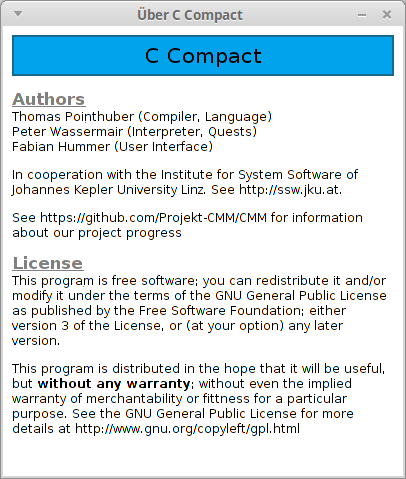
\includegraphics[width=0.4\textwidth]{./media/images/gui/elements/Bildschirmfoto-About.png}
\caption{Fenster mit Lizenztext}
\label{fig:win-about}
\end{figure}

\subsection{Questpacket auswählen}
...

\subsection{Quest auswählen}
...

\subsection{Profil erstellen}
... name eingeben ...

\subsection{Dialoge}
\label{sec:win-dialog}
In C Compact werden viele verschiedene Dialogfenster verwendet. Der Begriff Dialogfenster\footnote{http://de.wikipedia.org/wiki/Dialog\_(Benutzeroberfläche)} umfasst eine Reihe von unterschiedlichen Anwendungen, bei denen ein Fenster verwendet wird, um Informationen oder Befehle vom Benutzer einzuholen. Dialoge werden in C Compact beispielsweise verwendet, um zu fragen, ob eine Datei gespeichert werden soll (Abbildung \ref{fig:win-dialog}), oder um den Benutzer auf ein Problem aufmerksam zu machen. Swing enthält bereits einige Funktionen zum Erstellen von Dialogen\footnote{http://docs.oracle.com/javase/tutorial/uiswing/components/dialog.html}, anhand dieses Tutorials können einfache Dialoge sehr schnell erstellt werden.

\begin{figure}[htp]
\centering
\includegraphics[width=0.4\textwidth]{./media/images/gui/elements/Bildschirmfoto-Dialog.png}
\caption{Ein einfacher Dialog}
\label{fig:win-dialog}
\end{figure}

\subsection{Dateimanager}
...

%TODO add information about info saved in profiles
\section{Einstellungen}
\label{sec:guimainsettings}
Für den Betrieb einer Benutzeroberfläche ist es unerlässlich, diese anpassbar zu machen und Anpassungen des Benutzers zu speichern. Im Package \textbf{at.jku.ssw.cmm.gui.properites} befindet sich die Klasse \textbf{GUImainSettings}, die alle globalen Einstellungen verwaltet und speichert. Diese Einstellungen umfassen:
\begin{itemize}
\item Die zuletzt geöffneten Dateien
\item Die gerade geöffnete Datei
\item Die zuletzt geöffneten Benutzerprofile
\item Das aktuell aktive Benutzerprofil
\item Die vom Benutzer gewählte Sprache (siehe Kapitel \ref{sec:lang})
\item Einstellungen, die der Benutzer direkt verändern kann (Siehe Kapitel \ref{sec:win-set})
\begin{itemize}
\item Schriftgrößen
\item Layout der Benutzeroberfläche
\end{itemize}
\end{itemize}

Bevor das Hauptfenster der Entwicklungsumgebung gestartet werden kann, muss ein Objekt der Klasse \textbf{GUImainSettings} erstellt werden (Siehe dazu Kapitel \ref{sec:gui-main-impl}). Dabei werden die zuletzt gespeicherten Einstellungen geladen.

Die Einstellungen werden in der Datei \textbf{settings.xml} im Hauptverzeichnis von C Compact gespeichert. Bevor diese Datei ausgelesen wird, werden alle Einstellungsvariablen auf einen definierten Standardwert gesetzt. Sollten bestimmte Informationen oder alle Einstellungen fehlen, werden die Standardwerte wieder hergestellt. Die Einstellungen werden beim Beenden von C Comapct gespeichert.

Die Einstellungsdatei \textbf{settings.xml} ist wie folgt aufgebaut:
\begin{lstlisting}[language=XML]
<?xml version="1.0" encoding="UTF-8" standalone="no"?>
<settings xmlns="settings.xml">
	<properties>
		<language>de</language>
		<codesize>16</codesize>
		<textsize>16</textsize>
		<varsize>16</varsize>
		<varoffset>0</varoffset>
		<descsize>0</descsize>
		<returnpopup>false</returnpopup>
	</properties>
	<lastfile>/home/fabian/Dokumente/C--/C_Compact_Alpha_1.4.5/examples/helloworld/helloworld.cmm</lastfile>
	<lastfile>/home/fabian/Dokumente/C--/C_Compact_Alpha_1.4.5/examples/random/random.cmm</lastfile>
	<lastfile>/home/fabian/Dokumente/C--/C_Compact_Alpha_1.4.5/examples/bubblesort/bubblesort.cmm</lastfile>
	<profile>/home/fabian/Dokumente/profile_Fabian</profile>
</settings>
\end{lstlisting}

Unter \glqq{}properties\grqq{} befinden sich alle Parameter, die der Benutzer direkt einstellen kann (die Sprache bei den Spracheinstellungen, siehe Kapitel \ref{sec:win-lang} und alle anderen Einstellungen bei den allgemeinen Einstellungen, siehe Kapitel \ref{sec:win-set}). Darunter werden die zuletzt gewählten Profile aufgelistet (diese werden im Launcher angezeigt, siehe Kapitel \ref{sec:win-launcher}) und dann die zuletzt geöffneten Dateien (für die Auflistung im Menü der Entwicklungsumgebung, siehe Kapitel \ref{sec:gui-main-menu-ctrl}). Damit die Listen nicht zu lang werden, werden nur die letzten 10 geöffneten Dateien und die letzten 10 aktiven Profile gespeichert und angezeigt.
%TODO appendix: how to read XML file

\section{Übersetzungen}
\label{sec:lang}
C Compact ist derzeit in zwei Sprachen erhältlich: Englisch und Deutsch. Die Texte in der jeweiligen Sprache werden beim Initialisieren der Benutzeroberfläche geladen. Deshalb muss C Compact neu gestartet werden, wenn eine andere Sprache ausgewählt wird (siehe Kapitel \ref{sec:win-lang}).

Zum Erstellen der Übersetzungsdateien wurde GNU gettext\footnote{http://www.gnu.org/software/gettext/} verwendet. Auf Debian-basierten Linux-Systemen (wie zum Beispiel Ubuntu oder Linux Mint) kann gettext einfach über die Paketverwaltung installiert werden:
\begin{lstlisting}[language=sh]
apt-get install gettext
\end{lstlisting}
%TODO check if package is correct

Dieses Projekt beinhaltet Programme zum Extrahieren von zu übersetzenden Strings aus Quelldateien. Mit dem Befehl \textbf{xgettext}\footnote{http://www.gnu.org/savannah-checkouts/gnu/gettext/manual/html\_node/xgettext-Invocation.html} werden alle zu übersetzenden Strings aus den Quelldateien ausgelesen und in eine externe Datei gespeichert.
\begin{lstlisting}[language=sh]
xgettext -k_ -o po/keys.pot $(find src -name "*.java")
\end{lstlisting}
Dieser Befehl muss aus dem Projektordner ausgeführt werden. Dabei wird im Quelltext des Projektes nach Schlüsselwörtern gesucht, die auf einen zu übersetzenden Text hindeuten. Mit dem Parameter \emph{-k[keyword]} wird das Schlüsselwort angegeben, in diesem Fall \glqq{}\_\grqq{}. Mit dem Parameter \emph{-o file} wird die Ausgabedatei angegeben. Die zu übersetzenden Strings werden hier in die Datei po/keys.pot gespeichert.

Der Befehl \textbf{msgmerge} fügt die Texte aus dieser Datei in eine Datei für Übersetzungen ein. Befinden sich in dieser Datei bereits übersetzte Texte, werden die neuen Strings einfach hinzugefügt.
\begin{lstlisting}[language=sh]
msgmerge -U po/de.po po/keys.pot
\end{lstlisting}

In der erstellten Datei --- in diesem Fall \textbf{de.po} im Ordner \textbf{po} --- werden die Texte nacheinander aufgelistet. Neben dem Schlüsselword \textbf{msgid} steht immer der Originaltext, der übersetzte Text ist in \textbf{msgstr} einzutragen. Über jedem Text stehen außerdem Kommentare mit den Ursprungsdateien dieses Textes.
\begin{lstlisting}[language=sh]
#: src/at/jku/ssw/cmm/launcher/GUILauncherMain.java:135
#: src/at/jku/ssw/cmm/gui/properties/GUILanguage.java:40
msgid "Welcome"
msgstr "Willkommen"
\end{lstlisting}

Damit das Einfügen von neuen Strings mit dem Befehl \textbf{msgmerge} auch mit Umlauten funktioniert, müssen bei den allgemeinen Informationen zu Beginn der Übersetzungsdatei Codierungsvorschriften eingefügt werden.
\begin{lstlisting}[language=sh]
"Content-Type: text/plain; charset=ISO-8859-15\n"
"Content-Transfer-Encoding: 8bit\n"
\end{lstlisting}

Die Übersetzungsfunktionen sind in der Klasse \textbf{at.jku.ssw.cmm.gettext.Language} impementiert. Vor dem Initialisieren muss die Methode \textbf{loadLanguage} aufgerufen werden. Als Parameter wird der Name der Datei mit den Übersetzungen übergeben, zum Beispiel \glqq{}de.po\grqq{}.
\begin{lstlisting}[language=JAVA]
Language.loadLanguage("de.po");
\end{lstlisting}

Alle Übersetzungen werden in eine HashMap gespeichert. Der Schlüssel ist der Text in Originalsprache (Englisch), zugehöriger Datenwert ist der übersetzte String. Mit der Methode \glqq{}\_(...)\grqq{} können Übersetzungen abgefragt werden. Wurde keine Sprache geladen, wird der Originalstring zurückgegeben. Ist keine Übersetzung für einen bestimmten Text vorhanden, wird ebenfalls der Schlüsseltext zurückgegeben, allerdings wird auch eine Warnung in der Konsole ausgegeben. Nicht übersetzte Strings werden also einfach in Originalsprache angezeigt.
\begin{lstlisting}[language=JAVA]
jLabel.setText(_("Wilkommen"));
\end{lstlisting}

Um die Übersetzungsmethode verwenden zu können, ohne davor den Klassennamen zu schreiben, muss die Methode statisch importiert werden:
\begin{lstlisting}[language=JAVA]
import static at.jku.ssw.cmm.gettext.Language._;
\end{lstlisting}

\section{Anzeigen von internen Fehlern}
\label{sec:gui-int-error}
Unter Unständen kann es bei C Compact zu internen Fehlern kommen. Zu diesen Zählen Probleme die entstehen, wenn eine wichtige Datei nicht gefunden werden kann. Die in diesem Abschnitt beschriebenen Fehlermeldungen sollten nicht mit den Fehlerbeschreibungen des Debuggers verwechselt werden (Siehe Kapitel \ref{sec:deb-error}). Wenn ein Fehler auftritt, wird die Fehlermeldung in Form eines Dialoges (Siehe Kapitel \ref{sec:win-dialog} angezeigt.

\begin{figure}[htp]
\centering
\includegraphics[width=0.5\textwidth]{./media/images/gui/elements/Bildschirmfoto-Error-Message.png}
\caption{Eine interne Fehlereldung}
\end{figure}

Jeder Fehler der auftreten kann hat eine eindeutige Fehlernummer, alle Fehler sind in der C Compact Projektwiki auf GitHub\footnote{https://github.com/Projekt-CMM/CMM/wiki/List-of-internal-error-numbers} aufgelistet. Eine Fehlernummer besteht immer aus 4 Zahlen; die erste gibt den Bereich an, in dem der Fehler aufgetreten ist.

Die Anzeigetexte und Fehlernummern werden in der Datei \textbf{systemerror.xml} gespeichert. Diese Datei befindet sich im Package \textbf{at.jku.ssw.cmm.gui.debug} und wird damit auch in die fertige JAR-Datei eingebunden und kann nicht aus versehen gelöscht werden.

Um eine Fehlermeldung anzeigen zu können muss einfach folgender Befehl ausgeführt werden:
\begin{lstlisting}[language=JAVA]
// Parameter: JFrame des Hauptfensters, Fehlernummer, Sprachcode (zum Beispiel "de" oder "en")
new ErrorMessage().showErrorMessage(jFrame, "#2001", settings.getLanguage());
\end{lstlisting}

%TODO keep this table up to date
%TODO add references to different files/chapters
\def\arraystretch{1.6}
\begin{minipage}{14cm}
%\begin{table}[ht]
\begin{tabular}{l|l|l}
	Bereich&Nummer&Beschreibung\\
	\hline
	&1001&Datei \textbf{error/table.xml} fehlt\\
	\multirow{5}{15mm}{\begin{sideways}\parbox{35mm}{Dateien fehlen oder sind beschädigt}\end{sideways}}&1002&\multirow{2}{*}{Inhalt der Datei \textbf{error/table.xml} ist ungültig}\\
	&1003&\\
	&1011&Datei \textbf{error/style.css} fehlt oder ist beschädigt\\
	&1012&Inhalt der Datei \textbf{error/style.css} ist ungültig\\
	&1021&Fehlerbeschreibungsdokument nicht gefunden\\
	\hline
	&2001&Aktuelle Datei konnte nicht gespeichert werden\\
	\multirow{4}{15mm}{\begin{sideways}\parbox{25mm}{Dateien öffnen oder speichern}\end{sideways}}&2011&[inactive]\footnote{Dieser Fehler kann nicht mehr auftreten, da der zugehörige Bereich deaktiviert wurde}\\
	&2012&Datei konne nicht geöffnet werden\\
	&2013&Bibliothek konnte nicht gefunden werden\footnote{Dieser Fehler wird als Fehlermeldung im Debugger angezeigt. Die fehlernummer existiert nur formell}\\%TODO ref debugger error doc
	&2014&Datei \textbf{default.cmm} einer Quest konnte nicht geöffnet werden\\%TODO ref quest
	\hline
	%TODO add refs to quest testing
	&3001&Exception im Präprozessor\\
	\multirow{4}{15mm}{\begin{sideways}\parbox{25mm}{Testen einer Quest}\end{sideways}}&3002&[inactive]\footnote{Dieser Fehler kann nicht mehr auftreten} IOException im Präprozessor\\
	&3003&Unbekannter Fehler im Präprozessor\\
	&3004&Compiler wurde unerwartet beendet (Exception)\\
	&3005&Compiler durch Fehler im Sourcecode abgebrochen\\
	\hline
	\parbox{23mm}{Verbindungs- probleme}&9001&Fehler beim Drucken
\end{tabular}
%\caption{Interne Fehlernummern}
%\label{tab:int-err}
%\end{table}
\end{minipage}

%TODO TODO add some paragraphs about error window, error.xml, and so on
	%!TEX root = "../../DA_GUI.tex"
%	########################################################
% 				Allgemeiner Teil (Theorie)
%	########################################################


%	--------------------------------------------------------
% 	Aufbau der Benutzeroberfläche
%	--------------------------------------------------------


\chapter{Das Hauptfenster von C Compact}
\label{sec:gui-main}
Zu diesem Bereich zählen alle Elemente des Hauptfensters. Der grundlegende Aufbau wurde bereits vor dem Projektstart entworfen und in unserem Praktikum im Sommer 2014 implementiert. Vom Herbst 2014 bis Ende Januar 2015 wurde der Aufbau und die Bedienung dieser Oberfläche erweitert und verbessert. Eine besondere Hilfestellung dabei waren die Versuche mit SchülerInnen der ersten und zweiten Klassen, die an unseren Versuchen teilgenommen haben (siehe Kapitel \ref{sec:sci-trial-intro}).

\section{Basispanel des Hauptfensters}
Die Entwicklungsumgebung selbst ist in zwei Hälften geteilt (siehe Abbildung \ref{fig:gui-main-1}). Im linken Teil befinden sich die Textfelder für den Quelltext und für die Ein- und Ausgabe des CMM-Programmes. Im rechten Teil befinden sich Registerkarten mit unterschiedlichen Aktionsfeldern.

Die beiden Teile sind durch einen Balken getrennt, der mit der Maus verschoben werden kann.% Diese Funktionen wurden mit dem Swing-Element JSplitPane\footnote{http://docs.oracle.com/javase/7/docs/api/javax/swing/JSplitPane.html} implementiert.

\begin{figure}[h] 
  \centering
     \includegraphics[width=0.7\textwidth]{./media/images/gui/main/CCompactAlpha1-4-5-guimain.png}
  \caption{Aufbau des Hauptfensters}
  \label{fig:gui-main-1}
\end{figure}

\subsection{Implementierung}
\label{sec:gui-main-impl}
Das Hauptfenster selbst wird von der Klasse \textbf{GUImain} verwaltet. Diese Klasse implementiert, da sie ein Hauptfenster regelt, das Interface \textbf{GUIExecutable}. Zum Starten der Entwicklungsumgebung muss immer ein Objekt dieser Klasse angelegt werden. Im Konstruktor muss eine Referenz auf ein Einstellungsobjekt der Klasse \textbf{GUImainSettings} (siehe Kapitel \ref{sec:guimainsettings}) übergeben werden. In diesem Objekt werden alle Einstellungen des Benutzers gespeichert.

Wenn C Compact ohne Benutzerprofil gestartet werden soll, wird als Parameter \textbf{null} übergeben. In diesem Fall können keine Quests gestartet werden, alle anderen Funktionen wie etwa der Debugger sind aber verfügbar.

\newpage

\begin{lstlisting}[language=JAVA]
	/**
	 * Constructor requires specific configuration for the window (settings)
	 * 
	 * @param settings Configuration object for the main GUI.
	 */
	public GUImain(GUImainSettings settings) {
		this.settings = settings;
	}
\end{lstlisting}

Um das Hauptfenster zu initialisieren und C Compact zu starten, muss danach die Methode \textbf{void start(boolean test)} aufgerufen werden. Diese Methode wurde vom Interface GUIExecutable übernommen. Als Parameter sollte normalerweise \textbf{false} übergeben werden. Wenn \textbf{true} übergeben wird, wird das Fenster gleich nach dem Initialisieren geschlossen. Diese Funktion wird für automatisierte Tests mit ANT verwendet.
%TODO ref ant tests

\begin{lstlisting}[language=JAVA]
@Override
public void start(boolean test) {
	...
			
	// Fenster initialisieren
	this.jFrame = new JFrame(VERSION);
	this.jFrame.setDefaultCloseOperation(JFrame.DO_NOTHING_ON_CLOSE);
	this.jFrame.getContentPane().setPreferredSize(new Dimension(800, 500));
	this.jFrame.setMinimumSize(new Dimension(600, 400));
		
	...
		
	// Programm beenden, wenn im Testmodus
	if (test)
		System.exit(0);
}
\end{lstlisting}

Außerdem implementiert die Klasse GUImain die Methode \textbf{saveAndDispose()} des Interfaces \textbf{GUIExecutable}. Diese Methode speichert alle Einstellungen und Daten des Benutzers und beendet das Programm.

\begin{lstlisting}[language=JAVA]
	@Override
	public void saveAndDispose() {
		this.getSaveManager().directSave();
		this.getSettings().writeXMLsettings();
		this.dispose();
	}
\end{lstlisting}

\section{Linker Teil der Benutzeroberfläche}
\label{sec:gui-main-left-0}
Zum linken Bereich der Benutzeroberfläche gehören Textfelder für Ein- und Ausgabedaten des CMM-Programmes, das Textfeld für den Sourcecode, sowie ein farbiges Panel, das den aktuellen Zustand der Benutzeroberfläche visualisiert.

%TODO check SplitPane info consistency: guimain <---> here
Unterschiedliche Elemente oder Gruppen von Bedienelementen werden mit JSplitPanes\footnote{https://docs.oracle.com/javase/tutorial/uiswing/components/splitpane.html} getrennt. Ein JSplitPane enthält immer zwei Swing-Komponenten, die durch einen verschiebbaren Balken getrennt werden. In diesem Fall werden zwei verschachtelte SplitPanes verwendet. Das äußere Panel enthält einerseits das Zustandspanel (siehe Kapitel \ref{sec:gui-main-left-zust}) und das Textfeld für den Sourcecode (siehe Kapitel \ref{sec:gui-main-left-code}), andererseits auch ein zweites SplitPane, das Ein- und Ausgabefeld trennt (Kapitel \ref{sec:gui-main-left-io}).

\subsection{Allgemeine Implementierung}
Der gesamte linke Teil der Benutzeroberfläche ist in der Klasse \textbf{GUIleftPanel} im Package \textbf{at.jku.ssw.cmm.gui} implementiert. Ein Objekt dieser Klasse wird beim Starten von C Compact von \textbf{GUImain} initialisiert.

Für die Kommunikation mit anderen Klassen wurden einige Methoden implementiert, die wichtigsten werden in Tabelle \ref{tab:gui-main-left-methods} aufgelistet.

\def\arraystretch{1.6}
\begin{table}
\begin{tabular}{|l|p{9cm}|}
\hline
\textbf{Name}&\textbf{Beschreibung}\\
\hline
\hline
public JSplitPane init(...)&Initialisiert diesen Teil der Benutzeroberfläche und gibt eine Referenz auf das Hauptelement zurück\\
\hline
public void setReadyMode()&\multirow{4}{*}{\parbox{9cm}{Ändert den Modus des Zustandpanels, Siehe Kapitel \ref{sec:gui-main-left-zust}}}\\
public void setErrorMode(...)&\\
public void setRunMode()&\\
public void setPauseMode()&\\
\hline
public void lockInput()&\multirow{2}{*}{\parbox{9cm}{Sperrt und ermöglicht Eingabe in eines der Textfelder, Siehe Kapitel \ref{sec:gui-main-left-zust}}}\\
public void unlockInput()&\\
\hline
public void setOrientation(...)&Ändert die Anordnung der Elemente in diesem Teil der Benutzeroberfläche, Siehe Kapitel \ref{sec:gui-main-left-ord} und ...\\
\hline
public void updateFontSize()&Ändert die Schriftgröße in allen Textfeldern\\
\hline
\end{tabular}
\caption{Die wichtigsten Methoden der Klasse \textbf{GUIleftPanel}}
\label{tab:gui-main-left-methods}
\end{table}

Die Textfelder in diesem Teil der Benutzeroberfläche werden mit statischen Methoden initialisiert, die in der Klasse \textbf{InitLeftPanel} im Package \textbf{at.jku.ssw.cmm.gui.init} zu finden sind. Im Folgenden wird bei dem jeweiligen Element erwähnt, in welcher Methode es initialisiert wird.

\subsection{Anordnung der Elemente}
\label{sec:gui-main-left-ord}

Um C Compact für alle Bildschirmformate optimal anzupassen, sind in den Einstellungen unterschiedliche Optionen zur Anordnung der Elemente im linken Panel zu finden. Die Abbildungen \ref{fig:gui-main-left-o1} bis \ref{fig:gui-main-left-o4} zeigen die möglichen Konfigurationen (siehe auch Kapitel \ref{sec:guimainsettings}).

\begin{figure}
\centering
	\begin{minipage}{0.45\textwidth}
		\centering
		\includegraphics[width=1.0\textwidth]{./media/images/gui/main/orientations/CCompact-gui-1.png}
		\caption{Classic Vertical}\label{fig:gui-main-left-o1}
	\end{minipage}\hfill
	\begin{minipage}{0.45\textwidth}
		\centering
		\includegraphics[width=1.0\textwidth]{./media/images/gui/main/orientations/CCompact-gui-2.png}
		\caption{Classic Horizontal}\label{fig:gui-main-left-o2}
	\end{minipage}
\end{figure}

\begin{figure}
\centering
	\begin{minipage}{0.45\textwidth}
		\centering
		\includegraphics[width=1.0\textwidth]{./media/images/gui/main/orientations/CCompact-gui-3.png}
		\caption{Widescreen Central}\label{fig:gui-main-left-o3}
	\end{minipage}\hfill
	\begin{minipage}{0.45\textwidth}
		\centering
		\includegraphics[width=1.0\textwidth]{./media/images/gui/main/orientations/CCompact-gui-4.png}
		\caption{Widescreen Left}\label{fig:gui-main-left-o4}
	\end{minipage}
\end{figure}

Wie in Kapitel \ref{sec:gui-main-left-0} bereits beschrieben wurde, ist der linke Teil der Benutzeroberfläche mit zwei verschachtelten JSplitPanes organisiert. Für einfache Änderungen am Aufbau der Benutzeroberfläche reicht es, die Orientierung eines SplitPanes zu verändern:

\begin{lstlisting}[language=JAVA]
	// Trennbalken ist vertikal
	splitPanel.setOrientation(JSplitPane.VERTICAL_SPLIT);
	
	// Trennbalken ist horizontal
	splitPanel.setOrientation(JSplitPane.HORIZONTAL_SPLIT);
\end{lstlisting}

Mit der Methode \textbf{setOrientation} kann die Anordnung der Elemente im linken Panel verändert werden. Für die dritte mögliche Anordnung (Abbildung \ref{fig:gui-main-left-o3}, \glqq{}Widescreen Central\grqq{}) müssen die Elemente des äußeren Panels allerdings vertauscht werden. Deshalb wird bei jedem Wechsel auf diese Konfiguration die private Methode \glqq{}swap\grqq{} aufgerufen. Wenn als Parameter \textbf{true} übergeben wird, werden die Elemente ausgetauscht, ansonsten werden die Komponenten wieder auf ihre Ausgangsposition geracht.

\begin{lstlisting}[language=JAVA]
	private void swap(boolean def) {
		
		// SplitPane zurücksetzen
		this.outerPane.setTopComponent(null);
		this.outerPane.setBottomComponent(null);
		
		// Elemente neu einfügen (je nach Anordnung)
		if( def ) {
			this.outerPane.setTopComponent(this.jSourceCodeContainer);
			this.outerPane.setBottomComponent(this.innerPane);
		}
		else {
			this.outerPane.setBottomComponent(this.jSourceCodeContainer);
			this.outerPane.setTopComponent(this.innerPane);
		}
	}
\end{lstlisting}

\subsection{Zustandspanel}
\label{sec:gui-main-left-zust}
%TODO ref GUI states
%TODO ref right state panel

\begin{figure}[htbp] 
  \centering
     \includegraphics[width=0.7\textwidth]{./media/images/gui/main/CCompact-gui-left-panel.png}
  \caption{Das Zustandspanel während des Debuggens}
  \label{fig:gui-main-left-panel}
\end{figure}

Die Benutzeroberfläche der Entwicklungsumgebung kann vier unterschiedliche Zustände annehmen. Diese Zustände (siehe auch \ref{sec:deb-use}) beziehen sich nur auf die Basisfunktionen der Entwicklungsumgebung und des Debuggers, nicht aber auf den Zustand der zu bearbeitenden Quest. Es sind folgende Zustände möglich:
\begin{enumerate}
\item \textbf{Editormodus:} Der Benutzer kann den Quelltext wie bei einem Texteditor bearbeiten. Auch Eingabedaten für den Debugger können eingegeben werden. Dies ist der Standardzustand, das Zustandspanel ist grau.
\item \textbf{Fehlermodus:} Es ist ein Fehler im Quellcode des Benutzers aufgetreten. Der Fehler wurde entweder im Präprozessor, im Compiler oder im Interpreter erkannt. Das Zustandspanel ist rot und zeigt zusätzliche Informationen zum Fehler, wie etwa die Art des Fehlers und die Zeile, in der der Fehler aufgetreten ist. Im rechten Teil des Hauptfensters wird eine detaillierte Beschreibung des Fehlers gezeigt (siehe Kapitel \ref{sec:deb-error}). In diesem Modus kann der Sourcecode bearbeitet werden, um den Fehler zu beheben.

Der Text im Zustandspanel wird im Fehlermodus aus folgenden Informationen zusammengesetzt:
\begin{enumerate}
\item \textbf{Präfix:} Beschreibender Text am Beginn der Nachricht.
\item \textbf{Dateiname:} Wird nur angegeben, wenn der Fehler in einer externen Datei oder einer Bibliothek aufgetreten ist.
\item \textbf{Zeilennummer:} Die Zeile, in der der Fehler aufgetreten ist.
\item \textbf{Postfix:} Beschreibender Textteil am Ende der Nachricht. Dies ist in manchen Sprachen notwendig, um grammatikalisch vollständige Sätze konstruieren zu können (siehe Beispiel unten).
\end{enumerate}

Die Fehlernachricht wird mit folgendem Code zusammengesetzt. Dieser Teil stammt aus der Funktion \textbf{setErrorMode} in der Klasse \textbf{GUIleftPanel}:

\begin{lstlisting}[language=JAVA]
	// Fehlertext für das Zustandspanel
	this.jStateLabel.setText("<html>! ! ! " +
		// Präfix
		(title[0] == null ? _("error") : title[0]) +
		// Dateiname
		(file == null || file != "main" ? "" : " in file " + file) + " " +
		// Zeilenangabe
		(line >= 0 ? _("in line") + " " + (int)objLine[1] : "") +
		// Postfix
		(title[1] == null ? "" : " " + title[1]) +
	" ! ! !</html>");
\end{lstlisting}

\textbf{Beispiel:}
\[
\underbrace{\text{Semikolon}}_{\text{Präfix}} \underbrace{\text{in der Datei stdio.h}}_{\text{Datei}} \underbrace{\text{in Zeile 15}}_{\text{Zeilenangabe}} \underbrace{\text{(oder vorher) vergessen}}_{\text{Postfix}}
\]

Präfix und Postfix können zu Beginn der Fehlerbeschreibungsdatei definiert werden. Für jeden bekannten Fehler gibt es ein HTLM-Dokument, das einen entsprechenden Beschreibungstext enthält. Diese Fehlerdateien sind im Ordner \textbf{error} im C Compact Programmordner zu finden (siehe auch Kapitel \ref{sec:deb-error}).

\begin{lstlisting}[language=HTML]
<head>
	<prefix>Semikolon</prefix>
	<postfix>(oder vorher) vergessen</postfix>
</head>
\end{lstlisting}

\item \textbf{Schritt für Schritt debuggen:} Dies ist einer der beiden möglichen Modi des Debuggers. In diesem Fall wird das Programm so ausgeführt, dass der Benutzer jeden Schritt des Interpreters selbst initiieren muss (mit dem \glqq{}Nächster Schritt\grqq{}-Button oder die Taste F6). Das Bearbeiten des Sourcecode ist nicht möglich. Das Zustandspanel ist gelb.

\item \textbf{Austomatisches debuggen:} In diesem Modus spring der Debugger  in gewissen Zeitabständen automatisch weiter. Auch hier ist das Bearbeiten des Quelltexts nicht möglich. Das Zustandspanel ist grün.
\end{enumerate}

Das Zustandspanel wird in der Methode \textbf{init()} der Klasse \textbf{GUIleftPanel} initialisiert.

\subsection{Textfeld für den Sourcecode}
\label{sec:gui-main-left-code}
Das Feld für den Quellcode wurde als \textbf{RSyntaxTextArea}\footnote{http://bobbylight.github.io/RSyntaxTextArea/} implementiert. Dieses Projekt wurde von Robert Futrell veröffentlicht und steht unter einer modifizierten BSD-Lizenz\footnote{https://github.com/bobbylight/RSyntaxTextArea/blob/master/src/main/dist/RSyntaxTextArea.License.txt}.

Das verwendete Textfeld ermöglicht Syntax Highlighting für viele bekannte Programmiersprachen. Anfangs wurde der Standardhighlighter für C-Code verwendet; seit der Version Alpha 1.2 (siehe Kapitel \ref{sec:versions}) wird ein an die Sprache von C Compact angepasster Syntax Highlighter verwendet. Dadurch werden auch Funktionen und Schlüsselwörter, die nur in C Compact vorkommen, markiert.
%TODO ref JFlex/Syntax Highlighter [pointhi]

RSyntaxTextArea stellt noch eine Reihe weiterer praktischer Funktionen zur Verfügung, wie etwa das Einklappen (verstecken) von Kommentaren oder Funktionsrümpfen. Manche Features, wie etwa automatische Vervollständigung beim Tippen oder das Erkennen von gleichen Variablennamen haben wir vorerst deaktiviert, um Kompatibilitätsprobleme zu vermeiden und die Benutzeroberfläche nicht mit Features zu überfrachten.

\begin{figure}[h!] 
  \centering
     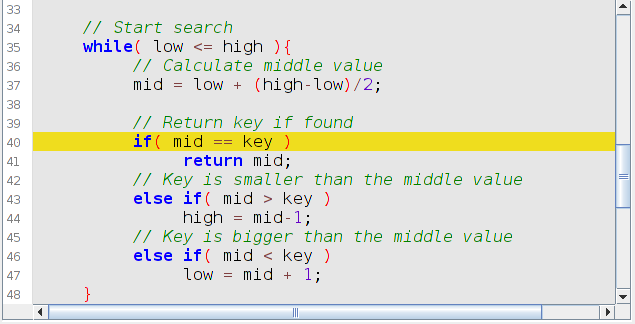
\includegraphics[width=0.7\textwidth]{./media/images/gui/main/CCompact-gui-left-code-2.png}
  \caption{Das Textfeld für den Sourcecode}
  \label{fig:gui-main-left-code}
\end{figure}

Die Zeile, in der sich der Cursor befindet, wird durch einen farbigen Balken markiert. Dieser Balken hat, je nach Modus des Debuggers, die selbe Farbe wie das Zustandspanel (siehe Abbildung \ref{fig:gui-main-left-code}).

Dieses Textfeld wird mit der statischen Methode \textbf{initCodePane()} der Klasse \textbf{InitLeftPanel} initialisiert. Die Methode wird beim Erstellen des linken Teils der Benutzeroberfläche aufgerufen.

\subsection{Ein- und Ausgabetextfeld}
\label{sec:gui-main-left-io}

Im Eingabefeld werden Daten eingegeben, die eingelesen werden, während der Debugger das Programm des Benutzers ausführt. Jedes Zeichen kann nur einmal eingelesen werden; bereits eingelesene Zeichen werden gelb hinterlegt (Abbildung \ref{fig:gui-main-left-io}). Die Ausgabedaten werden in einem separaten Textfeld dargestellt.

\begin{figure}[h!] 
  \centering
     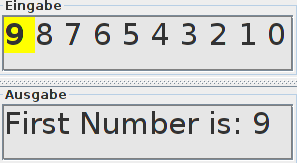
\includegraphics[width=0.4\textwidth]{./media/images/gui/main/io.png}
  \caption{Eingabedaten werden eingelesen, Ausgabe im Textfeld darunter}
  \label{fig:gui-main-left-io}
\end{figure}

In C Compact gibt es für Ein- und Ausgabe keine Konsole, wie sie bei einfachen Programmen meist verwendet wird. Bei unseren Versuchen (siehe Kapitel \ref{sec:sci-trial-intro}) hat sich gezeigt, dass dies die Schülerinnen und Schüler kaum stört. Besonders beim Entwickeln eines Algorithmus ist diese Methode der Ein- und Ausgabe besonders hilfreich, da die Eingabedaten nicht immer wieder eingegeben werden müssen.

Dem Interpreter muss immer ein Objekt, welches das Interface \textbf{StdInOut} (siehe Kapitel \ref{sec:deb-impl-interfaces}) aus dem Package \textbf{at.jku.ssw.cmm.debugger} implementiert, übergeben werden. In diesem Interface befinden sich Methoden zur Ein- und Ausgabe. Diese Methoden werden vom Debugger aufgerufen, wenn im Programm Anweisungen zur Ein- oder Ausgabe vorkommen.

\begin{lstlisting}[language=JAVA]
public interface StdInOut {
	public char in() throws RunTimeException;
	public void out(char arg0);
}
\end{lstlisting}

Für den Debugger wurde die Ein- und Ausgabe in der Klasse \textbf{IOstream} im Package \textbf{at.jku.ssw.cmm.debugger} implementiert. Die (gekürzte) Programmierung sieht wie folgt aus:

\begin{lstlisting}[language=JAVA]
@Override
public char in() throws RunTimeException {

	char c;
	try {
		// Zeichen lesen und aus der Liste löschen
		c = this.inputStream.get(0);
		this.inputStream.remove(0);
	} catch (Exception e) {
		// Throw interpreter runtime error if no more input data available
		throw new RunTimeException("no input data", null, 0);
	}
	
	// Gelesenes Zeichen im Textfeld markieren
	this.main.getLeftPanel().increaseInputHighlighter();
	
	return c;
}

@Override
public void out(final char arg0) {

	java.awt.EventQueue.invokeLater(new Runnable() {
		public void run() {
			// Zeichen zur Ausgabe hinzufügen
			main.getLeftPanel().outputStream("" + arg0);
		}
	});
}
\end{lstlisting}

Da der Interpreter in einem separaten Thread ausgeführt wird, muss die Ausgabe der übergebenen Daten in den \textbf{Event Dispatcher Thread} eingereiht werden. Für die Eingabedaten ist das nicht notwendig, da der Eingabestring in in einem Feld dieser Klasse gespeichert wird und als \textbf{final} deklariert wurde (siehe Kapitel \ref{sec:deb-impl-thread-problems}).

Für das Textfeld für die Eingabedaten wurde die Klasse \textbf{JInputDataPane} erstellt. Diese Klasse erbt von \textbf{JTextPane}\footnote{http://docs.oracle.com/javase/7/docs/api/javax/swing/JTextPane.html}. Die Klasse JInputDataPane ist im Package \textbf{at.jku.ssw.cmm.gui.init} zu finden. 
%TODO TODO beschreiben, wozu JInputTextPane da ist?

Die Textfelder werden mit den statischen Methoden \textbf{initInputPane()} und \textbf{initOutputPane()} der Klasse \textbf{InitLeftPanel} initialisiert.

\section{Rechter Teil der Benutzeroberfläche}
Der rechte Teil der Benutzeroberfläche besteht aus einem Zustandspanel für die aktuelle Aufgabe (Quest) und einem Panel mit mehreren Registerkarten, die unterschiedliche Bedienelemente enthalten, zum Beispiel für den Debugger.

Ähnlich wie der linke Teil der Benutzeroberfläche wird auch dieser Bereich von einer eigenen Klasse verwaltet. Die Klasse \textbf{GUIrightPanel} im Package \textbf{at.jku.ssw.cmm.gui} bildet eine Schnittstelle zwischen dem Hauptteil der Benutzeroberfläche (der Klasse \textbf{GUImain}, siehe Kapitel \ref{gui-main}) und den Komponenten, die in den Registerkarten des rechten Panels eingebettet sind.

Wie bei der Klasse \textbf{GUIleftPanel} wird die Benutzeroberfläche dieses Bereiches mit der Methode \textbf{init} erstellt. Als Parameter wird eine Referenz auf \textbf{GUImain} übergeben, der Rückgabewert ist das fertig initialisierte rechte Panel.

In den Registerkarten können folgende Inhalte vorhanden sein:
\def\arraystretch{1.6}
\begin{table}[h!]
\begin{tabular}{|l|p{2.5cm}|p{6.6cm}|l|}
\hline
\textbf{Name}&\textbf{Sichtbar}&\textbf{Beschreibung}&\textbf{Siehe Kapitel}\\
\hline
Debug&Immer&Enthält Elemente zum Bedienen des Debuggers&\ref{sec:deb-use}\\
Error&Fehler aufgetreten&Zeigt detaillierte Informationen zu einem Fehler an&\ref{sec:deb-error}\\
Quest&Questsystem aktiv&Zeigt die aktuelle Aufgabenstellung an und ermöglicht das Überprüfen der Aufgabe&0.0.0\\ %TODO ref Questsystem (instead of 0.0.0)
Profile&Questsystem aktiv&Zeigt das Profil des Benutzers: Benutzerbild, Name und Auszeichnungen&0.0.0\\ %TODO ref Profile, profilePanel (instead of 0.0.0)
\hline
\end{tabular}
\caption{Registerkarten im rechten Teil des Hauptfensters}\label{tab:gui-main-right-reg}
\end{table}

\subsection{Zustandspanel des Questsystems}
Dieses Zustandspanel visualisiert den aktuellen Status des Questsystems und ist daher auch nur gemeinsam mit diesem verfügbar (in Kapitel \ref{sec:gui-main-impl} wurde dargelegt, wie C Compact ohne den Funktionen des Questsystems gestartet werden kann). Die Zustände des Questsystems sind vollkommen unabhängig von denen des Debuggers.
%TODO ref quest system, quest tester

Folgende Zustände können angezeigt werden:
\begin{enumerate}
\item \textbf{Keine Quest ausgewählt (Idle):} Zu Beginn hat der Benutzer noch keine Aufgabe ausgewählt, das Zustandspanel ist grau.
\item \textbf{Quest wird bearbeitet:} Während der Benutzer eine ausgewählte Aufgabe bearbeitet, ist das Panel blau.
\item \textbf{Quest wird getestet:} Wenn der Benutzer überprüfen will, ob er eine Aufgabe richtig erfüllt hat, startet er einen Test. Während des Tests wird das Zustandspanel gelb, im Regelfall ist dieser Status aber sehr kurz. Wenn während des Tests ein Fehler auftritt (wie etwa eine Endlosschleife), kann der Test in diesem Zustand abgebrochen werden.
%TODO ref Quest test, quest test panel
\item \textbf{Test erfolgreich:} Verläuft der Test erfolgreich, wird das Zustandspanel grün.
\item \textbf{Test fehlgeschlagen:} In diesem Fall ist entweder ein Fehler im Sourcecode des Benutzers erkannt worden (eine detaillierte Beschreibung wird im Fehlerpanel angezeigt, siehe Kapitel \ref{sec:deb-error}) oder das Programm des Benutzers erfüllt die gestellte Aufgabe nicht.
\end{enumerate}

Der angezeigte Zustand wird mit folgenden Methoden der Klasse \textbf{GUIrightPanel} initialisiert. Diese Methoden sind wirkungslos, wenn das Questsystem deaktiviert ist.
\begin{lstlisting}[language=JAVA]
public void setIdleMode();
public void setQuestMode(String title);
public void setTestMode();
public void setSuccessMode();
public void setFailedMode();
\end{lstlisting}

\subsection{Registerkarte \glqq{}Debug\grqq{}}
\label{sec:gui-main-right-reg-deb}
Diese Registerkarte ist immer die erste in der Reihenfolge der Tabs und ist jederzeit verfügbar. Im oberen Teil befindet sich ein Panel mit Bedienelementen des Debuggers, darunter werden die Variablen im Programm des Benutzers während der Laufzeit des Interpreters dargestellt (siehe Kapitel \ref{sec:deb-idea}).

Eine Referenz auf das Panel in dieser Registerkarte wird von folgender Methode übergeben:
\begin{lstlisting}[language=JAVA]
public GUIdebugPanel getDebugPanel() {
	return this.debugPanel;
}
\end{lstlisting}

\subsection{Registerkarte \glqq{}Error\grqq{}}
\label{sec:gui-main-right-error}
Wenn beim Debuggen ein Fehler im Compiler, Präprozessor oder Interpreter auftritt, wird dieses Panel sichtbar. Fehler im Quelltext des Benutzers, die beim Überprüfen einer Quest bemerkt werden, werden ebenfalls hier angezeigt. Ist der Fehler behoben und wurde das Programm erfolgreich ausgeführt, verschwindet diese Registerkarte automatisch.

Mit folgender Methode werden Fehlernachrichten eingeblendet. Als Parameter wird die Fehlernachricht des Compiler, Präprozessor oder Interpreter übergeben. Der Rückgabewert ist der Name (Präfix und Postfix) des Fehlers, wie er im Zustandspanel des Debuggers angezeigt wird. Siehe dazu Kapitel \ref{sec:gui-main-left-zust}.%TODO also ref debugger:states
\begin{lstlisting}[language=JAVA]
public String[] showErrorPanel(String errorCode);
\end{lstlisting}

Eine detaillierte Beschreibung zu der Verwaltung von Fehlerdokumenten ist in Kapitel \ref{sec:deb-error} zu finden.

\subsection{Registerkarte \glqq{}Quest\grqq{}}
In dieser Registerkarte werden Informationen und Bedienelemente zum Ausführen einer Aufgabe des Questsystems (siehe Kapitel \ref{sec:deb-error}) angezeigt.

Eine Referenz auf das Panel in dieser Registerkarte wird von folgender Methode übergeben:
\begin{lstlisting}[language=JAVA]
public GUITestPanel getTestPanel(){
	return this.testPanel;
}
\end{lstlisting}

%TODO also mention this in chapter "quest panel"
Anmerkung: Dieses Panel wird - vor allem im Sourcecode von C Compact - auch als \glqq{}testPanel\grqq{} bezeichnet, da der Benutzer mit Elementen dieses Komponenten überprüfen kann, ob er die aktuelle Aufgabe richtig gelöst hat.

\subsection{Registerkarte \glqq{}Profile\grqq{}}
Hier werden Informationen zum aktuellen Spielerprofil angezeigt. Siehe Kapitel \ref{}.
%TODO ref

Eine Referenz auf das Panel in dieser Registerkarte wird von folgender Methode übergeben:
\begin{lstlisting}[language=JAVA]
public ProfilePanel2 getProfilePanel() {
	return this.questPanel;
}
\end{lstlisting}

\section{Menüleiste}
\label{sec:gui-main-menu}
Menüs sind bei der Gestaltung einer Benutzeroberfläche nahezu unerlässlich. Eine Menüleiste, bzw. ein Menü erleichtert dem Benutzer die Orientierung, da alle Funktionen auf einen Blick zu finden sind. Die Menüleiste wird auch in den \emph{Common User Access}\footnote{http://de.wikipedia.org/wiki/Common\_User\_Access} Richtlinien für die Gestaltung von Benutzeroberflächen definiert; diese Standards wurden 1989 von der Firma IBM festgelegt. Sie sind mittlerweile weit verbreitet und wurden in einer Reihe von Systemen umgesetzt.

Die Menüleiste wird in der statischen Methode \textbf{initFileM()} in der Klasse \\ \textbf{at.jku.ssw.cmm.gui.init.InitMenuBar} angelegt. Die Tastaturkürzel - \emph{\glqq{}Keyboard Shortcuts\grqq{}} - zum Beispiel \emph{Strg + S} zum Speichern, werden ebenfalls hier definiert. Beim Verwenden eines Tastaturkürzels wird der Event Listener des zugehörigen Menüeintrages aufgerufen.
%TODO ref to keyboard shortcuts in GUIcontrolPanel

Initialisieren eines Menüeintrages:
\begin{lstlisting}[language=JAVA]
// Menüeintrag wird initialisiert
JMenuItem openMI = new JMenuItem(_("Open"));

// Menüeintrag wird zum Menü hinzugefügt
fileM.add(openMI);

// Mit dem Action Listener verknüpfen, sodass dieser beim Anklicken des Menüs aufgerufen wird
openMI.addActionListener(listener.openHandler);

// Mit dem Keyboard Shortcut verknüpfen
openMI.setAccelerator(KeyStroke.getKeyStroke(KeyEvent.VK_O, ActionEvent.CTRL_MASK));

// Eintrag zur MenuBarControl hinzufügen
menuBarControl.add(newMI);
\end{lstlisting}

Die Events der Menüleiste werden in der Klasse \textbf{MenuBarEventListener} im Paket \textbf{at.jku.ssw.cmm.gui.event} abgewickelt. Diese Klasse enthält Methoden, die bestimmte Aktionen ausführen und innere Klassen, die einen Event Listener implementieren und diese Methoden aufrufen. Diese Aufteilung ist nötig, da bestimmte Aktionen auch von anderen Instanzen aufgerufen werden können (zum Beispiel wird auch gespeichert, wenn der Benutzer C Compact schließt).

\subsection{Aktivieren und Deaktivieren von Menüeinträgen}
\label{sec:gui-main-menu-ctrl}
Da während der Debugger ausgeführt wird keine Aktionen erlaubt sind, die den Text im Sourcecode Textfeld ändern (siehe Kapitel \ref{sec:gui-main-left-code}), werden bestimmte Menüeinträge aktiviert oder deaktiviert, wenn sich der Status des Debuggers ändert (Siehe Kapitel \ref{sec:gui-main-left-zust}). Diese Aktionen werden in der Klasse \textbf{at.jku.ssw.cmm.gui.MenuBarControl} zusammengefasst. Diese Klasse enthält eine Liste, in der alle Menüeinträge referenziert werden, die beim Ausführen des Debuggers deaktiviert werden sollen. Mit der Methode \textbf{add()} werden Objekte in diese Liste eingetragen.
\begin{lstlisting}[language=JAVA]
public void add(JMenuItem mi){
	this.list.add(mi);
}
\end{lstlisting}

Mit den Methoden \textbf{lockAll()} und \textbf{unlockAll()} werden diese Menüeinträge dann deaktiviert oder aktiviert.

\begin{lstlisting}[language=JAVA]
public void lockAll();
public void unlockAll();
\end{lstlisting}

Des Weiteren kann in dieser Kontrollklasse ein Menüeintrag definiert werden, der eine Liste der zuletzt geöffneten Dateien enthält. Mit der Methode \textbf{setRecentMenu} wird dieser Menüeintrag definiert:
\begin{lstlisting}[language=JAVA]
public void setRecentMenu( JMenu mi ){
	this.recentMI = mi;
}
\end{lstlisting}

Dieses Untermenü wird mit der Methode \textbf{updateRecentFiles} aktualisiert.
\begin{lstlisting}[language=JAVA]
public void updateRecentFiles( List<String> recentFiles, String currentFile );
\end{lstlisting}

Im Untermenü \glqq{}Sourcecode\grqq{} (siehe Kapitel \ref{sec:gui-menu-code}) gibt es Funktionen zum Aufheben bzw. Wiederholen der letzten Aktion (\emph{undo and redo}). Diese Menüeinträge sollen aber nur aktiviert sein, wenn eine solche Aktion tatsächlich möglich ist. Beispielsweise kann nach dem Start des Programmes nichts rückgängig gemacht werden, da noch keine Aktionen durchgeführt wurden. Außerdem dürfen diese Aktionen nicht ausgeführt werden, wenn der Debugger gerade läuft, da der Sourcecode sonst während der Laufzeit verändert werden würde.

Referenzen auf die beiden entsprechenden Menüeinträge werden in der Klasse MenuBarControl separat gespeichert.
\begin{lstlisting}[language=JAVA]
public void setUndo(JMenuItem undo){
	this.undo = undo;
}

public void setRedo(JMenuItem redo){
	this.redo = redo;
}
\end{lstlisting}

Mit der Methode \textbf{updateUndoRedo()} werden die Zustände dieser Menüeinträge aktualisiert. Als Parameter werden eine Referenz auf das Textfeld mit dem Sourcecode und eine boolean-Variable übergeben. Letztere ist \textbf{true} wenn der Debugger gerade läuft.
\begin{lstlisting}[language=JAVA]
public void updateUndoRedo( RSyntaxTextArea tArea, boolean running ){
	this.undo.setEnabled(!running & tArea.canUndo());
	this.redo.setEnabled(!running & tArea.canRedo());
}
\end{lstlisting}

\subsection{Menü \glqq{}Datei\grqq{}}
\label{sec:gui-main-menu-file}
Das wohl bekannteste Menü in jedem Programm ist das Menü \glqq{}Datei\grqq{}. In C Compact enthält es neben den grundlegenden Funktionen zum Öffnen oder Speichern einer vorhandenen oder neuen Datei auch noch weitere Funktionen. Der Eintrag \glqq{}Drucken\grqq{} verwendet eine Methode, die in der RSyntaxTextArea implementiert ist (siehe Kapitel \ref{sec:gui-main-left-code}; allerdings treten bei der Formatierung oft Fehler auf. Wesentlich wichtiger sind die Menüpunkte \glqq{}Einstellungen\grqq{} (siehe Kapitel \ref{sec:win-set}), \glqq{}Sprache\grqq{} (siehe Kapitel \ref{sec:win-lang}) und \glqq{}Über C Compact\grqq{} (siehe Kapitel \ref{sec:win-credits}). Schließlich gibt es noch dem Menüpunkt \glqq{}Beenden\grqq{}, C Compact kann aber auch mit der Tastenkombination \emph{Alt + F4} (diese Kombination ist in den meisten Betriebssystemen und Oberflächen bereits standardmäßig verwendet) oder über entsprechende Bedienelemente im Fensterrahmen geschlossen werden.

\subsection{Menü \glqq{}Sourcecode\grqq{}}
\label{sec:gui-menu-code}
Dieses Menü würde in den meisten Programmen dem Menü \glqq{}Bearbeiten\grqq{} entsprechen. Allerdings beziehen sich die Menüeinträge wie \glqq{}Kopieren\grqq{}, \glqq{}Einfügen\grqq{}, \glqq{}Rückgängig\grqq{}, etc. immer auf das Textfeld für den Sourcecode --- mit dem Menünamen sollen also Verwechslungen vermieden werden --- und andererseits enthält dieses Menü auch Einträge zum Steuern des Debuggers. Diese Einträge werden vom Benutzer kognitiv mit dem Sourcecode verknüpft.

\subsection{Menü \glqq{}Fortschritt\grqq{}}
Dieses Menü enthält Einträge, die das Questsystem (siehe Kapitel \ref{}) betreffen. Mit \glqq{}Profil Wählen\grqq{} Wird C Compact beendet und der Launcher (siehe Kapitel \ref{}) gestartet, sodass der Benutzer ein anderes Profil wählen kann. Mit dem Befehl \glqq{}Profil Exportieren\grqq{} kann der Benutzer sein Profil an einem anderen Ort speichern (siehe Kapitel \ref{}). Der Menüeintrag \glqq{}Quest wählen\grqq{} öffnet ein Fenster zum Auswählen eines Questpaketes; im Anschluss kann der Benutzer eine Aufgabe zum Bearbeiten wählen (siehe Kapitel \ref{}). Mit \glqq{}Questpaket importieren\grqq{} kann ein Package importiert werden (siehe Kapitel \ref{} und \ref{}).
%TODO ref Questsystem
%TODO ref launcher
%TODO ref profil exportieren
%TODO ref select quest window
%TODO ref package, import package


	%!TEX root = "../../../DA_GUI.tex"

%	--------------------------------------------------------
% 	Funktionsweise des Debuggers
%	--------------------------------------------------------

\chapter{Der Debugger}

%   Einleitung
%!TEX root = "../../../DA_GUI.tex"

%	--------------------------------------------------------
% 	Debugger: Einleitung
%	--------------------------------------------------------

\section{Einleitung}

%   --------------------------------------------------------
%   Grundlegende Funktionen, Ideen
%   --------------------------------------------------------

\subsection{Die grundlegende Idee}
\label{sec:deb-idea}
Ein wichtiger Bestandteil von C Compact ist der integrierte Debugger, der speziell für die Bedürfnisse von Anfängern ausgelegt ist. Während das Programm Schritt für Schritt abgearbeitet wird, sind alle Variablen und der Call Stack in übersichtlicher Form dargestellt. In der Variablentabelle werden Wertänderungen farbig hervorgehoben. Dadurch soll ein fundiertes Verständnis für den Programmablauf und die Logik dahinter entstehen.

\begin{figure}[h]
\centering
\includegraphics[width=0.7\textwidth]{./media/images/gui/debugger/gui-debugger-marked.png}
\caption{Die vier Komponenten des Debuggers}
\label{fig:deb-intro-m1}
\end{figure}

Während die Debugger professioneller Entwicklungsumgebungen eine Hilfestellung für erfahrene Programmierer sind, ist der Debugmodus von C Compact besonders auf Anfänger ausgelegt. Damit Einsteiger und unerfahrene Programmierer von Beginn an mit dem Debugger in Berührung kommen, ist er ein fester Bestandteil der Benutezroberfläche.

Abbildung \ref{fig:deb-intro-m1} zeigt die vier Komponenten des Debuggers in der Benutzeroberfläche:
\begin{enumerate}
\item Im Quelltext wird die gerade abgearbeitete Zeile markiert
\item Mit den Kontrollelementen kann der Debugger gestartet und angehalten werden
\item Die Variablen des Programms werden übersichtlich angezeigt
\item Ein- und Ausgabe des laufenden Programms befinden sich in getrennten Textfeldern, eingelesene Zeichen werden gelb markiert.
\end{enumerate}

%   --------------------------------------------------------
%   Bedienung des Debuggers
%   --------------------------------------------------------

\subsection{Bedienung des Debuggers}
\label{sec:deb-use}
Mit den Kontrollelementen kann der Debugger intuitiv und einfach bedient werden. Die Bedienelemente (Abbildung \ref{fig:deb-gui-ctrl}) sind im rechten Teil des Hauptfensters im Tab \glqq{}Debug\grqq{} (siehe Kapitel \ref{sec:gui-main-right-reg-deb}) zu finden.

\def\arraystretch{1.4}
\begin{table}[h]
\begin{tabular}{|l|l|l|l|}
	\hline
	Element & \parbox{2cm}{Keyboard\\Shortcut}& Name & Funktion\\
	\hline
	\ding{228} / \ding{122}\thinspace \ding{122} & F5 & Play/Pause & Startet den Debugger/Hält den Debugger an\\
	\ding{122}\thinspace \ding{228} & F6 & Step & Springt zum nächsten Schritt weiter\\
	\ding{110} & F7 & Stop & Beendet den Debugger\\
	--- & --- & Schieberegler & \parbox{7cm}{Ändert die Zeitabstände beim automatischen Debuggen}\\
	\hline
\end{tabular}
\caption{Funktionen der Bedienelemente des Debuggers}\label{tab:deb-ctrl}
\end{table}



\begin{figure}[h]
\centering
\includegraphics[width=0.4\textwidth]{./media/images/gui/debugger/ctrl-elements.png}
\caption{Kontrollelemente des Debuggers}
\label{fig:deb-gui-ctrl}
\end{figure}

Der Debugger hat vier unterschiedliche Modi, die im linken Teil des Hauptfensters durch eine Zustandsanzeige visualisiert werden (siehe Kapitel \ref{sec:gui-main-left-zust}). Der Wechsel zwischen diesen Zuständen erfolgt durch Eingaben des Benutzers, entweder mit den Kontrollelementen (Buttons) in der Benutzeroberfläche, oder mit Keyboard Shortcuts.
%TODO ref keyboard shortcuts

Die vier Zustände sind:
\begin{enumerate}
\item \textbf{Text bearbeiten (ready mode)}
Dies ist der Standardzustand. Der Quelltext und Eingabedaten für den Debugger können bearbeitet werden. Außerdem sind Dateioperationen erlaubt.
\begin{figure}[h!]
\centering
\includegraphics[width=0.65\textwidth]{./media/images/gui/debugger/mode-idle.png}
\caption{Zustandsanzeige für den Editormodus}
\label{fig:deb-zust-1}
\end{figure}
\item \textbf{Fehler aufgetreten (error mode)}
Beim Compilieren oder während der Laufzeit des Debuggers ist ein Fehler aufgetreten. Um diesen zu beheben, ist das Bearbeiten des Quelltexts nach wie vor erlaubt.
\begin{figure}[h!]
\centering
\includegraphics[width=0.65\textwidth]{./media/images/gui/debugger/mode-error.png}
\caption{Zustandsanzeige für den Fehlermodus}
\label{fig:deb-zust-2}
\end{figure}
\item \textbf{Programm Schritt für Schritt abarbeiten oder Pause (pause mode)}
Der Debugger ist aktiv, wartet aber auf eine Eingabe des Benutzers, um den nächsten Befehl abzuarbeiten. In diesem Modus kann der Benutzer sein Programm Schritt für Schritt abarbeiten. Das Modifizieren des Quelltextes ist in diesem Modus nicht möglich.
\begin{figure}[h!]
\centering
\includegraphics[width=0.65\textwidth]{./media/images/gui/debugger/mode-step.png}
\caption{Zustandsanzeige für den Pausemodus}
\label{fig:deb-zust-3}
\end{figure}
\item \textbf{Programm automatisch abarbeiten (run mode)}
Das Programm des Benuters wird Schritt für Schritt abgearbeitet. Zwischen den Befehlen wird für eine bestimmte Zeit zwischen 0 und 5 Sekunden gewartet. Diese Verzögerung kann mit dem Schieberegler bei den Kontrollelementen eingestellt werden. Auch hier kann der Quelltext nicht verändert werden.
\begin{figure}[h!tp]
\centering
\includegraphics[width=0.65\textwidth]{./media/images/gui/debugger/mode-run.png}
\caption{Zustandsanzeige für den Automatischen Debugmodus}
\label{fig:deb-zust-4}
\end{figure}
\end{enumerate}

\begin{figure}[h!]
\centering
\includegraphics[width=0.65\textwidth]{./media/images/gui/debugger/RunModes_Simple.png}
\caption{Vereinfachtes Zustandsdiagramm des Debuggers}
\label{fig:deb-zust-simple}
\end{figure}

%Obwohl der Debugger selbst zwischen Modus Editormodus (1) und Fehlermodus (2) unterscheidet, gibt es in der Benutzeroberfläche nur mehr den Editormodus. Der Fehlermodus wird trotzdem im Zustandspanel des Debuggers im Hauptfenster angezeigt, damit der Benutzer auf den aufgetretenen Fehler aufmerksam gemacht wird. Wie in Abbildung \ref{fig:deb-zust-simple} ersichtlich ist, erfüllen die beiden Modi die selben Funktionen.

Der Pausemodus (3) hat zwei Funktionen: einerseits entspricht dieser Modus einer Pausierung (bezogen auf Zustand 4, in dem der Debugger automatisch durchläuft) und andererseits kann in diesem Modus mit dem \glqq{}Nächster Schritt\grqq{} Button auch direkt zum nächsten Befehl gesprungen werden.

Ein Sonderfall des run mode ist der \glqq{}quick run mode\grqq{}. Wenn der Regler für die Zeitabstände zwischen den Schritten des Debuggers auf null gestellt wird, werden die folgenden Schritte so schnell wie möglich abgearbeitet, bis entweder das Programm zu Ende ist oder der Debugger auf einen \glqq{}wait\grqq{}-Befehl stößt.

%   --------------------------------------------------------
%   Schlüsselwörter
%   --------------------------------------------------------

\subsection{Schlüsselwörter}
\label{sec:deb-keywords}
%TODO ref compiler
In der Sprache von C Compact gibt es zwei spezielle Schlüsselwörter, die Einfluss auf das Verhalten des Debuggers nehmen: \textbf{wait} und \textbf{library}.

\subsubsection*{wait}
%TODO ref AST
In C Compact gibt es seit der Version Alpha 1.2 keine Breakpoints als Option in der Benutzeroberfläche mehr. Anstatt dessen wird der Befehl \textbf{wait} verwendet. Dieser Befehl kann in jeder Funktion verwendet werden. Stößt der Debugger auf diesen Befehl, geht er in den \textbf{Pausemodus}. An dieser Stelle kann der Debugger dann entweder Schritt für Schritt, oder wieder im automatischen Debugmodus fortgesetzt werden.

\begin{lstlisting}[language=CMM]
wait;
\end{lstlisting}

Durch die Umsetzung der Breakpoint-Funktion als Befehl in der Sprache besteht immer ein klarer Zusammenhang zwischen Aktionen des Debuggers und dem Quelltext.

\subsubsection*{library}
Funktionen und Variablen können vor dem Debugger \glqq{}versteckt\grqq{} werden. Das Attribut \textbf{library} kann sowohl für eine Variable, als auch für eine Funktion verwendet werden. Das Schlüsselwort muss immer zwischen Typ und Name der Variable bzw. Funktion stehen.

\begin{lstlisting}[language=CMM]
const float library M_PI = 3.141592654;
\end{lstlisting}
Eine Variable mit dem \textbf{library}-Attribut wird im Debugger nicht angezeigt. Dies wird zum Beispiel verwendet, um die zahlreichen Konstanten der Bibliothek \textbf{math.h} im Debugger auszublenden.

\begin{lstlisting}[language=CMM]
float library sin(float x);
\end{lstlisting}
Hat eine Funktion das \textbf{library}-Attribut, springt der Debugger nicht in diese Funktion, sondern arbeitet sie in einem Schritt ab. Dadurch können Bibliotheksfunktionen im Debugger als einzelner Befehl in einem Schritt abgearbeitet werden.


%   Implementierung
%!TEX root = "../../../DA_GUI.tex"

%	--------------------------------------------------------
% 	Debugger: Implementierung
%	--------------------------------------------------------

\section{Implementierung}

%   --------------------------------------------------------
%   Interfaces
%   --------------------------------------------------------

\subsection{Interfaces}
\label{sec:deb-impl-interfaces}
Für die Kommunikation mit dem Interpreter sind zwei Interfaces wichtig. Im Package \textbf{at.jku.ssw.cmm.debugger} befinden sich das Interface \textbf{Debugger} und das Interface \textbf{StdInOut}. Die benötigten Methoden sind in zwei Interfaces aufgeteilt, da sie unterschiedliche Teile der Benutzeroberfläche betreffen. Bei einfacheren Anwendungen des Interpreters, wie etwa beim Testen von Quests, werden beide Interfaces in der selben Klasse implelemtiert.
%TODO ref quest test

Über das Interface \textbf{Debugger} übergibt der Interpreter jeweils den aktuellen Knoten im abstrakten Syntaxbaum. In der Methode \textbf{step} werden außerdem eine Liste der Variablen, die im letzten Schritt ausgelesen wurden und eine Liste der Variablen, die im letzten Schritt geändert wurden übergeben. Die geänderten Variablen werden in der Variablenliste im Hauptfenster gelb markiert. Es ist möglich, dass in einem Schritt mehrere Variablen geändert werden, da mit dem Befehl \textbf{library} eine ganze Funktion auf einmal abgearbeitet werden kann.

\begin{lstlisting}[language=JAVA]
public interface Debugger {
	boolean step(Node arg0, List<Integer> readVariables, List<Integer> changedVariables);
}
\end{lstlisting}

Die Methode \textbf{step} muss \textbf{true} zurückgeben, ansonsten bricht der Interpreter ab. Auf diese Weise kann der Interpreter beendet werden.

Das Interface \textbf{StdInOut} enthält Methoden zur Ein- und Ausgabe im Programm. Die Methode \textbf{in} kann eine \textbf{RunTimeException} verursachen, um den Interpreter anzuhalten, wenn keine Eingabedaten vorhanden sind. Die Methode \textbf{out} übergibt das Zeichen, das ausgegeben werden soll. Siehe auch Kapitel \ref{sec:gui-main-left-io}.

\begin{lstlisting}[language=JAVA]
public interface StdInOut {
	public char in() throws RunTimeException;
	public void out(char arg0);
}
\end{lstlisting}

%   --------------------------------------------------------
%   Starten des Threads
%   --------------------------------------------------------

\subsection{Der Thread des Debuggers}
Alle Aktionen der Benutzeroberfläche werden im sogenannten Event Dispatch Thread\footnote{https://docs.oracle.com/javase/tutorial/uiswing/concurrency/dispatch.html} (auch EDT) ausgeführt. Wenn dieser Thread angehalten wird, kann die Benutzeroberfläche nicht mehr auf Eingaben des Benutzers reagieren. Der Debugger soll aber jederzeit verzögert werden können. Deshalb wird der Interpreter in einem eigenen Thread ausgeführt.

Die Klasse \textbf{CMMwrapper} im Package \textbf{at.jku.ssw.cmm} enthält Methoden zum Starten des Threads und sorgt außerdem dafür, dass nicht mehrere Threads gleichzeitig ausgeführt werden.

Der Interpreter wird mit folgender Methode in einem eigenen Thread gestartet:
\begin{lstlisting}[language=JAVA]
public boolean runInterpreter(PanelRunListener listener, IOstream stream, Tab table) {

	// Check if another interpreter thread is already running
	if ( table != null && this.thread == null ) {
			
		this.table = table;

		// Reset the output text panel
		this.main.getLeftPanel().resetOutputTextPane();

		this.interpreter = new Interpreter(listener, stream);

		// Create new interpreter object
		this.thread = new CMMrun(table, interpreter, this, debug);

		// Run interpreter thread
		this.thread.start();

		return true;
	}
	// Another thread is already running
	else {
		// Error message
		DebugShell.out(State.ERROR, Area.INTERPRETER, "Already running or not compiled!");

		return false;
	}
}
\end{lstlisting}

Die Variable \textbf{thread} der Klasse \textbf{CMMwrapper} ist eine Referenz auf den aktuell laufenden Interpreter-Thread. Wenn diese Variable nicht \textbf{null} ist, bedeuted das, dass bereits ein anderer Thread läuft. Wenn der Thread des Interpreters richtig beendet wird, ruft er die Methode \textbf{setNotRunning()} auf. Die Referenz auf diesen Thread wird gelöscht und ein neuer Thread kann bei bedarf gestartet werden.
\begin{lstlisting}[language=JAVA]
public void setNotRunning() {
	this.thread = null;
}
\end{lstlisting}

%TODO keep code ref up to date
Die Klasse \textbf{CMMrun} erbt von der Klasse Thread\footnote{https://docs.oracle.com/javase/7/docs/api/java/lang/Thread.html}. Ein neuer Thread wird gestartet, indem die Methode \textbf{start()}, die von der Klasse Thread vererbt wurde, aufgerufen wird (siehe erstes Codebeispiel dieses Abschnitts, Zeile 17). Der Thread führt dann die Methode \textbf{run()} aus, die ebenfalls vererbt wird und in der Kindklasse überschrieben werden muss.
\begin{lstlisting}[language=JAVA]
@Override
public void run() {

	// Allocating memory for interpreter
	Memory.initialize();

	// Run main function
	try {
		interpreter.run(table);
	}
	// Thrown when runtime error occurs
	catch (final RunTimeException e) {
		// Laufzeitfehler abfangen
		... 
		reply.setNotRunning();
		return;
	} catch (Exception e) {
		// Unerwartete Fehler abfangen
		...
		reply.setNotRunning();
		return;
	}

	// Thread freigeben, sodass ein neuer thread gestartet werden kann
	reply.setNotRunning();
}
\end{lstlisting}

Ein Thread wird beendet, indem die Methode \textbf{run} verlassen wird. Dies ist die einfachste und sicherste Möglichkeit einen Thread zu stoppen. Wenn der Thread von Außen beendet wird, kann nicht sichergestellt werden, dass er zu dieser Zeit nicht gerade auf eine Variable zugreift und durch den Abbruch einen Schreibprozess nicht abschließen kann.

\subsection{Probleme beim Arbeiten mit Threads}
\label{sec:deb-impl-thread-problems}
Das Verwenden mehrerer Threads erfordert generell Vorsicht; vor Allem wenn eine Variable oder eine Referenz von mehreren Threads verwendet wird können unerwartete Komplikationen auftreten.

%TODO ref "Sprechen Sie Java?"
Auf eine Datenstruktur oder Variable sollte immer nur ein Thread gleichzeitig zugreifen können. Da die Wechsel zwischen Threads praktisch nicht vorhersehbar sind, ist es bei unvorsichtiger Implementierung möglich, dass mehrere Threads gleichzeitig auf einem Speicherplatz schreiben oder lesen (Threadinterferenz). Im schlimmsten Fall führt dies zu Exceptions und Abstürzen, deren Ursache dann meistens schwer nachvollziehbar ist.

Es kann auch vorkommen, dass ein Thread eine Variable ausliest, bevor sie durch einen anderen Thread aktualisiert wurde (Speicherinkonsistenz\footnote{https://docs.oracle.com/javase/tutorial/essential/concurrency/memconsist.html}).

Um Variablen und Instanzen in mehreren Threads zu verweden, gibt es --- je nach Anwendungsfall --- unterschiedliche Möglichkeiten:

\subsubsection*{volatile}
Für alle Variablen und Referenzen, die zusätzlich mit dem Schlüsselwort $\textbf{volatile}\footnote{https://docs.oracle.com/javase/tutorial/essential/concurrency/atomic.html}$ deklariert werden, werden Lese- und Schreibvorgänge in einem Schritt ausgeführt (die Operation ist nicht unterbrechbar, also atomar\footnote{http://www.angelikalanger.com/Articles/EffectiveJava/42.JMM-volatileIdioms/42.JMM-volatileIdioms.html}). Dadurch werden Threadinterferenzen vermieden, allerdings sind Probleme durch Speicherinkonsistenz immer noch möglich.
Ein Zugriff auf eine mit \textbf{volatile} deklarierte Variable ist dafür schneller als ein Zugriff über eine \textbf{synchronzied}-Methode (siehe unten).

\begin{lstlisting}[language=JAVA]
volatile double d;
\end{lstlisting}

Bei \textbf{volatile} ist Außerdem zu beachten, dass erstens nur einfache Lese- und Schreibvorgänge atomar sein können (beispielsweise ist eine Inkrementation keine atomare Operation) und sich die atomaren Eigenschaften zweitens nur auf die Variable oder Referenz selbst beziehen, nicht auf das Objekt.

\subsubsection*{final}
Variablen und Referenzen, die als $\textbf{final}$ deklariert werden, können von allen Threads problemlos verwendet werden, da diese Variablen nach dem Initialisieren nicht mehr verändert werden können. Dieses Schlüsselwort wird oft für Funktionsparameter (einfache Wertübergaben) von threadübergreifenden Methoden oder in Kombination mit dem Schlüsselwort \textbf{static} verwendet.

\begin{lstlisting}[language=JAVA]
static final double PI = 3.1415;

public int add( final int a, final int b ) {
	...
}
\end{lstlisting}

Auch \textbf{final} bezieht sich nur auf die Variable oder Referenz selbst. Wird eine Referenz auf ein Objekt \textbf{final} deklariert, können die Variablen des Objektes trotzdem verändert werden.

\begin{lstlisting}[language=JAVA]
final JLabel panel = new JLabel();

// erlaubt
panel.setText("Hello");

// nicht erlaubt
panel = new JLabel("World");
panel = null;
\end{lstlisting}

\subsection*{sychronized}
Für die Kommunikation zwischen Threads ist das Schlüsselwort $\textbf{synchronized}$ unerlässlich. 
\begin{quote}%TODO correct quote
\emph{Synchronized methods enable a simple strategy for preventing thread interference and memory consistency errors: if an object is visible to more than one thread, all reads or writes to that object's variables are done through synchronized methods}
\begin{flushright}Oracle, The Java Turorials\footnote{https://docs.oracle.com/javase/tutorial/essential/concurrency/syncmeth.html}\end{flushright}
\end{quote}
\textbf{synchronized} kann entweder auf eine komplette Methode oder auf einen Programmblock innerhalb einer Methode angewandt werden.

Eine mit \textbf{synchronized} deklarierte Methode wird immer abgeschlossen, bevor eine andere \textbf{synchronized}-Methode dieser Klasse abgearbeitet werden kann. Es wird also sichergestellt, dass keine gleichzeitigen Zugriffe erfolgen.
\begin{lstlisting}[language=JAVA]
public synchronized void setLength(int l){
	this.length = l;
}

public synchronized int getLength() {
	return this.length;
}
\end{lstlisting}

Insbesondere bei umfangreicheren Methoden ist es aber überlegenswert, nur einen Teil der Methode als \textbf{synchronized} zu definieren\footnote{https://docs.oracle.com/javase/tutorial/essential/concurrency/locksync.html}.
\begin{lstlisting}[language=JAVA]
public void doSomething() {
	
	// Ein paar Befehle
	...
	
	synchronized(this) {
		// Einige geschützte Befehle
		...
	}
}
\end{lstlisting}

Dem \textbf{synchronized}-Block muss ein sogenanntes \glqq{}Monitor Object\grqq{} übergeben werden. Dieses Objekt fungiert als \glqq{}Lock\grqq{} (Schloss) für diesen \textbf{synchronized}-Block. Ein Thread erhält nur über dieses Objekt Zugriff auf einen geschützten Block. Will ein anderer Thread auf diesen Block zugreifen, muss er warten, bis das \glqq{}Schloss\grqq{} freigegeben ist.

Grundsätzlich kann jedes beliebige Objekt diese Funktion übernehmen; in den meisten Fällen bietet sich aber \textbf{this} an, da dies auch von \textbf{synchronized}-Mothoden verwendet wird. Werden verschiedene Lock-Objekte verwendet, können diese auch gleichzeitig vergeben werden --- Zugriffe durch mehrere Threads sind dann wieder möglich.

\subsection{Mehrere Threads in Swing}

Objekte, die Teile der Benutzeroberfläche sind, sollten niemals von einem anderen Thread  als dem EDT aus initialisiert oder verändert werden. Dies betrifft Objekte und Instanzen von Klassen aus der AWT- oder Swing-Bibliothek oder daraus abgeleiteten Klassen.%TODO dat grammatics

Um von einem anderen Thread aus ein Swing-Objekt zu verändern, muss dieser Teil des Quellcodes in den Event Dispatch Thread eingereiht werden. Dafür gibt es zwei Möglichkeiten:

\subsubsection*{Asynchroner Aufruf}
Meistens sollte die Methode \textbf{invokeLater()}\footnote{http://docs.oracle.com/javase/7/docs/api/javax/swing/SwingUtilities.html\#invokeLater\%28java.lang.Runnable\%29} verwendet werden.
\begin{lstlisting}[language=JAVA]
java.awt.EventQueue.invokeLater(new Runnable() {
	public void run() {
		...
	}
});
\end{lstlisting}
	Als Parameter wird der Methode invokeLater() ein Objekt des Interfaces \textbf{Runnable}\footnote{http://docs.oracle.com/javase/7/docs/api/java/lang/Runnable.html} übergeben. Das Interface Runnable wird verwendet, um Instanzen oder Methoden in einem Thread auszuführen. Die Klasse Thread selbst implementiert Runnable ebenfalls. Von Runnable abgeleitete Klassen müssen die Methode \textbf{run()} implementieren.
	
	Bei der Verwendung von invokeLater() wird die Methode run() in die Eventliste des Event Dispatch Threads eingereiht. Wenn alle zuvor registrierten Events abgearbeitet wurden, wird diese Methode ausgeführt. Man spricht hier auch von einem \textbf{asynchronen} Aufruf, da die Methode etwas später aufgerufen wird und der Thread, der diese Methode initialisiert hat, möglicherweise bereits andere Programmteile abarbeitet.
	
	Unter den meisten Umständen ist diese Implementierung geeignet, da der Benutzer den Zeitunterschied zwischen Initialisierung des Runnable-Objektes und Änderung in der Benutzeroberfläche nicht wahrnehmen kann. 
	
\subsection*{Synchroner Aufruf}
Es gibt allerdings auch Anwendungsfälle, die eine \textbf{synchrone} Aktualisierung der Benutzeroberfläche erfordern. Ein Beispiel ist das Textfeld für Eingabedaten im Hauptfenster von C Compact (siehe Kapitel \ref{sec:gui-main-left-io}). Wenn der Debugger sehr schnell mehrere Lesebefehle hintereinander ausführt, können bei asynchroner Aktualisierung der Benutzeroberfläche Probleme auftreten, indem ein weiteres Zeichen abgelesen wird während das vorhergehende noch nicht als gelesen markiert wurde (Speicherinkonsistenz). Deshalb wird das Eingabedatenfeld während des Debuggen immer synchron aktualisiert.
\begin{lstlisting}[language=JAVA]
java.awt.EventQueue.invokeAndWait(new Runnable() {
	public void run() {
		...
	}
});
\end{lstlisting}
	Der Thread, von dem aus das Runnable-Objekt instanziert wurde, wird so lange angehalten, bis die Methode run() ausgeführt wurde.

	Diese Umsetzung erfordert allerdings etwas mehr Vorsicht. Während die Methode invokeLater() ohne Probleme auch im Event Dispatch Thread aufgerufen werden kann, würde ein Aufruf von invokeAndWait() aus dem EDT dazu führen, dass sich der Thread selbst blockiert.
	
	Außerdem können bei einem synchronen Aufruf Probleme auftreten, die auf auf den wartenden Thread rückwirken. Für einen reibungslosen synchronen Aufruf müssen folgende Exceptions abgefangen werden können:

\def\arraystretch{2.1}
\begin{tabular}{|l|l|}
	\hline
	InvocationTargetException & \parbox{7cm}{Ein Fehler tritt beim Ausführen der Methode run() auf}\\
	\hline
	InterruptedException & \parbox{7cm}{Der Event Dispatch Thread wurde unterbrochen}\\
	\hline
\end{tabular}


%   --------------------------------------------------------
%   Abarbeiten von Schritten
%   --------------------------------------------------------

\subsection{Abarbeiten von Knoten im Abstrakten Syntaxbaum}
Die Schnittstelle zwischen Benutzeroberfläche und Interpreter bildet die Klasse \textbf{PanelRunListener} im Package \textbf{at.jku.ssw.cmm.gui.event.debug}. Sie implementiert einerseits das Interface \textbf{Debugger} (siehe Kapitel \ref{sec:deb-impl-interfaces}) zum Ausführen von Schritten des Debuggers, andererseits enthält sie Listener für Bedienelemente des Debuggers und den zugehörigen Hotkeys. Außerdem wird hier festgelegt und gespeichert, in welchem Modus sich der Debugger befindet.
%TODO ref ctrl-elements, mode

%TODO ref interpreter, ast
Die einzelnen Schritte im Abstrakten Syntaxbaum werden mit der Methode \textbf{step()} übergeben. Diese Methode wird vom thread des Interpreters aufgerufen und wie folgt abgearbeitet:

\begin{enumerate}
\item Ist der Knoten ein \textbf{wait}-Befehl, wird der Debugger in den \textbf{Pausemodus} versetzt.
\item Ist der Knoten eine Funktionsrückgabe, wird --- sofern diese Funktion aktiviert ist --- ein Popup im Sourcecode mit dem Rückgabewert angezeigt (siehe Kapitel \ref{sec:deb-popup}).
\item Befindet sich der Debugger im \textbf{Schnelldurchlauf} (minimale Verzögerung), wird der Thread des Interpreters nur eine Millisekunde lang verzögert. Danach wird die Methode verlassen.
\begin{lstlisting}[language=JAVA]
Thread.sleep(1);
\end{lstlisting}
Diese Verzögerung ist notwendig, damit die Benutzeroberfläche zwischen den einzelnen Schritten des Interpreters Zeit hat, auf Events zu reagieren.

\item Aktualisierung der Benutzeroberfläche: Die Tabelle mit den Variablen wird aktualisiert, die aktuelle Zeile im Quelltext wird markiert.
\begin{lstlisting}[language=JAVA]
/* --- Variable table update --- */
this.master.updateVariableTables(Memory.getFramePointer() != this.lastAdress);
this.lastAdress = Memory.getFramePointer();
		
/* --- Highlight the changed variables --- */
for( int i : changedVariables )
	this.master.highlightVariable(i, true);
\end{lstlisting}
\emph{Anmerkung zu Zeile 2:} Wenn bei der Aktualisierungsmethode der Variablentabelle \textbf{true} übergeben wird, wird das gesamte Datenmodell der Tabelle neu aufgebaut. Das ist aber nur notwendig, wenn neue Einträge hinzukommen oder Variablen gelöscht werden (Funktion wird aufgerufen oder geändert, Framepointer hat einen anderen Wert).

\item Thread wartet auf Freigabe zum nächsten Schritt. Befindet sich der Debugger im \textbf{automatischen Debugmodus}, wird vorher ein Timer initialisiert, der den nächsten Schritt nach einiger Zeit von selbst auslöst.
\begin{lstlisting}[language=JAVA]
/* --- Initialize auto-debugging delay timer --- */
if (this.isRunMode() && this.delay > 0) {
	this.timer = new Timer();
	// Start timer
	this.timer.schedule(new TimerTask() {
		@Override
		public void run() {
			if( isRunMode() || isPauseMode() )
				userReply();
		}
	}, (int)(delayScale(delay)*1000) );
}

// Wait until timer runs out or user presses "next step" button
waitForUserReply();
		
this.timer = null;
\end{lstlisting}
Die Methode \textbf{waitForUserReply} hält den Thread des Interpreters an, bis die Methode \textbf{userReply} aufgerufen wird. Dies kann --- je nach Modus --- entweder durch den Timer oder durch eine Eingabe in der Benutzeroberfläche geschehen.
\end{enumerate}



%   Darstellung der Variablen
%!TEX root = "../../../DA_GUI.tex"

%	--------------------------------------------------------
% 	Debugger: Darstellung der Variablen
%	--------------------------------------------------------

%	--------------------------------------------------------
% 	Einführung + Erklärung Variablendarstellung
%	--------------------------------------------------------
\section{Darstellungsform der Variablen}

Zur Darstellung der Variablen während des Programmablaufes wurden zwei Konzepte verfolgt:
\begin{enumerate}
\item Die Anzeige des Call Stacks als Liste mit separaten Tabellen für die globalen und lokalen Variablen, Abbildung \ref{fig:deb-var-m1}.
\item Die Anordnung aller Variablen in einem Baum, wobei lokale Variablen Funktionen untergeordnet sind, Abbildung \ref{fig:deb-var-m2}.
\end{enumerate}

\begin{figure}[h!]
\centering
	\begin{minipage}{0.50\textwidth}
		\centering
		\includegraphics[width=1.0\textwidth]{./media/images/gui/var/callstack.png}
		\caption{Darstellung der Variablen als Liste}\label{fig:deb-var-m1}
	\end{minipage}\hfill
	\begin{minipage}{0.45\textwidth}
		\centering
		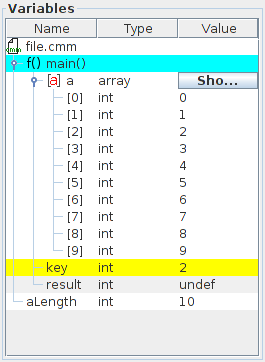
\includegraphics[width=1.0\textwidth]{./media/images/gui/var/treetable2.png}
		\caption{Darstellung der Variablen als Baum}\label{fig:deb-var-m2}
	\end{minipage}
\end{figure}

In den ersten Versionen der Benutzeroberfläche wurden die Variablen wie in Punkt 1 beschrieben dargestellt. Bereits während unseres Praktikums am Institut für Systemsoftware der JKU wurde die zweite Form der Variablendarstellung theoretisch entworfen. Die erste grundlegende Implementierung erfolgte noch während der Sommerferien.

In der ersten nummerierten Version, Alpha 1.0 (siehe \ref{sec:versions}), waren noch beide Darstellungsformen vorhanden und konnten vom Benutzer ausgewählt und gewechselt werden. Allerdings waren diese beiden Darstellungsformen sehr unterschiedlich implementiert, was Anfangs dazu führte, dass die Darstellung der Variablen als Baum nicht mehr als ein zusätzliches Feature ohne den vollen Funktionsumfang der Variablendarstellung als Call Stack war.

Für die Version Alpha 1.1 sollte ursprünglich das Variablendarstellungssystem so verändert werden, dass beide Anzeigemodi über ein gemeinsames Interface angesprochen werden können. Nach ausführlicher Besprechung und Evaluierung der unterschiedlichen Variablendarstellungen haben wir aber beschlossen, die Variablen nur als Baum darzustellen. Dadurch haben sich folgende Vorteile ergeben:
\begin{enumerate}
\item Die Implementierung einer neuen Funktion in der Variablenanzeige muss nur noch einmal erfolgen und nicht für jeden Anzeigemodus extra vorgenommen werden.
\item Daraus resultiert auch ein durchdachteres und einfacheres Bedienungskonzept der Benutzeroberfläche, da dieses nur an eine Variablendarstellung angepasst werden muss.
\item Davon profitiert zuletzt der Benutzer, der eine komplette und sauber implementierte Anzeige und Erklärung der Variablen während des Programmablaufes vorfindet.
\end{enumerate}

%	--------------------------------------------------------
% 	Darstellung in getrennten Tabellen
%	--------------------------------------------------------
\section{Darstellung der Variablen in getrennten Tabellen}

Diese Form der Variablendarstellung wurde erstmals im Dokument Ausführungsumgebung für C-- von Herrn Professor Blaschek beschrieben und nach dieser Vorlage implementiert\footnote{Ausführungsumgebung für C--, Günther Blaschek, V1.0, 2014-06-18}. Ein Vorteil dieser Darstellungsform war die Übersichtlichkeit und Einfachheit besonders beim Debuggen von einfachen Programmen. Leider verlor das Konzept an Übersichtlichkeit, wenn fortgeschrittene Programme mit komplexen Strukturen abgearbeitet wurden. Eine Tabelle konnte jeweils nur eine Ebene der Variablen, also beispielsweise den Inhalt einer Struktur oder die lokalen Variablen einer Funktion anzeigen.

%	--------------------------------------------------------
% 	Darstellung als Baum
%	--------------------------------------------------------
\section{Darstellung der Variablen als Baum}

\subsection{Darstellungsschema}

Die Darstellung der Variablen in Form einer Baumstruktur hat den Vorteil, dass alle Variablen in einem grafischen Element untergebracht sind und die Gültigkeitsbereiche der Variablen durch die hierarchische Baumstruktur sofort ersichtlich sind.

Die TreeTable besitzt drei Spalten: In der ersten befindet sich der Baum mit den Namen der Variablen. In der zweiten Spalte wird der Datentyp der Variable und in der dritten ihr Wert gezeigt.

Alle Elemente befinden sich in einem Ordner, der den Namen der Datei trägt. Dadurch wird symbolisiert, dass die Variablen ein Teil des Programms sind. Dem Programm selbst untergeordnet sind globale Variablen und Funktionen. Lokale Variablen sind Funktionen untergeordnet, Variablen in Strukturen sind der Struktur untergeordnet.
Zusätzlich werden folgende Elemente in der Tabelle farbig markiert:
\begin{itemize}
\item Funktionen sind hellblau hinterlegt. Sie sollen dadurch optisch von Datenstrukturen und Variablen unterscheidbar sein.
\item Die Variablen, die zuletzt geändert wurden, sind gelb hinterlegt. Grundsätzlich kann pro Schritt des Debuggers nur eine Variable geändert werden. Werden aber einige Schritte übersprungen, zum Beispiel mit dem Schlüsselwort \textbf{library}, so werden mehrere Variablen in einem Debuggerschritt geändert.
% TODO refer to library
\item Variablen, die noch nicht initialisiert wurden, sind grau hinterlegt.
% TODO refer to undef variables
\end{itemize}

\begin{figure}[htp]
\centering
\includegraphics[width=0.5\textwidth]{/home/fabian/Dokumente/C--/CMM/doc/de/media/images/gui/debugger/gui-treetable.png}
\caption{Beispiel für farbige Hervorhebung von Variablen}
\label{fig:deb-tt-example}
\end{figure}

%    ---------------------------------------------------------------------
%        Grundlegende Komponenten
%    ---------------------------------------------------------------------

\subsection{Grundlegende Komponenten}
Die Variablen werden in einer Tabelle mit Baumstruktur, deshalb auch \glqq{}TreeTable\grqq{} genannt, angezeigt. Die TreeTable ist eine Kombination aus einem JTree und einer JTable.
Im Folgenden werden diese Komponenten beschrieben und der Aufbau der TreeTable erläutert.

\subsubsection*{JTree - Baum}

\begin{wrapfigure}{r}{0.35\textwidth}
  	\begin{center}
    	\includegraphics[width=0.3\textwidth]{./media/images/gui/debugger/JTree-Example.png}
  	\end{center}
  	\caption{Beispiel für einen einfachen Baum}
	\label{fig:deb-tt-example-jtree}
\end{wrapfigure}

Ein JTree\footnote{http://www.codejava.net/java-se/swing/jtree-basic-tutorial-and-examples} ist Swing-Element, das Daten hierarchisch untereinander darstellt. Die Daten sind allerdings nicht im JTree selbst gespeichert, sondern in externen Objekten. Ein JTree kann entweder mit einem Datenmodell oder mit dem Hauptknoten eines Baumes initialisiert werden\footnote{http://docs.oracle.com/javase/tutorial/uiswing/components/tree.html}. Da die Daten eines JTree einen Baum abbildet, kann durch diese Struktur traversiert werden. Solche Operationen\footnote{http://www.java-tutorial.ch/core-java-tutorial/expande-or-collapse-all-nodes-in-a-jtree} werden beispielsweise benötigt, um alle Knoten eines Baumes zu öffnen (expand) oder zu schließen (collapse).

Wird ein JTree direkt mit einem Baum initialisiert, müssen die Knoten das Interface TreeNode implementieren\footnote{http://docs.oracle.com/javase/7/docs/api/javax/swing/tree/TreeNode.html}. Für einfache Aufgaben können Standardklassen, wie etwa DefaultMutableTreeNode\footnote{https://docs.oracle.com/javase/7/docs/api/javax/swing/tree/DefaultMutableTreeNode.html} verwendet werden.
Mehr Möglichkeiten bietet aber die explizite Verwendung eines Datenmodells. Ein Datenmodell regelt die Interaktion des JTree mit seinem Datenbaum und stellt Methoden zum Einfügen, Löschen und Ändern von Knoten sowie zum Auslesen des Pfades eines Knotens zur Verfügung.
Der JTree in der TreeTable von C Compact verwendet ein eigenes Datenmodell, TreeTableDataModel. Der Baum besteht aus Objekten der Klasse DataNode. Da ein eigenes Datenmodell verwendet wird, muss DataNode das Interface TreeNode nicht implementieren.

\subsubsection*{JTable - Tabelle}
Tabellen können in Swing mit dem Komponenten JTable\footnote{http://docs.oracle.com/javase/tutorial/uiswing/components/table.html} dargestellt werden. Wie auch bei der Klasse JTree werden die Daten nicht im Objekt von JTable gespeichert. Im einfachsten Fall kann eine Tabelle durch ein zweidimensionales Array initialisiert werden\footnote{http://www.java2s.com/Tutorial/Java/0240\_\_Swing/CreatingaJTable.htm}. In der Regel wird aber ein Datenmodell wie etwa DefaultTableModel\footnote{http://docs.oracle.com/javase/8/docs/api/javax/swing/table/DefaultTableModel.html} verwendet. Ein für eine Tabelle verwendbares Datenmodell ist ein Objekt einer Klasse, die das Interface TableModel\footnote{http://docs.oracle.com/javase/8/docs/api/javax/swing/table/TableModel.html} implementiert.

\begin{figure}[h]
\centering
\includegraphics[width=0.5\textwidth]{./media/images/gui/debugger/JTable-Example.png}
\caption{Beispiel für eine einfache Tabelle}
\label{fig:deb-tt-example-jtable}
\end{figure}

%    ---------------------------------------------------------------------
%        Allgemeine Implementierung
%    ---------------------------------------------------------------------

\subsection{Allgemeine Implementierung}
Die grundlegende Implementierung erfolgte anhand eines Blogeintrages\footnote{http://www.hameister.org/JavaSwingTreeTable.html}, mittlerweile wurde der Code allerdings stark an die Anforderungen der Benutzeroberfläche angepasst und erweitert.

Da die TreeTable auch zum Auswählen der Questpakete verwendet wird, wurden die meisten Komponenten der TreeTable so implementiert, dass sie auch für andere Anwendungen ohne Probleme weiterverwendet werden kann. Für jede Anwendung muss eine eigene Klasse für die Knoten des Baumes der TreeTable erstellt werden. Optional ist die Erweiterung durch eigene Renderer, der den Elementen der TreeTable unterschiedliche Symbole geben oder das Verwenden von Swing-Elementen in der Zelle einer Tabelle ermöglichen.

In Abbildung \ref{fig:deb-var-tt-class-raw} wird der Aufbau der TreeTable dargestellt. Swing - Komponenten sind Dunkelblau, von Java vorgegebene Klassen und Interfaces sind Hellblau dargestellt. Die meisten Klassen sind selbst implementiert und mit weiß gekennzeichnet. Orange gefärbte Klassen müssen für die jeweilige Anwendung selbst geschrieben bzw. angepasst werden.

Alle Klassen der TreeTable, die allgemein verwendet werden können, befinden sich im Package \textbf{at.jku.ssw.cmm.gui.treetable}.

\begin{figure}
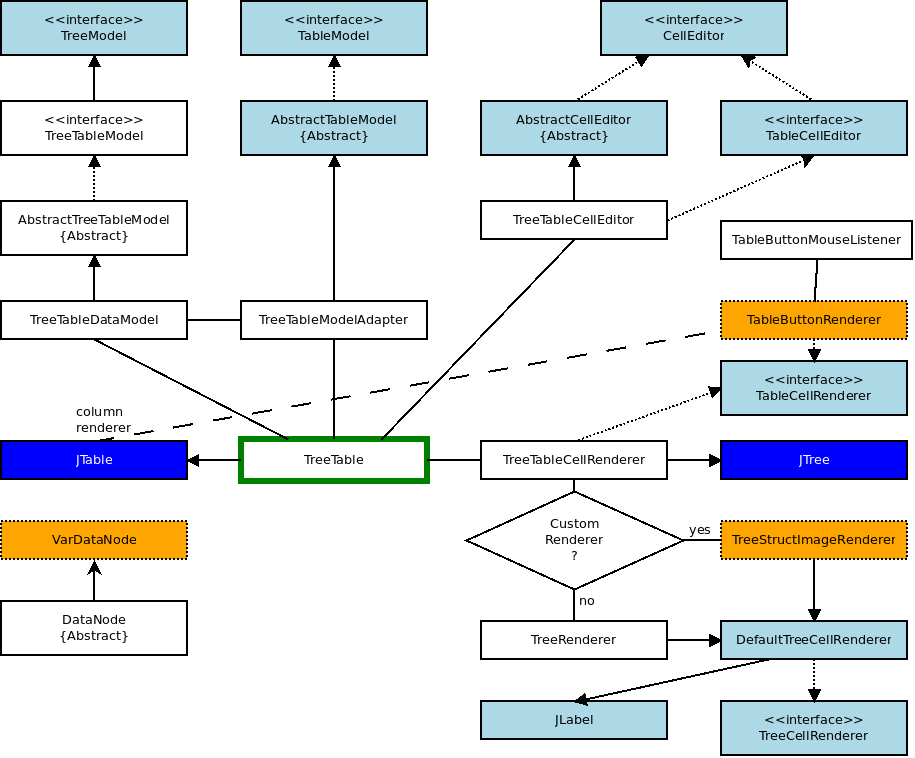
\includegraphics[width=\textwidth]{./media/images/gui/var/TreeTableClassesRaw.png}
\caption{Allgemeines Klassendiagramm der TreeTable}
\label{fig:deb-var-tt-class-raw}
\end{figure}

\subsubsection*{TreeTable}
Diese Klasse ist die Hauptklasse der TreeTable und, da sie von JTable erbt, eine Swing-Komponente. Von hier aus werden alle anderen Teile der TreeTable, wie etwa Datenmodelle und Renderer, verwendet.

Im Konstruktor werden einige Einstellungen an der Tablelle geändert. Diese Einstellungen können auch über die TreeTable selbst geändert werden (da sie von JTable erbt), allerdings sollte das vertauschen der Tabellenspalten deaktiviert bleiben (da sonst Probleme mit den Renderen des Baumes auftreten können).
\begin{lstlisting}[language=JAVA]
public TreeTable( TreeTableDataModel<TreeNode> treeTableModel ){
    super();
    this.setTreeModel(treeTableModel);
        
    //Do not allow column reordering
    getTableHeader().setReorderingAllowed(false);
        
    //Do not show the table grid
    setShowGrid(false);
        
    //No spacing
	setIntercellSpacing(new Dimension(0, 0));
}
\end{lstlisting}

Die Klasse \textbf{TreeTable} enthält zwei Methoden, die für die Implementierung besonders wichtig sind:
\begin{lstlisting}[language=JAVA]
public void setTreeModel( TreeTableDataModel<TreeNode> treeTableModel );
public void updateTreeModel();
\end{lstlisting}

Beide Methoden aktualisieren die angezeigten Daten in der TreeTable. Die Methode \textbf{setTreeModel(...)} muss verwendet werden, wenn ein neues Datenmodell angezeigt werden soll oder wenn sich die Struktur des Baumes verändert hat. Nach einfachen Wertänderungen in einem oder mehreren Knoten kann die Methode \textbf{updateTreeModel()} aufgerufen werden.

\subsubsection*{DataNode}
Ein Datenknoten (DataNode) ist ein Knoten des in der TreeTable abgebildeten Baumes. In diesen Knoten sind alle nötigen Informationen zu den angezeigten Variablen - auch jene, die nicht im Baum selbst sondern in der Tabelle angezeigt werden - gespeichert. Ein Knoten speichert immer alle Informationen einer ganzen Zeile.

DataNode ist eine abstrakte Basisklasse, die alle Daten enthält, die zur Verwendung in der TreeTable notwendig sind. Für die Anwendung muss eine eigene Node-Klasse implementiert werden, die von DataNode erbt.

\begin{lstlisting}[language=JAVA]
public abstract class DataNode {
	public abstract List<DataNode> getChildren();
	public abstract int getChildCount();
	public abstract Object getValueByColumn(int col);
	public abstract void addChild(DataNode n);
	@Override
	public abstract String toString();
	public void add(DataNode subNode) {
		// TODO Auto-generated method stub
		
	}
}
\end{lstlisting}

DataNode selbst enthält keine Datenstruktur, die Referenzen zu untergeordneten Knoten im Baum speichert. Die Methode \textbf{getChildren()} muss aber eine Liste mit Referenzen zurückgeben. Diese Liste sollte in einer von DataNode abgeleiteten Klasse implementiert werden.

Die \textbf{toString}-Methode muss überschrieben werden, da diese beim Rendern des Baumes verwendet wird. \textbf{toString()} sollte den Anzeigenamen des Datenknoten (der Name, der im Baum der TreeTable angezeigt wird) übergeben. Die Implementierung der Methode \textbf{add()} ist empfehlenswert (da der Baum irgendwie aufgebaut werden muss) aber nicht erforderlich.
%TODO read first two sentences

\subsubsection*{TreeModel}
TreeModel ist ein Interface für alle Datenmodelle eines JTree.

\subsubsection*{TreeTableModel}
Dieses Interface erweitert das Interface \textbf{TreeModel} so, dass es mit einer TreeTable kompatibel wird. TreeTableModel definiert zusätzliche Methoden, die für das Datenmodell einer Tabelle benötigt werden, beispielsweise \textbf{getColumnName()}.

\subsubsection*{AbstractTreeTableModel}
Diese abstrakte Basisklasse implementiert einige konkrete Methoden für die Verwendung als Datenmodell eines JTree. In Objekten dieser Klasse wird der Basisknoten (root) des Baumes gespeichert. Außerdem regelt AbstractTreeModel den Ablauf von Änderungsevents in der Datenstruktur des Baumes.

\subsubsection*{TreeTableDataModel}
%TODO read this subsubsection
TreeTableDataModel erbt von AbstractTreeTableModel und ist ein vollständiges Tabellen-Datenmodell. Außerdem wird in dieser Klasse das konkrete Aussehen der TreeTable festgelegt, indem die Tabellenspalten definiert werden.
\begin{lstlisting}[language=JAVA]
public class TreeTableDataModel<TreeNode extends DataNode> extends AbstractTreeTableModel<TreeNode> {

	public TreeTableDataModel(TreeNode rootNode, String[] columnNames, Class<?>[] columnTypes, int currFunc) {
		super(rootNode);
		...
    }
    ...
}
\end{lstlisting}

Um die TreeTable zu initialisieren, muss ein Objekt dieser Klasse erstellt werden. Dabei müssen der Hauptknoten des Datenbaumes (ein Objekt, das von \textbf{DataNode} erbt) und Namen und Datentypen der jeweiligen Tabellenspalten angegeben werden.
\begin{lstlisting}[language=JAVA]
String[] columnNames = { _("Name"), _("Type"), _("Value") };
Class<?>[] columnTypes = { TreeTableModel.class, String.class, Object.class };

treeTableModel = new TreeTableDataModel<VarDataNode>(InitTreeTableData.createDataStructure(fileName), columnNames, columnTypes);
\end{lstlisting}

\subsubsection*{TableModel}
Dieses Interface bildet die Grundlage für alle Datenmodelle einer JTable\footnote{http://docs.oracle.com/javase/7/docs/api/javax/swing/table/TableModel.html}.

\subsubsection*{AbstractTableModel}
In dieser abstrakten Basisklasse sind bereits die meisten Methoden des Interface TreeModel implementiert\footnote{http://docs.oracle.com/javase/7/docs/api/javax/swing/table/AbstractTableModel.html}. Alle dazu noch benötigten Methoden werden in der Klasse \textbf{TreeTableModelAdapter} definiert.

\subsubsection*{TreeTableModelAdapter}
TreeTableModelAdapter bildet die Verbindung zwischen dem Datenmodell der Tabelle und dem des Baumes. Diese Klasse erbt von AbstractTreeTableModel und enthält eine Referenz auf TreeTableDataModel. Viele Methoden, wie etwa \textbf{getColumnName(...)} oder \textbf{getValueAt(...)} sind in TreeTableDataModel implementiert, da sich in dieser Klasse auch das eigentliche Datenmodell der TreeTable befindet, und werden in TreeTableModelAdapter übernommen. Beispielsweise greifen die folgenden Methoden auf die Implementierung in TreeTableDataModel zurück:
\begin{lstlisting}[language=JAVA]
public Object getValueAt(int row, int column) {
   return treeTableModel.getValueAt(nodeForRow(row), column);
}

public boolean isCellEditable(int row, int column) {
   return treeTableModel.isCellEditable(nodeForRow(row), column);
}
\end{lstlisting}

\subsubsection*{CellEditor}

Der Inhalt einer Tabelle oder eines Baumes kann, je nach Konfiguration, von unterschiedlichen Komponenten geändert werden. Zum Beispiel kann ein String in einer Tabelle mit einem JTextField und ein boolean-Wert mit einer JCheckBox geändert werden.

Damit Informationen über Editorobjekte nicht in JTree, JTable und ähnlichen Komponenten einzeln implementiert werden müssen, gibt es das Interface \textbf{CellEditor}. Dieses bildet eine Schicht zwischen dem Editor (zum Beispiel einem JTextField) und dem übergeordneten Komponenten(zum Beispiel einer JTable).

Die einfachse Implementierung von CellEditor ist der DefaultCellEditor\footnote{https://docs.oracle.com/javase/7/docs/api/javax/swing/DefaultCellEditor.html}. Dieser unterstützt die Eingabe von Daten in die Tabelle mithilfe eines Textfeldes, einer Checkbox oder einer Combobox.

\subsubsection*{AbstractCellEditor}
AbstractCellEditor ist eine abstrakte Basisklasse für alle Arten eines CellEditor in Swing\footnote{https://docs.oracle.com/javase/7/docs/api/javax/swing/AbstractCellEditor.html}. Einige grundlegende Methoden sind bereits implementiert.

\subsubsection*{TableCellEditor}
Dieses Interface\footnote{http://docs.oracle.com/javase/7/docs/api/javax/swing/table/TableCellEditor.html} definiert die Methode \textbf{getTableCellEditorComponent(...)}. Diese Methode sollte den Editor (also den Swing-Komponenten, der verwendet wird, um den Inhalt der betroffenen Zelle zu modifizieren) zurückgeben.

\subsubsection*{TreeTableCellEditor}
Daten in der TreeTable sollen vom Benutzer zwar nicht verändert werden können, wenn das Editieren der Tabelle mit der Methode \textbf{setEditable()} aber deaktiviert wird, werden auch Events (wie etwa Mausklicks) nicht mehr registriert. TreeTableCellEditor gibt also Events in der Tabelle bei Bedarf an den JTree weiter und verbietet Events in Zellen, die nur Text enthalten.
\begin{lstlisting}[language=JAVA]
public boolean isCellEditable(EventObject e) {
	if (e instanceof MouseEvent) {
     	MouseEvent me = (MouseEvent) e;
    	MouseEvent newME = new MouseEvent(tree, me.getID(), me.getWhen(), me.getModifiers(), me.getX() - table.getCellRect(0, 0, true).x, me.getY(), 2, me.isPopupTrigger());
    	tree.dispatchEvent(newME);
  	}
  	return false;
}
\end{lstlisting}

Außerdem wird die Methode \textbf{getTableCellEditorComponent(...)} aus dem Interface \textbf{TableCellEditor} implementiert. Diese Methode gibt den JTree zurück, wenn dessen Tabellenspalte angeklickt wurde. Ansonsten wird die Tabelle zurückgegeben.
\begin{lstlisting}[language=JAVA]
public Component getTableCellEditorComponent(JTable table, Object value, boolean isSelected, int r, int c) {
    if( c == 0 )
        return this.tree;
    else
        return this.table;
}
\end{lstlisting}

\subsubsection*{TableCellRenderer}
In diesem Interface sind alle Methoden definiert, die zum Rendern von Zellen einer JTable benötigt werden\footnote{https://docs.oracle.com/javase/7/docs/api/javax/swing/table/TableCellRenderer.html}.

\subsubsection*{TreeTableButtonMouseListener}
Diese Klasse implementiert das Interface \textbf{MouseListener} und ist Event Listener der gesamten TreeTable. Dieser Listener muss allerdings manuell zur TreeTable hinzugefügt werden.
\begin{lstlisting}[language=JAVA]
treeTable.addMouseListener(new TableButtonMouseListener(main, treeTable));
\end{lstlisting}

Der Listener \textbf{TreeTableButtonMouseListener} sorgt dafür dass, falls ein Button in der Tabelle angeklickt wird, der entstandene Event an den Button weitergeleitet wird, sodass der Button seinen eigenen EventListener ausführen kann.
\begin{lstlisting}[language=JAVA]
public void mouseClicked(MouseEvent e) {
	// Leitet den Event an den angeklickten Button weiter
	forwardEventToButton(e, this.treeTable.getTable().rowAtPoint(e.getPoint()), this.treeTable.getTable().columnAtPoint(e.getPoint()));
}
\end{lstlisting}

\subsubsection*{TreeTableCellRenderer}
Diese Klasse erbt von JTree und wird verwendet, um einen Baum in die erste Spalte der Treetable zu rendern. Außerdem ist diese Klasse dafür verantwortlich, dass die Zeilen der Tabelle und des Baumes die selbe Höhe haben und dass die Zellen die richtige Farbe erhalten.

An den JTree selbst kann außerdem noch ein eigens erstellter Renderer übergeben werden, um beispielsweise eigene Symbole für jeden Knoten im Baum anzuzeigen. Dieser Renderer muss das Interface \textbf{DefaultTreeCellRenderer} implementieren. Ist ein solcher Renderer nicht vorhanden, wird die standardmäßig \textbf{TreeRenderer} verwendet.

\subsubsection*{JLabel}
Ein JLabel\footnote{http://docs.oracle.com/javase/7/docs/api/javax/swing/JLabel.html} ist ein einfaches Swing-Element, das einen Text und/oder ein Bild anzeigen kann. Für den Text in der Zelle einer Tabelle oder dem Knoten eines Baumes werden meistens JLabels verwendet (außer die Zelle soll editierbar sein; dann wird ein JTextField\footnote{http://docs.oracle.com/javase/7/docs/api/javax/swing/JTextField.html} verwendet). JLabels reagieren nicht auf Events, wie etwa Mausklicks.

\subsubsection*{TreeCellRenderer}
Diese Interface definiert Basismethoden für ein Objekt, das den Knoten eines JTree rendern kann\footnote{http://docs.oracle.com/javase/7/docs/api/javax/swing/tree/TreeCellRenderer.html}.

\subsubsection*{DefaultTreeCellRenderer}
Diese Klasse enthält Implementierungen zum Rendern von Knoten eines JTree\footnote{http://docs.oracle.com/javase/7/docs/api/javax/swing/tree/DefaultTreeCellRenderer.html}.

\subsubsection*{TreeRenderer}
Dieser Renderer wird für den JTree der TreeTable verwendet, wenn kein anderer Renderer vorhanden ist. Die Klasse TreeRenderer entfernt alle Hintergrundfarben des JTree, damit die Farbmarkierungen in den Zeilen der Tabelle auch hinter dem Text der JTree-Knoten sichtbar sind. Das muss auch bei allen eigenen JTree-Renderern für die TreeTable berücksichtigt werden. In einen eigenen Renderer müssen folgende Methoden implementiert werden:
\begin{lstlisting}[language=JAVA]
@Override
public Color getBackgroundNonSelectionColor() {
    return null;
}

@Override
public Color getBackgroundSelectionColor() {
    return null;
}

@Override
public Color getBackground() {
    return null;
}
\end{lstlisting}

Ohne diese Methoden zeichnet der JTree die Texte (JLabel) seiner Knoten nicht mit transparentem Hintergrund (Vergleiche Abbildung \ref{fig:deb-tt-render-no} und \ref{fig:deb-tt-render-yes}).

\begin{figure}[h!]
\centering
	\begin{minipage}{0.45\textwidth}
		\centering
		\includegraphics[width=1.0\textwidth]{./media/images/gui/var/tt-norender.png}
		\caption{TreeTable ohne Renderer für den JTree}\label{fig:deb-tt-render-no}
	\end{minipage}\hfill
	\begin{minipage}{0.48\textwidth}
		\centering
		\includegraphics[width=1.0\textwidth]{./media/images/gui/var/tt-render.png}
		\caption{TreeTable mit Renderer für den JTree}\label{fig:deb-tt-render-yes}
	\end{minipage}
\end{figure}

%    ---------------------------------------------------------------------
%        Spezielle Implementierung
%    ---------------------------------------------------------------------
\subsection{Implementierung für den Debugger}
\label{sec:deb-var-special}
Hier werden die Erweiterungen an der TreeTable beschrieben, die für die Anwendung im Debugger nötig waren. Für andere Anwendungen kann die TreeTable ähnlich erweitert und implementiert werden.

\subsubsection*{TreeTableView}
TreeTableView ist eine Wrapperklasse für TreeTable. Sie übernimmt alle wichtigen Funktionen zur Kommunikation mit dem Variablenbaum und bildet so eine Schicht zwischen dem Debugger und der TreeTable. Auf diese Weise wird der Code übersichtlicher und ist besser strukturiert.
TreeTableView hat folgende Methoden:
\begin{itemize}
\item \textbf{init} Initialisiert die TreeTable mit einem Standard-Datenmodell. Dieses besteht nur aus einem Hauptknoten (root), der den Namen der aktuellen Datei trägt; es werden keine Variablen angezeigt. Das Standard-Datenmodell wird immer dann angezeigt, wenn der Debugger nicht aktiv ist, also wenn der Benutzer den Sourcecode editiert.
\item \textbf{standby} Löscht das aktuelle Datenmodell und übergibt ein Standard-Datenmodell an die TreeTable, sodass wie zu Beginn nur der aktuelle Dateiname angezeigt wird. Diese Methode wird immer aufgerufen, wenn der Debugger beendet wird.
\item \textbf{update} Aktualisiert das Datenmodell der TreeTable im Debugmodus und zeigt die Variablen im Speicher des Interpreters an.
\item \textbf{highlightVariable} Mit dieser Methode wird die Adresse einer zuletzt geänderten Variable an die TreeTable übergeben. Diese Variable wird in der Tabelle markiert. Es ist möglich, diese Funktion mehrmals aufzurufen und so mehrere Variablen zu markieren. Wenn das Datenmodell mit \textbf{update} aktualisiert wird, verfallen alle Markierungen.
\item \textbf{updateFontSize} Bei Aufruf dieser Methode wird die Schriftgröße der Tabelle geändert und die gesamte TreeTable neu gezeichnet. Diese Methode wird aufgerufen, wenn die Einstellungen der Benutzeroberfläche geändert wurden.
\end{itemize}

\subsubsection*{VarDataNode}
Die Klasse VarDataNode erweitert die abstrakte Klasse DataNode und kann deshalb für die Datenstruktur der TreeTable verwendet werden. Ein VarDataNode bildet einen Knoten im Baum bzw. eine Zeile in der TreeTable.

Folgende Daten werden in einem Knoten gespeichert:
\begin{lstlisting}[language=JAVA]
// Informationen, die in der Tabelle angezeigt werden
private final String name;
private Object type;
private Object value;

// Zusätzliche Informationen
private int address;
\end{lstlisting}
Die Felder für Datentyp und Wert haben den Typ Object, da sich in der Tabelle an der Stelle eines Wertes auch ein JButton befinden kann (zum Beispiel bei Strings).

Zusätzlich wird die Adresse der Variable gespeichert. Die Adresse dient der eindeutigen Identifikation der Variable, zum Beispiel beim Traversieren durch den Variablenbaum.
%TODO mention treeUtils

\subsubsection*{TableButtonRenderer}
Diese Klasse sorgt dafür, dass die Zellen der Tabelle die vorgesehene Hintergrundfarbe erhalten und dass AWT- und Swing-Elemente in der Tabelle gerendert dargestellt werden. Um Elemente der grafischen Benutzeroberfläche in einer Tabelle zu rendern, muss die Methode \textbf{getTableCellRendererComponent(...)} für die jeweilige Zelle das beinhaltete Element zurückgeben.
\begin{lstlisting}[language=JAVA]
public Component getTableCellRendererComponent(JTable table, Object value, boolean isSelected, boolean hasFocus, int row, int column) {
	Component c = (Component)defaultRenderer.getTableCellRendererComponent(table, value, isSelected, hasFocus, row, column);
	
	// AWT- oder Swing-Komponente verwenden
	if(value instanceof Component)
		return (Component)value;
	
	// Weitere Anpassungen (Hintergrundfarben der Zellen)
	else if( ... )
		...
		//Hintergrundfarbe einer Zelle ändern
		c.setBackground(new Color(0, 159, 153));
		...
	
	return c;
}
\end{lstlisting}

\subsubsection*{TreeStructImageRenderer}
Dieser Renderer wird anstelle des Standardrenderers \textbf{TreeRenderer} der TreeTable verwendet. Wie im TreeRenderer sind auch hier Methoden implementiert, um die Hintergrundfarben der Knoten des JTree zu entfernen, sodass die jeweilige Hintergrundfarbe der Tabellenzelle sichtbar ist. Außerdem ist eine weitere Methode implementiert, die den Knoten des Baumes je nach Datentyp ein anderes Icon gibt.

Zum Ändern des Icons eines Knoten muss im Renderer folgende Methode implementiert werden:
\begin{lstlisting}[language=JAVA]
public JComponent getTreeCellRendererComponent(JTree tree, Object value, boolean sel, boolean exp, boolean leaf, int row, boolean hasFocus) {

	ImageIcon icon = new ImageIcon("images/icon.png");

	setOpenIcon(icon);
	setClosedIcon(icon);
	setLeafIcon(icon);
	
	super.getTreeCellRendererComponent(tree, value, sel, exp, leaf, row, hasFocus);
		
	return this;
}
\end{lstlisting}

Für verschiedenen Arten von Einträgen in der Variablentabelle werden unterschiedliche Bilder verwendet:
\def\arraystretch{1.4}
\begin{table}[h!]
\center
\begin{tabular}{|cl|}
\hline 
Bild & Art des Eintrages \\ 
\hline
\includegraphics[scale=1.0]{./media/images/gui/var/icons/cmm.png} & Hauptknoten: Die CMM-Datei selbst \\
\includegraphics[scale=1.0]{./media/images/gui/var/icons/func.png} & Funktionen \\
\includegraphics[scale=1.0]{./media/images/gui/var/icons/struct.png} & Strukturen \\ 
\includegraphics[scale=1.0]{./media/images/gui/var/icons/array.png} & Arrays (nur der übergeordnete Knoten, nicht die Indizes) \\ 
- & Einfache Datentypen haben kein Bild\\
\hline 
\end{tabular}
\caption{Icons für unterschiedliche Strukturen und Einträge in der Variablentabelle}
\end{table}

\section{Auslesen der Variablen}

%TODO ref speicher, call stack, Symboltabelle
Die Variablen des laufenden Programms werden nach jedem Schritt des Interpreters neu ausgelesen. Dabei wird zuerst der \textbf{Call Stack} abgearbeitet. Für jede Funktion wird durch die \textbf{Symboltabelle} iteriert. Dabei werden Knoten für die Variablentabelle (siehe Kapitel \ref{sec:deb-var-special}, VarDataNode) angelegt. Die Werte der Variablen werden aus dem \textbf{Speicher} ausgelesen.
%TODO hier noch codebeispiele?

Das Datenmodell für die TreeTable wird von Methoden der Klasse \textbf{InitTreeTableDate} im Package \textbf{at.jku.ssw.cmm.debugger} erstellt. Um ein neues Datenmodell zu erstellen, muss die Methode \textbf{readSymbolTable} aufgerufen werden.
\begin{lstlisting}[language=JAVA]
public static TreeTableDataModel<VarDataNode> readSymbolTable( CMMwrapper compiler, GUImain main, String fileName, String[] columnNames, Class<?>[] columnTypes );
\end{lstlisting}

Das bestehende Datenmodell kann mit der Methode \textbf{updateTreeTable} aktualisiert werden.
\begin{lstlisting}[language=JAVA]
public static void updateTreeTable( TreeTableDataModel<VarDataNode> model, VarDataNode node, CMMwrapper compiler, GUImain main, String fileName );
\end{lstlisting}



%   Popups
%!TEX root = "../../../DA_GUI.tex"

%	--------------------------------------------------------
% 	Debugger: Popups
%	--------------------------------------------------------


\section{Popups}
\label{sec:deb-popup}
Im Debugger von C Compact gibt es mehrere Anwendungsfälle für Popup-Fenster. Popups werden verwendet, um weitere Informationen zu einem Array oder einem String in der Variablentabelle zu liefern und um Rückgabewerte von Funktionen zu visualisieren (dies ist allerdings optional, siehe auch \ref{sec:win-set}). Dabei handelt es sich im Prinzip um kleine Anzeigeflächen, die ein Swing-Element enthält (siehe Abbildung \ref{fig:popup-example}). Ein Popup wird ausgeblendet, sobald auf eine beliebige Fläche in einem Fenster von C Compact --- außerhalb des Popups --- geklickt wird.

\begin{figure}[htp]
\centering
\includegraphics[width=0.4\textwidth]{./media/images/gui/popup/popup-example.png}
\caption{Ein Popup zeigt den Rückgabewert einer Funktion.}
\label{fig:popup-example}
\end{figure}

\subsection{Initialisierung eines Popups}
Alle für das Popup relevanten Klassen befinden sich im Package \textbf{at.jku.ssw.cmm.gui.popup}. Die Popup-Funktionen selbst befinden sich in der Klasse \textbf{ImagePopup}. Zum Initialisieren werden aber die statischen Methoden in der Klasse \textbf{ComponentPopup} verwendet; diese Methoden übernehmen auch umständliche Positionsberechnungen für das Popup. Die Methode \textbf{createPopUp(...)} kann auch ohne das Parameter \glqq{}weight\grqq{} verwendet werden.
\begin{lstlisting}[language=JAVA]
public static void createPopUp( GUImain main, JComponent component, int x, int y, int w, int h, int orientation, double weight );
\end{lstlisting}

\begin{table}[h!]
\begin{tabular}{|ll|l|}
\hline 
GUImain & main  & Referenz auf das Hauptfenster, siehe \ref{sec:gui-main-impl} \\
\hline
JComponent & component & Das Swing-Element, das angezeigt werden soll \\
\hline
int & x & \multirow{2}{8cm}{Die Position, auf die das Popup zeigen soll} \\
int & y & \\
\hline 
int & w & \multirow{2}{8cm}{Höhe und Breite des Popups (Bezogen auf den äußeren Rand, \textbf{component} wird mit 5px Inset platziert)} \\
int & h & \\
\hline
int & orientation & Ausrichtung des Popups (siehe Unten) \\
\hline
double & weight [optional] & Position des Zeigers, Wert zwischen 0 und 1, Standard: 0.5\\
\hline
\end{tabular}
\caption{Parameter der Methode \textbf{createPopup(...)}}
\end{table}

\begin{figure}[h!]
\centering
\includegraphics[width=0.4\textwidth]{./media/images/gui/popup/popup-pos.png}
\caption{Positionierung eines Popups}\label{fig:deb-popup-pos}
\end{figure}

Der Parameter \textbf{orientation} legt fest, in welche Richtung das Popup zeigt. Das Popup hat immer einen Zeiger, der auf die mit \textbf{x} und \textbf{y} angegebene Position zeigt (siehe Abbildung \ref{fig:deb-popup-pos}). Für den Parameter \textbf{orientation} stehen vier Möglichkeiten zur Verfügung. Die Konstanten sind in der Klasse \textbf{ImagePopup} definiert:
\begin{itemize}
\item \textbf{NORTH:} Zeiger befindet sich am oberen Rand
\item \textbf{SOUTH:} Zeiger befindet sich am unteren Rand
\item \textbf{WEST:} Zeiger befindet sich am linken Rand
\item \textbf{EAST:} Zeiger befindet sich am rechten Rand
\end{itemize}

Mit dem Parameter \textbf{weight} kann die Position des Zeigers am Popup bestimmt werden. Der Wert 0 bedeutet, dass der Zeiger --- je nach Ausrichtung --- ganz links oder ganz oben ist. Wird dieser Parameter nicht angegeben, hat \textbf{weight} den Wert \textbf{0.5}.

\subsection{Implementierung}
Die Methoden zum Erstellen und Zeichnen des Popups befinden sich in der Klasse \textbf{ImagePopup}. Diese muss mit weniger praktischen Parametern initialisiert werden: mit x und y ist beispielsweise die linke obere Ecke des Popups anzugeben. Deshalb werden zum Initialisieren die statischen Methoden in der Klasse ComponentPopup verwendet. Diese rechnen die angegebenen Parameter auf die Popup-Positionen um.

\subsubsection*{Das Popup in das Hauptfenster zeichnen}
In Swing besteht jedes Fenster aus mehreren Schichten\footnote{https://docs.oracle.com/javase/tutorial/uiswing/components/rootpane.html}, die unterschiedliche Aufgaben übernehmen. Die oberste Schicht ist das sogenannte \textbf{GlassPane}. Dieses Panel ist standardmäßig deaktiviert. Wird es aktiviert, kann es verwendet werden, um über die Komponenten des Hauptfensters zu zeichnen und Events des Fensters abzufangen\footnote{https://docs.oracle.com/javase/tutorial/uiswing/components/rootpane.html\#glasspane}.

Die Klasse \textbf{ImagePopup(...)} erbt von \textbf{JPanel} und ist daher eine einfache Swing-Komponente. 

Mit der Methode \textbf{invokePopup(...)} wird eine beliebige Komponente zum GlassPane hinzugefügt und dort gezeichnet. Diese Methode befindet sich in der Klasse \textbf{GUImain} (siehe Kapitel \ref{sec:gui-main}), die das Hauptfenster von C Compact verwaltet.
\begin{lstlisting}[language=JAVA]
public void invokePopup(JPanel popup, int x, int y, int width, int height) {

	// Popup wird zum GlassPane hinzugefügt
	((JPanel) this.jFrame.getGlassPane()).add(popup);
	
	// Listener zum Schließen des Popuos wird initialisiert
	((JPanel) this.jFrame.getGlassPane()).addMouseListener(
		new PopupCloseListener(this.jFrame, ((JPanel) this.jFrame.getGlassPane()), popup, x, y, width, height));
		
	// GlassPane neu zeichnen
	((JPanel) this.jFrame.getGlassPane()).validate();
	((JPanel) this.jFrame.getGlassPane()).repaint();
}
\end{lstlisting}

In der Klasse \textbf{ImagePopup} wird die Methode \textbf{paintComponent}\footnote{http://www.oracle.com/technetwork/java/painting-140037.html\#callbacks} überschrieben. Dies ist eine der drei Methoden, die aufgerufen werden, wenn die Benutzeroberfläche neu gerendert werden muss. In gewisser Weise entspricht das der \textbf{paint}-Methode in ATW, allerdings spaltet Swing das Rendern auf drei unterschiedliche Methoden auf: \textbf{paintComponent} zeichnet das Element selbst, \textbf{paintBorder} zeichnet den Rand des Komponenten und \textbf{paintChildren} rendert die Komponenten innerhalb des zu zeichnenden Elementes. Durch diese Aufteilung können Manipulationen am Rendering eines Komponenten gezielter vorgenommen werden.

\begin{lstlisting}[language=JAVA]
@Override
public void paintComponent(Graphics g) {
        
    // Grenzen des Komponenten werden gesetzt
    switch( this.orientation ) {
    case NORTH:
    	g.setClip(g.getClipBounds().x, g.getClipBounds().y-10, g.getClipBounds().width, g.getClipBounds().height+10);
    	break;
    case SOUTH:
    	g.setClip(g.getClipBounds().x, g.getClipBounds().y, g.getClipBounds().width+10, g.getClipBounds().height+10);
    	break;
    case WEST:
    	g.setClip(g.getClipBounds().x-10, g.getClipBounds().y, g.getClipBounds().width+10, g.getClipBounds().height);
    	break;
    case EAST:
    	g.setClip(g.getClipBounds().x, g.getClipBounds().y, g.getClipBounds().width+10, g.getClipBounds().height);
    	break;
    }
    // Die Rendering-Methoden der Basisklasse werden aufgerufen
    super.paintComponent(g);
    super.paintBorder(g);
    	
    // Der Zeiger wird gezeichnet
    switch( this.orientation ) {
    case NORTH:
    	g.drawImage(image, centerX-10, centerY, image.getWidth(null), image.getHeight(null), this);
    	break;
    case SOUTH:
    	g.drawImage(image, centerX-10, centerY-15, image.getWidth(null), image.getHeight(null), this);
    	break;
    case WEST:
    	g.drawImage(image, centerX, centerY-10, image.getWidth(null), image.getHeight(null), this);
    	break;
    case EAST:
    	g.drawImage(image, centerX-15, centerY-10, image.getWidth(null), image.getHeight(null), this);
    	break;
    }
}
\end{lstlisting}

Mit der Methode \textbf{setClip} wird der Zeichenbereich des Popups so erweitert, dass der Zeiger gezeichnet werden kann, obwohl er außerhalb des JPanels liegt.

\subsubsection*{Popups mit Tabellen}
Um den Inhalt eines Arrays anschaulicher darzustellen, kann das Array in einem Popup geöffnet werden. Es wird dann als Tabelle dargestellt.

\begin{figure}[h!]
\centering
	\begin{minipage}{0.45\textwidth}
		\centering
		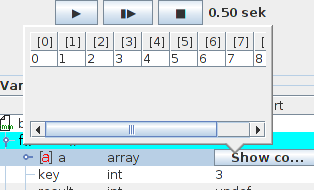
\includegraphics[width=1.0\textwidth]{./media/images/gui/popup/array1dim.png}
		\caption{Ein eindimensionales Array wird in einem Popup dargestellt}
		\label{fig:gui-popup-a1}
	\end{minipage}\hfill
	\begin{minipage}{0.46\textwidth}
		\centering
		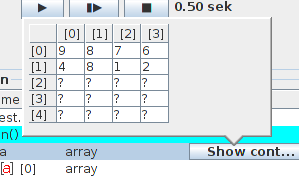
\includegraphics[width=1.0\textwidth]{./media/images/gui/popup/array2dim.png}
		\caption{Ein zweidimensionales Array wird in einem Popup dargestellt}
		\label{fig:gui-popup-a2}
	\end{minipage}
\end{figure}

Tabellen können grundsätzlich wie alle anderen Komponenten in einem Popup dargestellt werden. Für die Implementierung im Debugger (Abbildung \ref{fig:gui-popup-a1} und Abbildung \ref{fig:gui-popup-a2}) wurden allerdings ein eigenes Datenmodell und ein eigener Renderer erstellt. \textbf{TablePopupModel} ist ein Datenmodell, das den Inhalt eines Arrays korrekt darstellen kann. Für zweidimensionale Arrays wird die erste Tabellenspalte mit \textbf{TablePopupRenderer} gezeichnet, sodass sie wie die Kopfspalte der Tabelle aussieht (Abbildung \ref{fig:gui-popup-a2}).



%   Fehlerbeschreibungen
%!TEX root = "../../../DA_GUI.tex"

%	--------------------------------------------------------
% 	Debugger: Fehleranzeige
%	--------------------------------------------------------

\section{Anzeige von Programmfehlern}
\label{sec:deb-error}
Im Quelltext des Benutzers können unterschiedliche Arten von Fehlern enthalten sein, die dazu führen, dass der Debugger entweder nicht gestartet werden kann (Probleme im Präprozessor oder beim Compilieren) oder dass der Debugger beendet wird (Laufzeitfehler). Allerdings wissen gerade unerfahrene Programmierer oft nicht, wodurch das Problem verursacht wurde und haben deshalb auch Schwierigkeiten, den Fehler zu finden und zu beheben.

Bei Versuchen mit Schülern wurde erneut besonders deutlich, dass die Fehlermeldungen des Compilers für Programmieranfänger keine große Hilfe sind (siehe Kapitel \ref{sec:sci-trial-gui}).

Beim Debuggen aufgetretene Fehler --- diese sollten nicht mit internen Fehlern verwechselt werden (siehe Kapitel \ref{sec:gui-int-error}) --- werden in C Compact im Sourcecode rot markiert, außerdem zeigt das Zustandspanel des Debuggers Fehlername und die Zeilennummer an (siehe Kapitel \ref{sec:gui-main-left-zust}). Im rechten Teil der Benutzeroberfläche wird eine detaillierte Beschreibung des Fehlers mit möglichen Ursachen und Hinweisen zur Fehlersuche gezeigt (siehe Kapitel \ref{sec:gui-main-right-error}). Abbildung \ref{fig:deb-error-gui} zeigt das Hauptfenster von C Compact, wenn ein Fehler aufgetreten ist.
%TODO read last words of this paragraph again

\begin{figure}[h!]
\centering
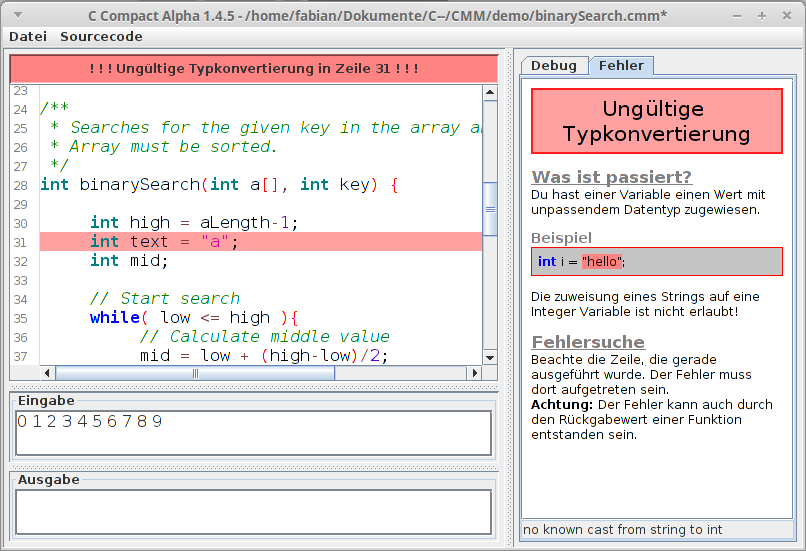
\includegraphics[width=0.8\textwidth]{./media/images/gui/debugger/gui-error-2.png}
\caption{Ein Fehler im Quelltext wird angezeigt}\label{fig:deb-error-gui}
\end{figure}

Diese Fehlerbeschreibungen werden im Ordner \textbf{error} in einem Unterordner mit dem jeweiligen Sprachkennzeichen --- zum Beispiel \textbf{de} für Deutsch --- als HTML-Dokumente gespeichert. Im Ordner \textbf{error} befinden sich außerdem die Dateien \textbf{table.xml} und \textbf{style.css}. In der Datei \textbf{table.xml} werden Fehlermeldungen einzelner Komponenten von C Compact mit der zugehörigen Beschreibungsdatei verknüpft. Dabei sind auch reguläre Ausdrücke erlaubt. Das Codebeispiel unten beinhaltet zuerst eine Zuweisung für mehrere ähnliche Fehlermeldungen und dann die Zuweisung eines bestimmten Fehlers zu einem Dokument. Der Pfad des Beschreibungsdokumentes wird unabhängig vom jeweiligen Sprachordner angegeben, sodass die Fehlermeldung in der eingestellten Sprache geladen werden kann.
\begin{lstlisting}[language=XML]
<error id="no known cast from ([\w./\s]+)">
	<file>cast.html</file>
</error>
<error id="variable assigment is not allowed in struct">
	<file>compiler/variable_decl/struct_var_assign.html</file>
</error>
\end{lstlisting}

Für unbekannte Fehlermeldungen ist die Datei \textbf{default.html} im jeweiligen Sprachordner vorhanden.
%TODO alle englischen Fehlerdokumente vorhanden?

Die Datei \textbf{style.css} enthält die Formatierungsinformationen für die Fehlerdokumente




\else
	\chapter{Benutzeroberfläche}
	\section{Launcher}
Der Launcher ist ein eigenes Fenster, welches vor dem Öffnen der Benutzeroberfläche angezeigt wird. Hier hat der Benutzer die Möglichkeit, eigene Profile zu erstellen, die Sprache zu ändern und sein Benutzerprofil zu starten. Auch werden hier die zuletzt geöffneten Profile dargestellt.

\begin{figure}[h] 
  \centering
     \includegraphics[width=0.9\textwidth]{./media/images/gui/launcher/launcher_main.png}
  \caption{Launcher GUI}
  \label{fig:launcher_GUI}
\end{figure}

%TODO Verwei auf Anhang
Grundsätzlich ist der Launcher ein JFrame\footnote{\url{http://www.java-tutorial.org/jframe.html}}, das vor dem Start der Benutzeroberfläche angezeigt wird. Die zuletzt verwendeten Profile werden mithilfe einer JScrollpane\footnote{\url{http://www.java2s.com/Tutorial/Java/0240__Swing/CreatingaJTable.htm}}  in welcher mehrere JPanels\footnote{\url{https://docs.oracle.com/javase/tutorial/uiswing/components/panel.html}} liegen, angezeigt. In den JPanels befinden sich der Name und das Benutzerbild.

\begin{itemize}
\item Falls in der Liste, kein Profil vorhanden ist, wird auf die Erstellung eines neuen Profils hingewiesen.
\item Wenn der Benutzer kein Profilbild gewählt hat, wird ein voreingestelltes Profilbild verwendet.
\item Mit einem Klick auf das Profilbild kann das gewünschte Profil geöffnet werden.
\item Es besteht die Möglichkeit, C Compact mithilfe des Launchers ohne Profil zu starten. Das bedeutet, dass kein Profil ausgewählt wurde und die Entwicklungsumgebung ohne Quest-System geöffnet wird.
\end{itemize}

\subsection{Erstellen eines neuen Profils}
Durch einen Klick auf den Button "`\textit{Neu}"' wird ein Fenster geöffnet, in dem man sein Profil erstellen kann.  

%TODO Anhang Referenzieren
Zuerst wird der Ordnerpfad mithilfe eines JFileChoosers (siehe Kapitel \ref{sec:JFileChooser}) abgefragt. Unter Verwendung einer JOptionPane\footnote{\url{http://docs.oracle.com/javase/7/docs/api/javax/swing/JOptionPane.html}}  (Abbildung: \ref{fig:JOptionPane}) kann nun der gewünschte Nutzername gewählt werden.
\begin{figure}[h] 
   \centering
     \includegraphics[width=0.3\textwidth]{./media/images/gui/launcher/JOptionPane.png}
  \caption{JOptionPane}
  \label{fig:JOptionPane}
\end{figure}

\begin{lstlisting}[language=JAVA]
String name = JOptionPane.showInputDialog(null,
"Bitte Namen eingeben:",
 " Eingabeaufforderung",JOptionPane.PLAIN_MESSAGE);
p.setName(name);
\end{lstlisting}

Wenn die Eingabe erfolgreich war, wird nun im gewählten Pfad ein neuer Ordner erstellt, welcher das Profil mit dem gewählten Namen repräsentiert. Darin befindet sich eine "`\textit{\textbf{profile.cp}}"' Datei, diese beinhaltet die Benutzereinstellungen. Sobald alle Eingaben getätigt wurden, wird die Entwicklungsumgebung mit dem neu gestalteten Profil gestartet.

Tritt bei der Erstellung eines Profils ein Fehler auf, zeigt eine JOptionpane die zugehörige Fehlermeldung an. Danach öffnet sich automatisch wieder der Lauchner. 

\subsection{Finden eines bereits existierenden Profils}
Damit ein Profil geöffnet werden kann, welches nicht in der Liste der Profile im Launcher vorhanden ist, muss eine Funktion vorhanden sein, mit welcher Profile gefunden werden kann.

Sobald man auf den Button "`\textbf{Finden}"' klickt, wird ein veränderter JFileChooser geöffnet. Hier kann nur eine "`\textit{\textbf{.cp}}"' Datei ausgewählt werden. Sobald diese angeklickt wird, werden das Profilbild und der Profilname als Vorschau auf der rechten Seite angezeigt. Wenn der Nutzer kein Profilbild eingestellt hat, wird hier ein voreingestelltes Profilbild angezeigt.

\begin{figure}[h] 
   \centering
     \includegraphics[width=0.9\textwidth]{./media/images/gui/launcher/launcher_finden.png}
  \caption{ Profilvorschau}
  \label{fig:Bild1}
\end{figure}

Indem man auf den "`\textbf{Öffnen}"'-Button klickt, startet man nun C-Compact mit dem gerade ausgewählten Profil und es wird zu den zuletzt verwendeten Profilen hinzugefügt.

	\iffabian
	\subsection{Questpaket auswählen}
	\label{sec:gui-elements-package-sel}
\else
	\section{Questpaket auswählen}
	\label{sec:gui-elements-package-sel}
\fi
%TODO referenz folgt Quest Package erklärung
Hier kann man zwischen den vorhanden Quest Packages (siehe Kapitel \ref{sec:Package}) wählen, wobei rechts die Beschreibung des jeweiligen Packages, falls diese vorhanden ist, angezeigt wird. Mithilfe eines Klicks auf den Pfeil kann das gewünschte Package ausgewählt werden.

\begin{figure}[h] 
  \centering
     \includegraphics[width=1\textwidth]{./media/images/gui/package-auswahl.png}
  \caption{Auswahl des Packages}
  \label{fig:Package_Auswahl}
\end{figure}

Weiters wird auch der Fortschritt des Packages angezeigt. Daraus ist ersichtlich, wie viele Quests man in dem Packet bereits fertiggestellt hat.

Bei einem Quest Package wurde eine JTreeTable (siehe Kapitel: \ref{}) zur Realisierung verwendet. Diese befindet sich wiederum in einer JScrollpane. Somit ist die Anzahl der Elemente in der JTable\footnote{\url{https://docs.oracle.com/javase/tutorial/uiswing/components/scrollpane.html}}  und der JTreeTable nicht begrenzt.

	\section{Quest - Selection}
%TODO Referenz Quest System

Sobald ein Package ausgewählt wurde, kann man darin die Quest wählen. Wie beim Questpackage wird rechts die Beschreibung der ausgewählten Quest angezeigt. Der \textbf{"`Type"'} kann in der \textbf{quest.xml} definiert werden. Somit kann man zum Beispiel für verschiedene Aufgabenbereiche verschiedene Attribute verwenden. Links wird der Status der jeweiligen Quest in Symbolen dargestellt.

\begin{figure}[h] 
  \centering
     \includegraphics[width=0.9\textwidth]{./media/images/gui/launcher/package_view.png}
  \caption{Quest Selection}
  \label{fig:Bild1}
\end{figure}

\begin{itemize}
\item Mit einem leeren Feld wird eine nicht gestartete Quest symbolisiert.
\item Eine Uhr bedeutet, dass die Quest bereits gestartet, jedoch noch nicht abgeschlossen wurde.
\item Ein Häkchen symbolisiert eine fertiggestellte Quest.
\item Ein Kreuz bedeutet eine gesperrte Quest. 
\end{itemize}

Die Questzustände werden im Kapitel \ref{sec:Queststate} genauer erklärt.

Sobald eine Quest selektiert wurde, wird der grau hinterlegte \textbf{"`Open"'} Button aktiv und kann nun geklickt werden. Sobald dies geschehen ist, wird die gewählte Quest als aktuelle Quest ins Profil übernommen und C Compact dementsprechend angepasst. Die Quest wird somit gestartet.

Zur Realisierung wurde eine JTable verwendet. Diese befindet sich wiederum in einer JScrollpane. Das Questpackage und die Questselection verwenden grundsätzlich dasselbe JFrame. Beim Wechseln auf die JTable, muss die JTreeTable entfernt werden. Danach kann der neue JTable hinzugefügt werden.
\begin{lstlisting}[language=JAVA]
	public void changetoQuestTable(){
		splitpane.remove(jTablePanel);
		splitpane.setLeftComponent(inittable());

		frame.validate();
		frame.repaint();
	}
\end{lstlisting}

%Mithilfe der \textit{frame.validate()} Methode wird noch einmal überprüft, ob alle Komponenten ordnungsgemäß zugewiesen werden. Danach muss das gesamte JFrame neu gezeichnet werden, was in diesem Fall von der \textit{frame.repaint()}-Methode durchgeführt wird.
	\section{JFileChooser}
\label{sec:JFileChooser}

Der JFileChoosers\footnote{\url{http://docs.oracle.com/javase/7/docs/api/javax/swing/JFileChooser.html}} ermöglicht dem Benutzer, Dateien und Ordner auszuwählen. Dieser kann mit den verschiedensten Methoden angepasst werden.
\begin{lstlisting}[language=JAVA]
JFileChooser chooser = new JFileChooser();
\end{lstlisting}
    
Nun kann man verschiedenste Einstellungen vornehmen. Sehr oft wurde von uns ein sogenannter FileNameExtensionFilter verwendet. Mit diesem ist es möglich, Dateien mit bestimmten Endungen herauszufiltern und nur diese anzeigen zu lassen.

Dies wurde zum Beispiel beim Suchen nach C-Compact Profilen verwendet!
\begin{lstlisting}[language=JAVA]
FileFilter filter = new FileNameExtensionFilter("CMM Profile",".cp");
chooser.setFileFilter(filter);
\end{lstlisting}



\subsection{Anzeigen einer Vorschau}
Bei der Verwendung des JFileChoosers wurde oftmals ein Zusatz hinzugefügt, der es dem Nutzer ermöglicht, eine Vorschau\footnote{\url{http://www.javalobby.org/java/forums/t49462.html}} eines Bildes sowie den Nutzernamen zu sehen.

Die Vorschau wird in einer Klasse erstellt, welche ein JPanel erweitert und den PropertyChangeListener implementiert. Beim Anlegen des Konstruktors ist darauf zu achten, dass das JPanel bereits im Konstruktor eine geeignete Größe zugewiesen bekommt.

%TODO FIX
Zuerst wird die Methode PropertyChange aufgerufen, welches beim Klicken auf eine Datei oder einen Ordner erscheint. Nun wird die Variable, welche der Methode übergeben wurde, auf ein File umgeändert. Somit kann nun abgefragt werden, ob es sich hierbei um den gewünschten Datentyp handelt. Danach wird die \textit{repaint()} Methode benötigt, um die \textit{paintComponent()} Methode aufzurufen.
\begin{lstlisting}[language=JAVA]
	public void propertyChange(PropertyChangeEvent e) {
		String propertyName = e.getPropertyName();

		if (propertyName.equals(JFileChooser.SELECTED_FILE_CHANGED_PROPERTY)) {
			File selection = (File) e.getNewValue();
			...
			}
\end{lstlisting}

% http://www.javalobby.org/java/forums/t49462.html
In weiterer Folge muss das Bild nur mehr geladen und skaliert werden. Mithilfe der paintComponent Methode kann das Bild nun eingeschleust werden. Hierfür wird die \textit{drawImage} Methode verwendet. Dabei ist zu beachten, dass das Bild im JPanel in der richtigen Position gezeichnet wird.
\begin{lstlisting}[language=JAVA]
public void paintComponent(Graphics g) {
		g.setColor(bg);
		g.fillRect(0, 0, ACCSIZE, getHeight());
		g.drawImage(image, getWidth() / 2 - width / 2 + 5, getHeight() / 2
				- height / 2, this);
		
	}
\end{lstlisting}

Nun kann die neue Klasse eingebunden werden. Dies geschieht, indem man mehrere vorgegebene Klassen verwendet. Hierbei steht \textit{setAccessory()} für extra Komponenten, und \textit{PropertyChangeListener()} ist für Events, die im JFileChooser ausgeführt werden, zuständig.

\begin{lstlisting}[language=JAVA]
		ProfilePreviewPanel preview = new ProfilePreviewPanel();
		chooser.setAccessory(preview);
		chooser.addPropertyChangeListener(preview);
\end{lstlisting}

Wenn alle Veränderungen vorgenommen wurden, kann der FileChooser mit \textit{showdialog()}- angezeigt und die gewünschten Daten abgefragt werden.
	\section{Profile}
Da der Fortschritt eines Benutzers irgendwo gespeichert werden muss und ein Benutzer vielleicht irgendwann mit den Quests von vorne beginnen möchte oder sich mehrere Personen einen Computer teilen, gibt es Benutzerprofile. Dort werden der Fortschritt der Aufgaben und die Erfolge eines Benutzers gespeichert.

\subsection{Konzept}
Ein Profil ist das dynamische Gegenstück zu dem \textbf{statisch} mit dem Programm verknüpften Questsystem. Während Quest-Packages im Ordner \textbf{packages}, welcher sich direkt beim Programm befindet, abgelegt werden müssen, kann das Profil überall gespeichert werden. Somit kann das Profil ohne Probleme auf einem USB-Stick mitgenommen werden und auf einem beliebigen Computer, wo die benötigten Quest-Packete installiert sind, wieder geöffnet werden.

Wenn ein Profil an einem Computer geöffnet wird, an dem im Profil verzeichnete Quests nicht vorhanden sind, werden diese einfach nicht angezeigt und in den Profildaten nicht verändert.

\subsection{Dateien eines Profils}
Das Herzstück des Profils befindet sich in der Datei \textbf{profile.c}p. Diese ist in XML codiert. Darin sind Benutzername und Bildpfad sowie Statusinformationen zu den Quests vermerkt. Sobald ein Profilbild gesetzt wird, wird dieses in den Profilordner kopiert und als \textbf{avatar."<png">} abgespeichert. Danach wird der neue Avatar in der \textbf{profile.cp} vermerkt.

\begin{lstlisting}[language=XML]
<profile>
	<name>TestProfil</name>
	<profileimage>avatar.jpeg</profileimage>
	<state id="finished">
		<quest>01 Simples Hello World</quest>
		<package>01 Einstieg</package>
		<date>16-03-2015:15:37:361</date>
		<filepath>/home/peda/Arbeitsfläche/einstieg1.cmm</filepath>
		<token>Icon_Craft.xml</token>
	</state>
	...
</profile>
\end{lstlisting}
Wenn im Profil ein Profilbild gespeichert wird, wird dieses zuerst in den Profilordner mit einem angepassten Bildtitel kopiert. Nun wird das alte Profilbild entfernt. Sobald dies geschehen ist, wird im Profil das neue Profilbild vermerkt. Somit können keine Fehler aufgrund der falschen Codierung des Namens auftreten.

Für Errungenschaften, welche beim Fertigstellen vom Quests erreicht werden, wird die Ordnerstruktur bis zum Tokens-Ordner im Profil angelegt. Somit können Auszeichnungen auch dann angezeigt werden, wenn die Quest, für die der Benutzer die Errungenschaft erhalten hat, nicht mehr verfügbar ist.

Zu den zugehörigen Quests werden auch die Pfade zu den Benutzerprogrammen gespeichert. Somit können angefangene Quests wieder fortgesetzt werden.

Falls C Compact geschlossen wird und gerade eine Quest in Bearbeitung ist, wird diese im Profil mit dem Status \textbf{open} gekennzeichnet. Aus diesem Grund werden beim erneuten Öffnen des Profils automatisch die zuletzt verwendete Quest und die zugehörige \textbf{.cmm} Datei geladen.

\subsection{Variablen in der profile.java}
\begin{lstlisting}[language=JAVA]
	private String name;				//Profilname				
	private String profileimage;		//profilbild
	private String current;				//derzeit geöffnetes File
	private String profilePath;			//Pfad zum Profil
	private Quest quest;				//aktuelle Quest

	private String packagesPath;		//"packages" Ordner
	private List<Quest> profileQuests;	//Liste aller Quests im Profil
\end{lstlisting}
Die hier gezeigten Variablen werden größtenteils von der \textbf{profile.cp} bestimmt. 

\fi

% Questsystem
\ifpeter
	\chapter{Questsystem}
\label{sec:quest}

\section{Einleitung}
Das Questsystem soll die Entwicklungsumgebung von C Compact  erweitern. Ziel ist, die Schüler zu motivieren und das Lernen zu erleichtern.

Die Idee orientiert sich an Computerspielen aus dem Rollenspiel- und Adventure-Genre, wo der Spieler als Avatar eine Welt erkundet und von computergesteuerten Figuren (NPC) Aufträge bekommt. In unserem Projekt sollen diese Quests Programmieraufträge sein, die man nicht von einem NPC erhält, sondern einfach im Questmenü wählt. Für abgeschlossene Aufgaben erhält man Abzeichen, die dem Spieler als Trophäe dienen. Quests sind in sogenannte Packages gegliedert, für jedes Package wird der Lernfortschritt auch visuell dargestellt.

\section{Unterschiede zur herkömmlichen Aufgabenverteilung}
Der herkömmliche Unterricht ist so gestaltet, dass der Lehrer Aufgaben vor der Stunde austeilt, die vom Schüler bearbeitet werden. Nach Fertigstellung, werden diese von der Lehrperson auf Richtigkeit und Vollständigkeit überprüft.

Bei C Compact kann der Schüler die Aufgaben selbst aus einem Themenblock auswählen und der Fortschritt wird im Profil vermerkt. Dies hat vor allem dann Sinn, wenn Lehrpersonen überprüfen wollen, ob die Aufgaben erledigt wurden. Sobald ein Schüler mit einer Quest fertig ist, kann er diese mithilfe einer Überprüfungsroutine automatisch prüfen lassen. Sobald die Überprüfungsroutine erfolgreich durchlaufen ist, kann er mit einer nächsten Quest beginnen. Somit wird der Schüler auch beim selbstständigen Lernen unterstützt.

\section{Dateien in einer Quest}
\label{sec:dateien_in_einer_quest}
\begin{figure}[h] 
  \centering
     \includegraphics[width=0.8\textwidth]{./media/images/quest/quest_ordnerstruktur}
  \caption{Struktur einer Quest}
  \label{fig:struct_quest}
\end{figure}

Damit eine Quest vom Programm als solche erkannt wird, müssen mehrere Dateien vorhanden sein. Einige davon werden von der Überprüfungsroutine benötigt. Andere dienen wiederum zur Beschreibung der Quest. Dies ist in Abbildung \ref{fig:struct_quest} ersichtlich.

\begin{itemize}
\item \textbf{description.html}\\
Diese Datei beinhaltet die Beschreibung der Quest. Diese muss im \textbf{.html} Format geschrieben werden. Hier kann die Aufgabe ausführlich erklärt werden. Informationen über weiterführende Quests oder Tokens, also Auszeichnungen für fertiggestellte Quests, können auch in die Beschreibung hinzugefügt werden.

\item \textbf{ref.cmm}\\
In der \textbf{ref.cmm} befindet sich das Referenzprogramm. Dieses wird von C Compact beim Überprüfen der Quest ausgeführt. Wenn die Ausgaben des Benutzerprogramms, den Ausgaben des Referenzprogramms gleichen, wird die Aufgabe als richtig gewertet.

\item \textbf{default.cmm}\\
In der \textbf{default.cmm} befindet sich eine Quelltextvorgabe, welche beim erstmaligen Öffnen einer Quests angezeigt, beziehungsweise zur weiteren Verarbeitung zur Verfügung gestellt wird. 

Hierdurch kann die Lehrperson vorgeben, wie die Aufgabe gelöst werden kann. So könnte sich zum Beispiel in der Datei eine Reihe von Kommentaren befinden, worin der Nutzer genauere Anweisungen zur Erstellung des Programms erhält. Auch kann man dank dieser Datei Aufgaben erstellen, wo die Nutzer einen bestimmten Fehler in einem vorgegebenen Programm finden und ausbessern müssen. 

Um Fehler bei der Überprüfungsroutine zu vermeiden, können hier die Eingabe- und Ausgabefunktionen bereits definiert werden. 

\item \textbf{input.cmm}\\
Diese Datei wird zum Erstellen für Eingabedaten der \textbf{ref.cmm} verwendet. Falls man diese Datei nicht verwendet will, muss diese Datei ein leeres Programm enthalten. 
\begin{lstlisting}[language=C]
void main(){}
\end{lstlisting}
\end{itemize}

Optional können noch weitere Dateien hinzugefügt werden. Falls diese nicht funktionstüchtig sind, werden diese Dateien vom Programm ignoriert und nicht verwendet.

\begin{itemize}
\item \textbf{quest.xml}\\
In dieser Datei kann man einige Parameter der Quest definieren. Diese werden im Quest-Auswahlfenster genutzt.

\begin{lstlisting}[language=XML]
<quest>
    <title>Example-Quest-Name</title>
    <attribute>Übung</attribute>
    <token>example.xml</token>
    <matcher>REGEX</matcher>
    <previousFolder>andereQuest</previousFolder>
    <state>locked</state>
</quest>
\end{lstlisting}
Man kann einen Titel, ein Attribut, die dazugehörige Auszeichnung und einen Status bestimmen.
\begin{itemize}
\item Falls in der \textbf{quest.xml} kein Titel definiert wurde, wird automatisch der Ordnername als Titel gewählt. 
\item Sollte kein \textbf{attribute} definiert sein, bleibt dieses Feld in der Questauswahl leer.
%TODO
\item Wenn eine Quest erst dann gestartet werden soll, wenn eine andere abgeschlossen wurde, so kann dies im \textbf{previousFolder} unter Angabe des Ordnernamens der Quest definieren.
\item Bei \textbf{token}, kann man eine Auszeichnung wählen. Diese Auszeichnung ist ein Bild, Titel und eine Beschreibung, welche in der Benutzeroberfläche angezeigt wird. Sie muss im zugehörigen Package im Ordner \textbf{tokens} definiert sein. Wenn dieses nicht vorhanden oder fehlerhaft ist, wird bei Abschluss der Quest, kein Token hinzugefügt.
\item Mithilfe des \textbf{matcher} Tags, kann man eine reguläre Expressionen definieren, welche von der Überprüfungsroutine verwendet wird. Damit ist es möglich, dass das Benutzerprogramm eine leicht abgeänderte Ausgabe, als die Überprüfungsroutine, erzeugen darf. Indem man diesen Tag in verwendet, überschreibt man einen vordefinierten matcher.

\begin{lstlisting}[language=JAVA]
	public String DEFAULT_MATCHER = "([,;:\n\t])";
\end{lstlisting}
Dieser Matcher entfernt automatisch \textbf{; , :} und \textbf{Leerzeichen}.

\item Mithilfe des \textbf{Status}, kann man im vorhinein bestimmen, ob die Quest bereits abgeschlossen, gesperrt oder auswählbar ist.
\end{itemize}

\item \textbf{style.css}\\
Dieses Datei kann als Stylesheet für die dazugehörige \textbf{description.html} verwendet werden. Sie ersetzt das vordefinierte Stylesheet.

\end{itemize}

\newpage
\section{Variablen in der quest.java}
\begin{lstlisting}[language=JAVA]
//Kann von der quest.xml definiert werden
	private String title;			//Titel der Quest		
	private Token token;			//Referenz zum Token
	private String matcher;			//Reguläre expression, für Auswertung benötigt
	private String state;			//locked, selectable, finished,..
	private String attribute;		//Attribut bei der Questauswahl
	private String previousFolder;	//Muss vorher eine Quest erledigt werden

//Wird durch andere Faktoren bestimmt
	private boolean description;	//Beschreibung
	private boolean style;			//extra Stylesheet
	private boolean ref;			//ref.cmm vorhanden?
	private boolean input;			//input.cmm vorhanden?	
	private boolean defaultCmm;		//default.cmm vorhanden?
	private String cmmFilePath;		//Pfad zum dazugehörigen File	
	private Date date;				//Datum der letzten Bearbeitung
	private String initPath;		//auch "packages"
	private String packagePath;		//interner Pfad des Packages
	private String questPath;		//Questordner vom Package aus

\end{lstlisting}
Wie im Kapitel \ref{sec:dateien_in_einer_quest} bereits beschrieben wurde, können hier manche Varialben in der Datei \textbf{quest.xml} definiert werden. Falls die \textbf{quest.xml} nicht vorhanden ist, werden hier Standardwerte definiert.

\begin{itemize}
\item Der Name der Quest wird anhand des Ordnernamens definiert.
\item Die Quest wird auf den Status \textbf{selectable} gesetzt, somit sind die Quests vom Benutzer immer verwendbar. Sie können somit jederzeit aus der Liste der Quests ausgewählt werden.
\item Das Attribut wird automatisch auf den String "`\textbf{exercise}"' gesetzt. Dieser wird im Quest-Package angezeigt.
\end{itemize}
%Somit wird der Titel auf den Ordnernamen gesetzt. Das Attribut wird auf exercise gesetzt und als state wird selectable gewählt, somit ist die Quest auswählbar.

Die Variablen, welche boolean als Datentyp haben, werden bei der Überprüfung der Dateien eines Questordner gesetzt. Falls die Datei vorhanden ist, wird der Wert auf true gesetzt, wenn nicht false. Das definierte Date beinhaltet die letzte Bearbeitung einer Quest und wird im Profil gespeichert.

%TODO
%Die Pfade beinhalten einen relativen Pfad. Somit enthält initPath meist packages, packagePath, den Pfad des Packages, ab "packages" und questPath den Ordnernamen der Quest. Duch diese Struktur, ist es einfach möglich, auf andere Dateien inerhalb des Packages zuzugreifen. 

%Alle hier erwähnten Variablen sind durch Getter und Setter erreichbar.


\section{Questzustände}
\label{sec:Queststate}
\begin{itemize}
\item \textbf{locked}:\\ Diese Quest kann nicht bearbeitet werden. Die Quest wird automatisch auf diesen Zustand gesetzt, falls in der \textbf{quest.xml} für \textbf{previousFolder} ein Wert gesetzt, und dieser Wert im Profil noch nicht als fertiggestellt markiert wurde. Dieser Zustand wird dazu benötigt, um Quests, welche erst nach Beendigung einer anderen Quest freigeschaltet werden, zu sperren.
\item \textbf{selectable}:\\ Der Benutzer kann diese Quest auswählen. Dies hier ist der Standardzustand.
\item \textbf{inprogress}:\\ Der Benutzer hat diese Quest bereits begonnen, jedoch noch nicht abgeschlossen. Quests, welche diese Kritierien erfüllen, werden automatisch von \textbf{open} auf diesen Status gesetzt, sobald eine neue Quest geöffnet wurde.
\item \textbf{open}:\\ Diese Quest wird gerade vom Benutzer bearbeitet. Durch diesen Tag kann im Profil die zuletzt geöffnete Quest festgestellt werden. Sobald ein Profil geöffnet wird, wird somit die zuletzt verwendete Quest geöffnet.
\item \textbf{finished}:\\ Die Quest wurde fertiggestellt und von der Überprüfungsroutine als richtig empfunden.
\end{itemize}

\section{Linearer Questweg}
In so gut wie allen Spielen, von denen sich unser Questsystem ableitet gibt es einen Hauptquestweg. Darin wird der Benutzer in die Geschichte eingeführt und erlebt Abenteuer. In unserem Fall wäre so ein Questweg für den Lernfortschritt sehr förderlich, da der Benutzer Schritt für Schritt immer komplexere und anspruchsvollere Aufgaben meistern muss.

Der Ersteller kann selbst entscheiden, ob man, bevor man eine schwierigere Quest starten kann, eine einfachere vorher abschließen muss. In unserem Fall ist der lineare Questweg sehr förderlich, da der Benutzer Schritt für Schritt immer komplexere und anspruchsvollere Aufgaben meistern muss. Somit, passt dies auch in das klassische Konzept des derzeigen Unterrichts: Aufgaben werden immer schwieriger.

Der Lineare Questweg kann mit dem Attribut \textbf{previousFolder} umgesetzt werden.
	\section{Vordefiniertes Stylesheet}

Das vordefinierte Stylesheet befindet sich im Ordner "`\textbf{default}"' unter Packages. Auf diesem Stylesheet aufbauend kann die Beschreibung der Quests und Packages erstellt werden. Abbildung \ref{fig:defaut_stylesheet} zeigt Beispiele für diese Klassen.

Dieses ist vor allem auf bestimmte Anwendungsgebiete zugeschnitten:
\begin{itemize}
\item Um Codes zu kennzeichnen, kann die Klasse \textit{\textbf{code}} verwendet werden. Diese umrahmt die Auswahl mit gepunkteten Linien.
\item Informationen werden mit der Klasse \textit{\textbf{info}} gekennzeichnet und diese werden mit einer gelben Hintergrundfarbe dargestellt.
\item Fragen haben einen blauen Hintergrund und werden mithilfe der Klasse \textit{\textbf{question}} angesprochen.
\item Duch einen roten Hintergrund kann eine Warnung dargestellt werden. Diese kann anhand der Klasse \textit{\textbf{warning}} verwendet werden.
\end{itemize}

\begin{figure}[h] 
  \centering
     \includegraphics[width=0.9\textwidth]{./media/images/quest/style.png}
  \caption{Beispielhafte Beschreibung}
  \label{fig:defaut_stylesheet}
\end{figure}
	\section{Package}
Grundsätzlich ist ein Package eine Ansammlung von mehreren Quests. Dadurch soll es den Erstellern von Quests ermöglicht werden, die Aufgaben in Bereiche zu gliedern. Programmtechnisch bilden mehrere Quests, welche in einem Ordner zusammengefasst werden, ein Package.

\subsection{Organisation von Packages und Quests}
\begin{figure}[h] 
  \centering
     \includegraphics[width=0.8\textwidth]{./media/images/quest/ordnerstruktur.png}
  \caption{Beispielhafte Darstellung einer Ordnerstruktur}
  \label{fig:package_ordnerstruktur_1}
\end{figure}
Wie aus der Abbildung \ref{fig:package_ordnerstruktur_1} erkennbar ist, können Packages in beliebigen Ordnerstrukturen organisiert sein. Sobald ein Ordner auftritt, welcher keine Quest beinhaltet, wird dieser von der Auswahl ausgeschlossen. Es können auch übergeordnete Packages erstellt werden. Dies hat vor allem Sinn, wenn Packete wiederum in mehrere Kapitel unterteilt werden sollen.

Ein Ordner in der Package-Auswahl kann auch wie eine Quest eine Beschreibung “\textbf{description.html}”, und ein “\textbf{style.css}” beinhalten.

Im Programm werden die Packages und Quests automatisch anhand des Ordnernamens aufsteigend sortiert. Somit ist es für Ersteller von Packages einfach, diese in die gewünschte Reihenfolge zu bringen.
	\section{Token}
Ein Token ist eine Errungenschaft, welcher ein Benutzer beim erfolgreichen Abschluss einer Quest bekommen kann. Nach Erhalt eines solchen Tokens, wird dieser im Profil angezeigt. Dadurch soll die Motivation der Benutzer gesteigert werden. 

\subsection{Variablen in der token.java}

\begin{lstlisting}[language=JAVA]
	private String title;		//Titel des Tokens
	private String description;	//Beschreibung des Tokens
	private String imagePath;	//Pfad zum Bild

	private String initPath;	//Pfad zum Packages Ordner 
	private String relPath;		//relativer Pfad zum Token
\end{lstlisting}
Title, description und imagePath, können in der zugehörigen "`.xml"' gesetzt werden. Die anderen werden beim erstmaligen Einlesen eines Tokens gesetzt und bilden die Pfade der .xml Datei. Alle hier angegebenen Variablen können mithilfe von Gettern und Settern erreicht werden.

\subsection{Odnersturktur der Tokens}
In dem Ordner mit dem Namen "`tokens"', der sich in einem Package finden lässt, befinden sich sogenannte Tokens oder auch Errungenschaften genannt. Tokens können nur innerhalb dieses bestimmten Packages verwendet werden. Somit ist es nicht möglich, sie Package-übergreifend zu benützen.
\begin{figure}[h] 
  \centering
     \includegraphics[width=0.8\textwidth]{./media/images/quest/token.png}
  \caption{Struktur einer Ordner}
  \label{fig:struct_token}
\end{figure}

Das Bild welches für ein Token verwendet wird, kann auch, wie in Abbildung \ref{fig:struct_token} ersichtlich, in einer gewählten Ordnerstruktur verschachtelt sein. Jedoch muss dies bei der Erstellung des "<token.xml"> berücksichtigt werden.

\subsubsection{Inhalt eines token.xml}
Der Dateiname des token.xml kann frei gewählt werden, und in der "`quest.xml"' eingetragen werden. Der Aufbau einer token.xml sieht wie folgt aus:

\begin{lstlisting}[language=XML]
<token>
	<title>Example Token</title>
	<description>Description of the Token</description>
	<imagepath>images/example.png</imagepath>
</token>
\end{lstlisting}
Hier kann ein Titel, eine Beschreibung und der Pfad zum Bild des Tokens gewählt werden. Wobei beim wählen des Bildes wichtig ist, dass hier der relative Pfad vom Ordner tokens aus, angegeben wird. Falls eine dieser Daten nicht gesetzt wurde, gilt das Token als unvollständig und kann vom Quest-System nicht weiterverarbeitet werden.
	\section{Profile}
Da der Fortschritt eines Benutzers irgendwo gespeichert werden muss und ein Benutzer vielleicht irgendwann mit den Quests von vorne beginnen möchte oder sich mehrere Personen einen Computer teilen, gibt es Benutzerprofile. Dort werden der Fortschritt der Aufgaben und die Erfolge eines Benutzers gespeichert.

\subsection{Konzept}
Ein Profil ist das dynamische Gegenstück zu dem \textbf{statisch} mit dem Programm verknüpften Questsystem. Während Quest-Packages im Ordner \textbf{packages}, welcher sich direkt beim Programm befindet, abgelegt werden müssen, kann das Profil überall gespeichert werden. Somit kann das Profil ohne Probleme auf einem USB-Stick mitgenommen werden und auf einem beliebigen Computer, wo die benötigten Quest-Packete installiert sind, wieder geöffnet werden.

Wenn ein Profil an einem Computer geöffnet wird, an dem im Profil verzeichnete Quests nicht vorhanden sind, werden diese einfach nicht angezeigt und in den Profildaten nicht verändert.

\subsection{Dateien eines Profils}
Das Herzstück des Profils befindet sich in der Datei \textbf{profile.c}p. Diese ist in XML codiert. Darin sind Benutzername und Bildpfad sowie Statusinformationen zu den Quests vermerkt. Sobald ein Profilbild gesetzt wird, wird dieses in den Profilordner kopiert und als \textbf{avatar."<png">} abgespeichert. Danach wird der neue Avatar in der \textbf{profile.cp} vermerkt.

\begin{lstlisting}[language=XML]
<profile>
	<name>TestProfil</name>
	<profileimage>avatar.jpeg</profileimage>
	<state id="finished">
		<quest>01 Simples Hello World</quest>
		<package>01 Einstieg</package>
		<date>16-03-2015:15:37:361</date>
		<filepath>/home/peda/Arbeitsfläche/einstieg1.cmm</filepath>
		<token>Icon_Craft.xml</token>
	</state>
	...
</profile>
\end{lstlisting}
Wenn im Profil ein Profilbild gespeichert wird, wird dieses zuerst in den Profilordner mit einem angepassten Bildtitel kopiert. Nun wird das alte Profilbild entfernt. Sobald dies geschehen ist, wird im Profil das neue Profilbild vermerkt. Somit können keine Fehler aufgrund der falschen Codierung des Namens auftreten.

Für Errungenschaften, welche beim Fertigstellen vom Quests erreicht werden, wird die Ordnerstruktur bis zum Tokens-Ordner im Profil angelegt. Somit können Auszeichnungen auch dann angezeigt werden, wenn die Quest, für die der Benutzer die Errungenschaft erhalten hat, nicht mehr verfügbar ist.

Zu den zugehörigen Quests werden auch die Pfade zu den Benutzerprogrammen gespeichert. Somit können angefangene Quests wieder fortgesetzt werden.

Falls C Compact geschlossen wird und gerade eine Quest in Bearbeitung ist, wird diese im Profil mit dem Status \textbf{open} gekennzeichnet. Aus diesem Grund werden beim erneuten Öffnen des Profils automatisch die zuletzt verwendete Quest und die zugehörige \textbf{.cmm} Datei geladen.

\subsection{Variablen in der profile.java}
\begin{lstlisting}[language=JAVA]
	private String name;				//Profilname				
	private String profileimage;		//profilbild
	private String current;				//derzeit geöffnetes File
	private String profilePath;			//Pfad zum Profil
	private Quest quest;				//aktuelle Quest

	private String packagesPath;		//"packages" Ordner
	private List<Quest> profileQuests;	//Liste aller Quests im Profil
\end{lstlisting}
Die hier gezeigten Variablen werden größtenteils von der \textbf{profile.cp} bestimmt. 

	\section{Auslesen der Quests}
\subsection{Auslesen der Packages}

\begin{figure}[h] 
  \centering
     \includegraphics[width=1\textwidth]{./media/images/gui/package-tree-rekursion.png}
  \caption{Schematische Darstellung vom Auslesen der Packages}
  \label{fig:Package_Tree_Rekursion}
\end{figure}

Ob ein Ordner ein Package ist, wird mithilfe einer Rekursion ausgelesen. Der Ausgangspunkt dieser Rekursion bildet der Ordner \textbf{"`packages"'}. Dieser bildet auch den Hauptknoten. Nun wird \textit{\textbf{getFolderView()}} aufgerufen, und der relative Pfad und der Hauptknoten werden übergeben.

Von diesem Punkt aus wird in die nächsten Unterordner gewechselt. Dort wird nun zuerst überprüft, ob der gewählte Ordner Subordner enthält. Ist dies der Fall, wird durch die Liste der Unterordner mithilfe einer ForEach-Schleife durchiteriert.

Es wird nun überprüft, ob eines dieser Elemente ein Package ist. Trifft dies zu, wird das gerade iterierende Element als Unterknoten hinzugefügt und dieselbe Methode (\textit{\textbf{getFolderView()}}) wird nochmals aufgerufen.

Wenn das aktuelle Element kein Package ist, erfolgt erneut eine Überprüfung nach weiteren Quests im Unterordner. Werden solche gefunden, wird ein neuer Unterknoten erstellt und wiederum die eigene Methode aufgerufen.

Wenn diese Bedingung nicht zutrifft, wird der Hauptknoten wieder zurückgegeben.

\subsection{Überprüfungsiterationen und Rekursion}
\htlParagraph{isPackage()-Methode:}\\
Mithilfe von isPackage() wird eine Funktion aufgerufen, welche eine Iteration durchführt und alle Ordner mithilfe der \textit{\textbf{isPathQuest(path)}} Methode überprüft. Somit kann festgestellt werden, ob es sich bei dem geprüften Ordner um ein Package handelt.

\htlParagraph{isPathQuest()-Methode:}\\
Da eine Quest eine \textit{ref.cmm}, \textit{description.html} und eine \textit{input.cmm} haben muss, ist es möglich, anhand einer Iteration festzustellen, ob es sich bei diesen Ordnern um Quests handelt.

\htlParagraph{containsQuests()-Methode:}\\
Durch eine einfache Rekursion kann der gesamte Ordner mit seinen Unterordnern aufgeschlüsselt beziehungsweise auf Quests überprüft werden.

\begin{lstlisting}[language=JAVA]
	public static boolean containsQuests(String path){
		//Checking if there is a Quest in the Current Folder
		if(isPathQuest(path))
			return true;
		//Iterate through all other Folders
		else{
			List<String> subFolders = Quest.ReadFolderNames(path);
			if(subFolders != null){
				for(String subFolder : subFolders){
						return containsQuests(path + File.separator + subFolder);
				}
			}
		}
		return false;
	}
\end{lstlisting}



\begin{figure}[h] 
  \centering
     \includegraphics[width=0.5\textwidth]{./media/images/gui/quest-control-rekursion.png}
  \caption{Schematische Darstellung der Rekursion}
  \label{fig:JTree_Control_Rekursion}
\end{figure}

In der Abbildung \ref{fig:JTree_Control_Rekursion} wird ein beispielhafter Ordnerpfad aufgeschlüsselt. Der Ordner oberhalb des Questordners kann nun als Package erkannt werden.

\subsection{Auslesen einer Quest:}
Damit eine Quest ausgelesen werden kann, ist es notwendig, dass alle benötigten Pfade verfügbar sind. Dazu zählen, der Package-Pfad und der Ordnername der Quest.

Zuerst werden die Pfade, welche übergeben werden, gesetzt. Dann werden die enthaltenen Files auf Verfügbarkeit geprüft und der Status dementsprechend in den Variablen angepasst. Wenn die Dateien unvollständig sind oder der Pfad nicht verfügbar ist, wird die Quest als nicht funktionstüchtig erklärt.

Jetzt kann, wenn eine quest.xml vorhanden ist, diese ausgelesen werden. 

Wenn Variablen keinen Wert zugewiesen bekommen haben, bekommen diese nun einen vordefinierten zugewiesen:
\begin{itemize}
	\item Der Titel wird auf den Ordnernamen gesetzt.
	\item Der Status wird auf selectable gesetzt.
	\item Das Attribut wird auf \textit{exercise} gesetzt.
\end{itemize}

\subsection{Auslesen für die Quest-Ansicht}
Zuerst wird das Package mit der Methode ReadPackage() ausgelesen. Nun werden alle Quests, welche im Profil und im Package gespeichert sind, abgerufen. Damit die Quests des Packages mit den Questinformationen des Profils zusammenpassen, muss man diese mit Schleifen zusammenfügen. Dies geschieht, indem man die Pfade der im Profil gespeicherten Quests mit den vom Package ausgelesenen Quests vergleicht. Somit wird der Status, das Datum und die zuletzt verwendete Datei der Quest abgeglichen.

\htlParagraph{Abgleichen der gesperrten Quests:}\\
Um Quests, welche erst freigeschaltet werden, wenn andere erledigt wurden, freischalten zu können, ist wiederum ein Abgleich nötig. Dieser wird mit einer For-Schleife erledigt. 

Hierbei wird der Ordnername mit der Variable previousFolder abgeglichen. Hier musste besonders darauf geachtet werden, dass nur Quests geändert werden, bei denen der Status auf locked steht.



	\section{Importieren und Exportieren}
\subsection{Importieren von Quests}
Um es Lehrpersonen einfacher zu machen, Packete auszuteilen, wurde eine Funktion ins Quest-System eingebaut, welches dem Nutzer erlaubt, Quests in C-Compact zu importietren.

Damit dies funktioniert, muss das gewünschte Package als .zip Datei gepackt sein. Diese kann nun vom Schüler durch Klick auf folgende Felder importiert werden: Fortschritt, Questpacket importieren. Nun wird ein JFileChooser geöffnet. Hier muss das gewünschte .zip File ausgewählt werden. Wenn das File nun Quests enthält, wird das File in den packages Ordner entpackt.

\subsection{Exportieren eines Profils}
Es kann vorkommen, dass ein Schüler sein Profil, welches er vom Launcher aus geöffnet hat, nicht mehr findet oder es auf seinen USB Stick kopieren möchte. Aus diesem Grund wurde eine Funktion eingebaut, welche das Exportieren von Profilen ermöglicht.

Diese Funktion kopiert den gesamten existierenden Ordner in welchem das Profil gespeichert ist. Somit werden auch andere Daten, welche von einem Schüler im Profil gespeichert wurden mitexportiert. Sobald ein Profil exportiert wird, werden auch automatisch die zugehörigen Lösungen zu Quests in den richtigen Packages im Profil gegliedert und mitexportiert. Somit exportiert man das Profil mitsamt den gesamten selbst geschriebenen Programmen.

Falls somit zum Beispiel eine Lehrperson alle Programme der Schüler absammeln möchte, ist dies einfach möglich, indem die Schüler einfach ihre Profile exportieren und das exportierte Profil weitergeben.

Um ein Profil nun zu exportieren, muss der Benutzer im Menü auf "`Fortschritt"' - "`Profil exportieren"' klicken. Nun wird der Pfad wohin der Schüler sein Profil speichern möchte, mithilfe eines JFileChoosers abgefragt. In Folge wird das Profil an diesen Ort kopiert.
	\section{Erstellung einer Quest}
Zuerst sollten die Dateien erstellt werden welche vom Programm benötigt werden. Diese sind: \textbf{ref.cmm,input.cmm} und \textbf{description.html}.

Hierbei ist zu beachten dass \textbf{input.cmm} Inputdaten für die \textbf{ref.cmm} und die zu testende Datei erstellt.
\begin{lstlisting}[language=C]
//input.cmm
#include <stdio.h>
#include <stdlib.h>

void main(){
	srand(time());
	printf("%d ", rand());	
}

\end{lstlisting}
In der hier gegebenen \textbf{input.cmm} wird eine Zufallszahl erzeugt, diese kann nun in der \textbf{ref.cmm} eingelesen und weiterverarbeitet werden. 
\begin{lstlisting}[language=C]
	//Initialisierung des Zufallsgenerators
	srand(atoi(scanf()));
\end{lstlisting}
In der hier gezeigten Codezeile wird von der \textbf{input.cmm} die Zufallszahl übernommen und im \textbf{ref.cmm} weiterverarbeitet. Die hier gezeigte Codezeile muss nun auch im Programm des Benutzers vorhanden sein. Damit es dadurch für den Benutzer zu keiner Verwirrung kommt, kann man eine \textbf{default.cmm} erstellen. Diese beinhaltet einen vordefinierten Quelltext. Darin sollte auch die vorher gezeigte Zeile enthalten sein.

Der Aufbau einer guten Beschreibung einer Quest ist oftmals nicht einfach. Hierfür sollten mehrere Punkte beachtet werden. 

\begin{itemize}
\item Die Beschreibung sollte einfach und verständlich sein. 
\item Zuerst sollte ein theoretischer Teil beschrieben werden, danach die Aufgabenstellung.
\item Es sollte versucht werden, dass für die Textblöcke die richtigen Klassen des Stylesheets verwendet werden, sodass ein durchgängiges Design entstehen kann.
\item Überschriften mit dem HTML-Tag \textbf{"<h1">} oder \textbf{"<h2">} kennzeichnen.
\end{itemize}
	\section{Lesen von XML Dateien}
\label{sec:xml-read}

Um Konfigurationen lesen speichern zu können, haben wir uns für das gängige XML entschieden. Somit wird das Profil, Quests oder Einstellungen der Benutzeroberfläche im XML Format gespeichert.

Um das Lesen von XML Dateien zu ermöglichen, sind in Java mehrere Klassen implementiert. Wir haben hierfür den Dom Parser\footnote{\url{http://www.mkyong.com/java/how-to-read-xml-file-in-java-dom-parser/}} verwendet. Dieser lest die gesamte XML Datei ein und lädt diese in den Arbeitsspeicher. Nun wird er in eine Baumstruktur modelliert. Danach kann dieser Knoten für Knoten abgearbeitet werden, um an die notwendigen Informationen zu gelangen.

Zuerst muss die gesamte XML Datei eingelesen werden. Dies kann mit diesen Befehlen erledigt werden.
\begin{lstlisting}[language=JAVA]
	File fXmlFile = new File("packages/datei.xml");
	DocumentBuilderFactory dbFactory = DocumentBuilderFactory.newInstance();
	DocumentBuilder dBuilder = dbFactory.newDocumentBuilder();
	Document doc = dBuilder.parse(fXmlFile);
\end{lstlisting}

Nun ist es wichtig, dass das gesamte Dokument in eine einheitliche Form gebracht wird. Dies ist notwendig, damit nicht für jede einzelne Zeile ein neuer Knoten erstellt wird.
\begin{lstlisting}[language=JAVA]
	doc.getDocumentElement().normalize();
\end{lstlisting}

Die Liste der gewünschten Knoten und Unterknoten kann man nun mithilfe eines einfachen Befehls bekommen. Bei der vorliegenden Code-Zeile bekommt man nun alle Unterknoten des Tags \textbf{"<quest">}.
\begin{lstlisting}[language=JAVA]
	NodeList nList = doc.getElementsByTagName("quest");
\end{lstlisting}
Durch die neue Liste können wir nun anhand eine schleife iterativ durchgehen. Nun kann die gewünschte Informationen auslesen werden. Hier wird beispielweise der Tag \textbf{"<title">} eingelesen.
\begin{lstlisting}[language=JAVA]
title = eElement.getElementsByTagName("title").item(0).getTextContent();
\end{lstlisting}

\section{Schreiben von XML Dateien}
\label{sec:xml-write}

Um dies zu realisieren haben wir den DOM XML Parser\footnote{\url{http://www.mkyong.com/java/how-to-create-xml-file-in-java-dom/}} verwendet. Hierbei muss der Baum zuerst im Programm aufgebaut werden, und dieser wird danach in einer XML Datei gespeichert.

Zuerst muss er Hauptknoten erstellt werden. Vom diesem ausgehend können dann weitere Knoten angebracht werden.
\begin{lstlisting}[language=JAVA]
		Document doc = docBuilder.newDocument();
		Element rootElement = doc.createElement("profile");
		doc.appendChild(rootElement);
\end{lstlisting}

Nun kann man an den erstellen Knoten weitere Elemente hinzufügen. Somit kann man dadurch eine Baumstruktur erstellen.
\begin{lstlisting}[language=JAVA]
Element name = doc.createElement("name");
		name.appendChild(doc.createTextNode("Test Name"));
		rootElement.appendChild(name);
\end{lstlisting}

Nun kann der erstellte Baum als XML Datei abgespeichert werden. Hierbei wird jedoch \textbf{setOutputProperty()} verwendet, um bei dem erzeugtem Dokument eine schönere Auflistung zu bekommen.
\begin{lstlisting}[language=JAVA]
TransformerFactory transformerFactory = TransformerFactory.newInstance();
		Transformer transformer = transformerFactory.newTransformer();
		
		transformer.setOutputProperty(OutputKeys.INDENT, "yes");
transformer.setOutputProperty("{http://xml.apache.org/xslt}indent-amount", "2");
		DOMSource source = new DOMSource(doc);
		
		StreamResult result = new StreamResult(new File("/home/peda/file.xml"));
		transformer.transform(source, result);
\end{lstlisting}
\fi

% Wissenschaftliche Analyse
\iffabian
	%!TEX root = "../../../DA_GUI.tex"

%	--------------------------------------------------------
% 		Wissenschaftliche Analyse
%	--------------------------------------------------------

\chapter{Wissenschaftliche Analyse}

%   Einleitung
%!TEX root = "../../../DA_GUI.tex"

%	--------------------------------------------------------
% 		Wissenschaftliche Analyse: Einleitung
%	--------------------------------------------------------

\section{Einleitung}

Bei der Entwicklung eines Programms und der Gestaltung der Benutzeroberfläche ist es wichtig, die Anforderungen beziehungsweise die Anwendung zu kennen und den Fortschritt des Programms regelmäßig zu überprüfen.

\section{Versuche mit SchülerInnen}
\label{sec:sci-trial-intro}
Um sicherzustellen, dass C Compact für den Unterricht tatsächlich geeignet ist und die Schülerinnen und Schüler auch gut mit der Entwicklungsumgebung umgehen können, haben wir beschlossen, Versuche mit Schülerinnen und Schülern der ersten und zweiten Klassen durchzuführen. Während unseres Projektes hatten wir insgesamt vier mal die Möglichkeit, unser Programm mit einer FSST-Gruppe (14-16 SchülerInnen) zu testen.

\def\arraystretch{1.6}
\begin{table}[h!]
\begin{tabular}{|l|l|l|l||l|l|}
\hline
Datum & Klasse & \parbox{1.3cm}{Anzahl Schüler} & Lehrer & Version & Testgegenstand \\
\hline
4. 11. 2014 & 2AHELS & 14 & Franz Matejka & Alpha 1.1 & Benutzeroberfläche \\
3. 12. 2014 & 2BHELS & 16 & Kurt Kreilinger & Alpha 1.2 & Benutzeroberfläche \\
18. 3. 2015 & 2BHELS & 15 & Christian Hanl & Alpha 1.4.2 & Benutzeroberfläche \\
22. 4. 2015 & 1AHELS & 16 & Reinhard Pfoser & Alpha 1.4.5 & Questsystem \\
\hline
\end{tabular}
\caption{Versuche mit Schülern der ersten und zweiten Klassen}
\end{table}
Siehe auch Kapitel \ref{sec:versions}, Versionsgeschichte.

Bei den ersten drei Versuchen sollte vor allem die Benutzeroberfläche und den Debugger verbessert werden, beim letzten Versuch sollte hingegen das Questsystem getestet und optimiert werden. Dieser Versuch wurde dementsprechend anders gestaltet (beispielsweise durch andere Aufgabenstellungen).

\subsection{Ziel der Versuche}
Die Versuche sollten nicht nur die grundsätzliche Anwendbarkeit von C Compact unter Beweis stellen, sondern auch Programmfehler, Bugs und Probleme bei der Bedienung aufzeigen. Als Entwickler ist es oft schwer, die Ansätze und Bedienungsvorgänge anderer Benutzer nachzuvollziehen. So entstehen zwangsläufig Fehler, die der Programmierer selbst nicht bemerkt, da er das Programm immer so bedient, wie er es für logisch erachtet.

%TODO kein Widerspruch mit Pointhi
Die Benutzeroberfläche kann, im Gegensatz zum Compiler oder Interpreter, nur beschränkt durch statische Codeanalysen und Testroutinen verbessert werden, da ein wichtiger Faktor für eine reibungslose Funktionalität der Benutzer ist. Wir konnten mit den Versuchen viele neue Ansätze sammeln und sahen, welche Funktionen und Features für die Schüler tatsächlich von Bedeutung sind.

\subsection{Ablauf eines Versuches}
\label{sec:sci-trials-gui-sched}
Die Versuche begannen immer mit einer Einführungsphase. Zuerst stellten wir uns vor und erklärten den Versuch und seinen Zweck. Dann folgte eine Einführung in C Compact, einerseits in die verwendete Sprache, andererseits auch in die Funktionsweise der Benutzeroberfläche. Im zweiten Versuch fanden wir heraus, dass es in der Einführungsphase besonders wichtig ist, auf den Debugger hinzuweisen. Besonders Schüler mit schlechteren Programmierkenntnissen waren mit der Funktionsweise eines Debuggers nicht vertraut und benutzten C Compact wie einen einfachen Texteditor. Im dritten und vierten Versuch führten wir zu Beginn eine einfache Übung zum Debugger mit der Klasse gemeinsam durch. Dafür konnten wir einen zuvor noch umfangreicheren Teil der Einführung zu Spracheigenheiten von C Compact kürzen, da Compiler und Präprozessor im Laufe des Projektes große Fortschritte erzielen konnten und die Sprache C immer ähnlicher wurde.

Den größte Teil der Versuchszeit arbeiteten die Schüler selbstständig an von uns gestellten Aufgaben. Bei den ersten drei Versuchen wurden Übungsblätter in Form eines PDF-Dokumentes gemeinsam mit C Compact verteilt; beim letzten Test wurden die Aufgaben mit dem Questsystem gestellt. In dieser Übungszeit beobachteten wir die Schüler, notierten Probleme und Programmfehler und halfen bei Schwierigkeiten. Auf diese Weise erhielten wir einen guten Eindruck von Problemen sowie Vor- und Nachteilen bei der Anwendung.

Im letztlich vergleichbare Ergebnisse zu erzielen und einen objektiven Gesamteindruck zu erhalten, wurden in den letzten 10 bis 15 Minuten der verwendeten Unterrichtszeit Fragebögen mit Fragen zum jeweiligen Versuchsthema ausgeteilt. Während die in der Übungszeit aufgenommenen Informationen vor allem einzelne Probleme aufzeigen, hatten wir durch die Fragebögen die Möglichkeit, die weitere Arbeit an C Compact nach einem allgemeinen Trend zu orientieren. Zum Beispiel zeigte der erste Versuch, als nächstes die Stabilität des Programms gegen Fehler erhöht werden sollte.
%TODO ref Anhang-> Versuchsunterlagen, FRAGEBÖGEN

\subsection{Persönliche Erfahrungen}
Bei den Versuchen mit Schülergruppen konnten wir auch außerhalb des Projekts viele hilfreiche Erfahrungen sammeln. Wir mussten die für den Versuch verwendeten Unterrichtsstunden selbst vorbereiten und ein Thema aus der Informatik, wie etwa den Sortieralgorithmus \glqq{}Bubblesort\grqq{} und die zugehörigen Übungen erklären. Anschließend unterstützten wir die Schülerinnen und Schüler der Unterrichtsgruppe beim Lösen der Aufgaben.

Dadurch konnten wir einerseits ein besseres Verständnis für den Programmierunterricht und die Aufgabe des Lehrers erreichen, was auch für weitere Entwicklungen des Projektes hilfreich war. Andererseits ist es auch eine interessante persönliche Erfahrung, nicht unter den Schülern zu sitzen, sondern vor der Klasse zu stehen.


%   Versuche: GUI
%!TEX root = "../../../DA_GUI.tex"

%	--------------------------------------------------------
% 		Wissenschaftliche Analyse: Benutzeroberfläche
%	--------------------------------------------------------

\subsection{Versuche zur Benutzeroberfläche}
\label{sec:sci-trial-gui}
Mit den ersten drei Versuchen wurden Stabilität, Bedienbarkeit und Organisation der Benutzeroberfläche optimiert. Besonders wichtig war bei der Entwicklung von C Compact, den Debugger so zu gestalten, dass er den Programmablauf möglichst verständlich und anschaulich vermitteln kann.

\subsubsection*{Gestellte Aufgaben}
Bei den ersten drei Versuchen bearbeiteten die Schülerinnen und Schüler Aufgaben rund um den Sortieralgorithmus \glqq{}Bubblesort\grqq{}. Dies passte einerseits gut in das Stoffgebiet der jeweiligen Klassen und ist andererseits kein zu einfaches Thema, sodass der Debugger durchaus eine nützliche Hilfestellung sein kann.

Der gesamte Algorithmus wurde in einige Aufgaben unterteilt, damit die Schüler dieses am Anfang doch eher schwierige Stoffgebiet Schritt für Schritt erarbeiten konnten. Manche Schüler konnten alle Aufgaben in weniger als zwei Stunden lösen, andere konnten nicht alle Aufgaben in der vorgegebenen Zeit abschließen. Dies hatte aber keinen wesentlichen Einfluss auf den Versuch, da hier vor allem auf das Arbeiten mit der Entwicklungsumgebung geachtet wurde.

Die gestellten Aufgaben waren:
\begin{enumerate}
\item \emph{Schreibe ein Programm, das die folgende Zahlenreihe in ein Array speichert: 2, 4, 6, 8, … usw. Beobachte dabei im Debugger, wie sich die Variablenwerte während des Programmablaufes verändern.}\\
Diese Aufgabe führten wir Anfangs gemeinsam mit den Schülern durch, um sie mit C Compact vertraut zu machen.

\item \emph{Die Eingabe funktioniert in CMM etwas anders als in C. Eingabedaten werden vorher in das Feld „input“ geschrieben. Die Funktion scanf() liest dann die Eingabedaten jeweils bis zum nächsten Leerzeichen und gibt einen String mit den gelesenen Daten zurück. Ein Array wird also wie folgt initialisiert:}
\begin{lstlisting}[language=C]
int i;
for(i = 0; i < aLength; i ++)
{
    a[i] = atoi(scanf());
}
\end{lstlisting}
\emph{Die Funktion atoi wandelt den zurückgegebenen String von scanf() in eine Zahl um.
Die Ausgabe von Daten ist genau wie in C; es kann printf(...) wie gewohnt verwendet werden, allerdings mit der Ausnahme dass spezielle Operatoren wie etwa \glqq{}\%.2f\grqq{} nicht unterstützt werden.}\\
Auch diese Übung führten wir gemeinsam mit den Schülern durch. Da Ein- und Ausgaben in C Compact mit dem Datentyp \textbf{string} umgesetzt wurden, mussten wir auf einige Unterschiede zu C aufmerksam machen.

\item \emph{Schreibe ein Programm, das ein Array durchläuft und immer zwei benachbarte Elemente vergleicht. Wenn das rechte Element kleiner als das linke ist, sollen beide ausgetauscht werden.}\\
Diese Übung bearbeiteten die Schüler selbstständig. Wir erklärten die Aufgabenstellung --- die Grundlage von Bubblesort --- zu Beginn allerdings etwas genauer. Im dritten Versuch verwendeten wir zum Darstellen der Arraywerte Spielkarten. Damit konnten wir die Idee von Bubblesort sehr anschaulich vermitteln. Auch bei Schwierigkeiten während der Übungsphase verwendeten wir teilweise die Karten, um ein Problem zu veranschaulichen. Zwei Schülerinnen verwendeten die Karten, um ihren Algorithmus während der Entwicklung theoretisch abzuarbeiten.

\item \emph{Das Programm aus Übung 1 soll nun so erweitert werden, dass das Array komplett sortiert wird. Dazu muss der Sourcecode um eine zusätzliche Schleife erweitert werden. Wenn das zu sortierende Array \textbf{n} Elemente hat, muss die Schleife aus Beispiel 3 maximal \textbf{n-1} mal durchlaufen werden, damit das Array vollständig sortiert ist.}

\item \emph{Bubblesort sortiert alle Elemente im idealsten Fall bereits nach einem Durchlauf. Der Algorithmus kann wesentlich verbessert werden, wenn er abbricht, sobald alle Elemente sortiert sind.\\
\textbf{Frage:} Woran erkennt man, dass alle Elemente sortiert sind?\\
\textbf{Antwort:} Wenn die innere Schleife durchläuft, ohne einmal zwei Elemente auszutauschen, muss das Array sortiert sein.}

\item \emph{Überlege dir Antworten zu folgenden Fragen:
\begin{enumerate}
\item Was passiert, wenn zwei gleiche Elemente vorkommen?
\item Wieso steht in der Bedingung $if(a[i] > a[i+1])$ und nicht                          $if(a[i] >= a[i+1])$?
\item Was ist der günstigste Fall? Mit welchen Eingabedaten ist die Sortierung am schnellsten?
\item Was ist der ungünstigste Fall? Bei welchen Eingabedaten dauert die Sortierung am längsten?
\item Erstelle eine Formel für die (im ungünstigsten Fall) Anzahl der Durchläufe, die zur Sortierung benötigt werden, wenn n Elemente sortiert werden.
\end{enumerate}}
Mit diesen Fragen wollten wir die \glqq{}schnelleren\grqq{} Schüler dazu bewegen, sich noch weitere Gedanken zum Sortieralgorithmus zu machen.
\end{enumerate}

%TODO Anhang: Fragebogen
\subsubsection*{Aufbau des Fragebogens}

Bei den meisten Fragen wurden die Schüler gebeten, einen bestimmten Teil von C Compact innerhalb eines Spektrums von fünf Stufen zu Bewerten (ankreuzen). Bei dem hier verwendeten Fragebogen gehören immer zwei Fragen zu einem bestimmten Bereich. Einerseits konnten wir so den Trend in einem Bereich etwas besser feststellen (wenn viele Fehler auftreten, sollten die Schüler auch angeben, Probleme bei der Bedienung gehabt zu haben), andererseits konnten wir zwischen unterschiedlichen Aspekten eines Themas differenzieren (z.B. Anwendung im Unterricht und Anwendung zu Hause).

Die Fragen wurden in den Auswertungen immer wie folgt aufgeteilt:
\begin{itemize}
\item \textbf{Fragen 1 und 3:} Bedienung der Benutzeroberfläche
\item \textbf{Fragen 4 und 5:} Bewertung des Debuggers
\item \textbf{Fragen 2 und 6:} Probleme bei der Bedienung
\item \textbf{Fragen 9 und 10:} Anwendung in der Ausbildung (im Unterricht oder zu Hause)
\end{itemize}

Bei zwei Freitextfragen wurden die Schüler gebeten, ihre eigene Meinung und ihre Ideen für weitere Entwicklungsschritte einzubringen.

\subsubsection*{Ergebnisse: Fragen 1 und 3}

\emph{Frage 1: Ist die Entwicklungsumgebung intuitiv zu bedienen?\\
Frage 3: Wie gut ist das Programm im Allgemeinen zu Bedienen?}

\begin{figure}[h!]
\centering
\includegraphics[width=0.95\textwidth]{./media/images/gui/trials/gui-f1-3.png}
\caption{Ergebnisse der Fragen 1 und 3}
\end{figure}

Hier ist besonders nach dem ersten Versuch ein deutlicher Fortschritt zu erkennen. Da bei dem Test mit der 2AHELS vor allem am Anfang einige Probleme aufgetreten sind, haben wir uns nachher intensiver auf das Ausbessern dieser Fehler und das Verbessern der Stabilität von C Compact konzentriert.

Wir haben durch den ersten Versuch auch viele neue Ansichten und Ideen erhalten und konnten die Bedienbarkeit so sehr gut verbessern. Zum Beispiel war ein wichtiges Anliegen der ersten Versuchsgruppe eine bessere Fehleranzeige. Daraufhin führten wir in Version Alpha 1.2 anschauliche Fehlerbeschreibungen ein (siehe Kapitel \ref{sec:deb-error}).

Die letzte Versuchsgruppe hat gezeigt, dass die Benutzeroberfläche von C Compact sehr weit fortgeschritten ist. Immerhin haben 4 von 5 SchülerInnen angegeben, dass die Benutzeroberfläche \glqq{}gut\grqq{} oder \glqq{}sehr gut\grqq{} zu bedienen ist (Frage 1). Mehr als die Hälfte der Schüler dieser Versuchsgruppe hat die C Compact als \glqq{}sehr intuitiv zu bedienen\grqq{} bewertet (Frage 3).

\subsubsection*{Ergebnisse: Fragen 4 und 5}

\emph{Frage 4: Wie anschaulich ist die Darstellung der Programmabläufe?\\
Frage 5: Wie verständlich werden die Variablen während des Programmablaufes dargestellt?}

\begin{figure}[h!]
\centering
\includegraphics[width=0.95\textwidth]{./media/images/gui/trials/gui-f4-5.png}
\caption{Ergebnisse der Fragen 4 und 5}
\end{figure}

Der Debugger von C Compact wurde von Beginn an sehr positiv bewertet. Schon die erste Versuchsgruppe gab uns --- auch während der Übungsphase --- sehr positive Rückmeldungen. Eines der zentralen Konzepte von C Compact ist also erfolgreich aufgegangen.

Dass die Antworten der dritten Versuchsgruppe deutlich besser ausgefallen sind liegt einerseits daran, dass wir bis zur Version Alpha 1.4.2 einige Verbesserungen und zusätzliche Features zum Debugger hinzufügten. Andererseits vermuten wir, dass die \mbox{SchülerInnen} auch durch die eigene Einführungsübung für den Debugger ein besseres Verständnis für dieses Tool entwickeln konnten. Ein wichtiger Punkt für die Verwendung von C Compact im Unterricht ist offensichtlich --- trotz intuitiver Bedienung --- eine anschauliche Einführung in die Funktionen der Benutzeroberfläche.

\subsubsection*{Ergebnisse: Fragen 2 und 6}

\emph{Frage 2: Hast du Hilfe bei der Bedienung des Programms benötigt?\\
Frage 6: Häufigkeit von Bugs}

\begin{figure}[h!]
\centering
\includegraphics[width=0.95\textwidth]{./media/images/gui/trials/gui-f2-6.png}
\caption{Ergebnisse der Fragen 2 und 6}
\end{figure}

Obwohl besonders beim ersten Versuch einige Fehler aufgetreten sind, zeigte sich die Versuchsgruppe sehr flexibel im Umgang mit Schwierigkeiten und bei der Bedienung einer neuen Entwicklungsumgebung.

Bei der Entwicklung der Version die Version Alpha 1.2 wurde vor allem auf Stabilität geachtet. Im zweiten Versuch stürzte C Compact daher kein einziges mal ab. Größere Fehler zeigten sich nur vereinzelt. Dementsprechend fielen auch die Bewertungen positiver aus.

In der Version Alpha 1.4.2, die für den dritten Versuch verwendet wurde, gab es leider einen Bug, der durch eine Modifikation einige Tage zuvor verursacht und nicht bemerkt wurde: Bei Fehlermeldungen wurde die falsche Zeile angezeigt. Dadurch hatten einige Schülerinnen und Schüler Probleme, die Fehler in ihrem Quelltext zu finden. Die Antworten auf Frage 6 sind dadurch wieder etwas negativer ausgefallen.

Beim dritten Versuch gaben einige Schülerinnen und Schüler in Frage 2 an, hin und wieder Hilfe benötigt zu haben. Allerdings konnten zwei Drittel der Schüler laut eigenen Angaben fast selbstständig arbeiten und mussten nur selten Hilfe in Anspruch nehmen. Das lässt vor allem auf eine gut durchdachte Aufgabenstellung und gute Erklärungen der benötigten Theorie und der Entwicklungsumgebung schließen.

\subsubsection*{Ergebnisse: Fragen 9 und 10}

\emph{Frage 9: Würde dir diese Entwicklungsumgebung im Unterricht helfen?\\
Frage 10: Würde dir diese Entwicklungsumgebung beim selbstständigen Lernen helfen?}

\begin{figure}[h!]
\centering
\includegraphics[width=0.95\textwidth]{./media/images/gui/trials/gui-f9-10.png}
\caption{Ergebnisse der Fragen 9 und 10}
\end{figure}

Mit dem Fortschritt von C Compact konnten sich auch immer mehr Schüler vorstellen, C Compact im Unterricht oder zum Üben zu verwenden. Wir erhielten immer wieder --- auch von den Lehrern der Versuchsgruppe --- positive Rückmeldungen. Im Prinzip zeigen diese Antworten, ob das Gesamtkonzept von C Compact aufgegangen ist.

Die Verwendbarkeit von C Compact wurde mit zunehmenden Verbesserungen und Fortschritten in der Entwicklung immer positiver bewertet.

Wir vermuten, dass die schlechteren Bewertungen bei diesen Fragen von Schülern stammen, die sehr gute Programmierer sind und die mit einer professionellen Entwicklungsumgebung besser umgehen können. Beispielsweise waren in der dritten Versuchsgruppe drei sehr gute Programmierer und bei den Fragen 9 und 10 in dieser Gruppe jeweils genau 3 schlechtere Bewertungen. Allerdings können wir in keinem der Fälle feststellen, ob diese Bewertungen tatsächlich von guten Programmierern kommen, da die Fragebögen anonym ausgewertet wurden.

\subsubsection*{Auswertung der Freitextfragen}

\emph{Frage 7: Welcher Bereich muss am dringendsten verbessert werden?\\
Frage 8: Was würdest du als nächstes hinzufügen?}

Die Antworten auf diese Fragen zeigten oft sehr gut die aktuellen Defizite von C Compact und brachten uns auch auf neue Ideen. Großteils waren die Antworten für beide Fragen sehr ähnlich.

Beim ersten und dritten Versuch zeigte sich das höhere Verbesserdungspotential auch dadurch, dass viele Schüler ähnliche Antworten gaben. Beim ersten Versuch 
gaben immerhin 9 Schüler an, dass als nächstes die Fehlermeldungen verbessert werden sollten und 8 Schüler wünschten sich \textbf{for}-Schleifen als nächstes Feature. Beim dritten Versuch waren die wichtigsten Anliegen der Schüler einen Verbesserung der Fehlerkennzeichnung und -anzeige. Die zweite Versuchsgruppe listete hingegen sehr unterschiedliche Ideen auf, was darauf hindeutet, dass keine signifikanten Probleme aufgetreten sind.
%TODO Anhang: Versuchsauswertungen.

%   Versuch: Quest
%!TEX root = "../../../DA_GUI.tex"

%	--------------------------------------------------------
% 		Wissenschaftliche Analyse: Quests
%	--------------------------------------------------------

\subsection{Versuch zum Questsystem}
\label{sec:sci-trial-quest}
Bei unserem letzten Versuch wollten wir das Aufgabensystem testen, das bereits seit dem Sommer entwickelt wurde und in das wir eine beträchtliche Menge an Arbeit investiert hatten.

\subsubsection*{Gestellte Aufgaben}
Die Aufgaben wurden dieses Mal nicht in Form eines Übungszettels verteilt und von uns erklärt, sondern direkt durch das Questsystem gestellt. Ziel des Versuches war, die Schüler der 1AHLES möglichst selbstständig arbeiten zu lassen und ihren Umgang mit dem Questsystem zu beobachten.

Alle Aufgaben drehten sich rund um das Thema \glqq{}Arrays\grqq{} und wurden, zumindest in Grundzügen, nach einem Arbeitsblatt von Herrn Pfoser, dem Lehrer der Klasse, erstellt.

Die erste Aufgabe war eine Übungsaufgabe, die wir zur Demonstration des Questsystems gemeinsam mit der Versuchsgruppe durchführten. Die Aufgaben waren:

\begin{enumerate}
\item \textit{\textbf{Einstiegsaufgabe:} Schreibe ein Programm, das die zahlen von 1 bis 10 in ein Array speichert und das Array ausgibt. }

\item \textit{\textbf{Array 10:} Schreibe ein Programm, das ein Array von 100 ganzen Zahlen anlegt, die sich als Produkt des Index mit 10 ergeben. Gib das Feld mit jeweils 10 Elementen Pro Zeile aus.}

\item \textit{\textbf{Notendurchschnitt:} Eine Klasse mit 15 Schülerinnen und Schülern schreibt einen Test in FSST. Dabei kommen (logischerweise) 15 Noten zustande. Schreibe ein Programm, das den Durchschnitt der Noten berechnet. Die Noten sollen vom Eingabefeld eingelesen und in ein Array mit 15 Indizes gespeichert werden.}

\item \textit{\textbf{Messwerte:} Erstelle ein C-Programm, das vom Benutzer bis zu 30 Messwerte (Gleitpunktzahlen) einlesen kann. Im Anschluss sollen jeweils der größte und der kleinste Wert und der arithmetische Mittelwert dieser Messreihe ausgegeben werden. Format der Ausgabe:}
\begin{lstlisting}
Kleinste: 0.01
Groesste: 10.34
Durchschnitt: 4.42
\end{lstlisting}

\item \textit{\textbf{Fibonacci-Reihe:} Die Fibonacci-Reihe ist unendliche Folge von Zahlen, bei der die Summe zweier benachbarter Zahlen die unmittelbar folgende Zahl ergibt. Allgemein gilt:
\begin{equation}
f_n = f_{n-1} + f_{n-2}
\end{equation}
Allerdings muss es Anfangswerte geben. Deshalb gilt für die erste beiden Elemente:
\begin{equation}
f_1 = f_2 = 1
\end{equation}
Die ersten Elemente der Fibonacci-Reihe sind: 1, 1, 2, 3, 5, 8, 13, ... }

\item \textit{\textbf{Lottozahlen (Teil 1):} Simuliere eine Lotto-Ziehung. Die zufällig generierten Zahlen sollen in ein Array gespeichert und mit dem Befehl printIntArray ausgegeben werden (siehe Hinweise). Eine Zahl darf mehrmals vorkommen.}

\item \textit{\textbf{Lottozahlen (Teil 2):} Simuliere eine Lotto-Ziehung. Die zufällig generierten Zahlen sollen in ein Array gespeichert und mit dem Befehl printIntArray ausgegeben werden (siehe Hinweise). Eine Zahl darf \textbf{nicht} mehrmals vorkommen.\\}
Um diese Aufgabe zu bearbeiten, muss zuerst Aufgabe 1 gelöst werden
\end{enumerate}
%TODO Bild von quest selecter?

\subsection*{Aufbau des Fragebogens}
Dieser Fragebogen war anders aufgebaut, als der Fragebogen für die ersten drei Versuche, da das Thema des Versuches das Questsystem war. Die Aufteilung der Fragen war dementsprechend ebenfalls etwas anders:
\begin{enumerate}
\item \textbf{Fragen 2 und 4:} Bedienung des Questsystems
\item \textbf{Frage 5:} Auftreten von Fehlern
\item \textbf{Fragen 3, 8 und 9:} Anwendung des Questsystems
\item \textbf{Frage 1: Verständlichkeit der Aufgaben}
\end{enumerate}

Bei zwei Freitextfragen wurden die Schüler wieder gebeten, ihre eigene Meinung und ihre Ideen für weitere Entwicklungsschritte einzubringen.

\subsubsection*{Ergebnisse: Fragen 2 und 4}

\emph{Frage 2: Ist das Questsystem (nicht die Entwicklungsumgebung selbst) gut zu bedienen? Sind die Bedienungsaktionen und -abläufe logisch und nachvollziehbar? \\
Frage 4: Wie gut sind die Entwicklungsumgebung und das Questsystem allgemein zu bedienen?}

\begin{figure}[h!]
\centering
\includegraphics[width=0.95\textwidth]{./media/images/gui/trials/quest-f2-4.png}
\caption{Ergebnisse der Fragen 2 und 4}
\end{figure}

Das Konzept zur Bedienung des Questsystem wurde mehrmals überarbeitet und neu entworfen. Auf diese Weise wurde viel Aufwand in das Erscheinungsbild des Questsystems investiert. Die Antworten der Fragen 2 und 4 zeigen, dass sich dieser Aufwand gelohnt hat. Die Schüler hatten während des Versuches keine erkennbaren Probleme mit der Bedienung des Questsystems, dementsprechend sind die Antworten für diese Fragen sehr gut ausgefallen.
%TODO unterschied zwischen Frage 2 und 4 erklären?

\newpage
\subsubsection*{Ergebnisse: Frage 5}

\emph{Frage 5: Gab es Probleme bei der Bedienung? Sind Fehler oder Bugs aufgetreten?}

\begin{figure}[h!]
\centering
\includegraphics[width=0.95\textwidth]{./media/images/gui/trials/quest-f5.png}
\caption{Ergebnis der Frage 5}
\end{figure}

Die Schüler machten uns in dieser Frage zwar darauf Aufmerksam, dass das Questsystem noch nicht vollständig ausgereift ist, allerdings ist uns aufgefallen, dass verhältnismäßig wenig Fehler, beziehungsweise wenig kritische Fehler (Abstürze, etc.) aufgetreten sind.

\subsubsection*{Ergebisse: Fragen 3, 8 und 9}

\emph{Frage 3: Ist es lustiger oder interessanter, Programmieraufgaben mit C Compact zu lösen?
Oder bearbeitest du lieber Aufgaben von einem Übungsblatt ab? \\
Frage 8: Stellt das Questsystem eine Verbesserung für den Unterricht dar? \\
Frage 9: Würdest du mit dem Questsystem ein bestimmtes Thema selbstständig erarbeiten können?}

\begin{figure}[h!]
\centering
\includegraphics[width=0.95\textwidth]{./media/images/gui/trials/quest-f3-8-9.png}
\caption{Ergebnisse der Fragen 3, 8 und 9}
\label{fig:sci-quest-f3-8-9}
\end{figure}

Mit diesen Fragen wollten wir herausfinden, wo das Questsystem am besten zum Einsatz kommen kann. Wie sich in Frage 3 (in Abbildung \ref{fig:sci-quest-f3-8-9} oben) gezeigt hat, trägt das Questsystem wesentlich zur Motivation der Schüler bei. Es ist für die Schüler auf jeden Fall interessanter, Programmieraufgaben mit C Compact zu lösen. Diese Frage wurde von zwei Schülern nicht beantwortet, vermutlich da die Frage nicht ganz eindeutig formuliert ist.

Bei Frage 8 (in Abbildung \ref{fig:sci-quest-f3-8-9} mittig) gaben die meisten Schüler an, dass das Questsystem von C Compact eine Verbesserung für den Unterricht darstellt. Wir haben das Questsystem also tatsächlich so gestaltet, dass es in seiner Hauptaufgabe, dem Unterricht, gerecht wird.

Allerdings sind die Antworten bei Frage 9 (in Abbildung \ref{fig:sci-quest-f3-8-9} unten) etwas schlechter ausgefallen. Die Schüler können sich eher vorstellen, in der Schule mit dem Questsystem zu arbeiten als zu Hause.

\subsubsection*{Ergebnisse: Frage 1}

\emph{Frage 1: Waren die Aufgaben verständlich formuliert?}

\begin{figure}[h!]
\centering
\includegraphics[width=0.95\textwidth]{./media/images/gui/trials/quest-f1.png}
\caption{Ergebnis der Frage 1}
\label{fig:sci-quest-f1}
\end{figure}

Mit dieser Aufgabe wollten wir herausfinden, ob wir die Aufgaben verständlich formuliert haben.

Es ist sehr schwierig, Aufgaben so zu formulieren, dass sie für jeden völlig verständlich sind. Im Zweifelsfall kann ein Schüler seinen Sitznachbarn oder den Lehrer fragen. Während des Versuches sind uns allerdings keine Probleme mit den Aufgaben an sich aufgefallen. Wir können die für den Versuche erstellten Aufgaben also durchaus als Beispiele (Demoaufgaben) verwenden.

\subsubsection*{Auswertung der Freitextfragen}

\emph{Frage 6: Welcher Bereich muss am dringendsten verbessert werden?\\
Frage 7: Was würdest du als nächstes hinzufügen?}

Bei Frage 6 wurden --- wie auch bei den anderen drei Versuchen --- unterschiedliche Ideen eingebracht. Die erwähnten Verbesserungsvorschläge reichten von leichten Optimierungen in der Benutzeroberfläche über Fehlermeldungen bis zu kleinen Verbesserungen im Questsystem. Allerdings wurde kein Vorschlag öfter als drei mal erwähnt, was darauf hindeutet, dass kein Problem besteht, das vielen Schülern wichtig ist.

Interessant ist, dass in Frage 7 der Vorschlag, mehr Quests und Tutorials zu erstellen, die meisten Erwähnungen zählt. Einige Schüler würden also offensichtlich gerne noch weitere Aufgaben mit dem Questsystem lösen.


\else
	\section{Interviews mit Lehrpersonen}
\label{sec:sci-interview}

Anschließend an die Versuche haben wir Interviews mit den jeweiligen Lehrern geführt, um unsere Entwicklungsumgebung deren Bedürfnissen anzupassen. 

\subsection{Einleitung}
C Compact soll im Programmierunterricht nicht nur den Schülern helfen, sondern mit dem neuen Questsystem auch den Lehrer bei seinen Aufgaben unterstützen. Für die Planung und Implementierung dieser Komponente ist es wichtig, die verwendeten Lehrmethoden zu kennen und zu berücksichtigen. Wir haben beschlossen, die unterschiedlichen Unterrichtsmethoden an unserer Schule im Rahmen von Interviews mit FSST-Lehrern (Fachspezifische Softwaretechnik) zu erfassen und später zu vergleichen bzw. analysieren. 

Der FSST-Unterricht an unserer Schule wird gewissermaßen von Lehrer zu Lehrer weitergegeben:
Eine neue Lehrkraft orientiert sich anfangs meist an der Methode eines erfahrenen Kollegen. Dementsprechend liegen keine Aufzeichnungen über die verwendeten Lehrmethoden vor. 

Wir sind der Meinung, dass sich das verwendete System gut etabliert hat und wollen C Compact deshalb so an den Unterricht anpassen, dass es die Lehrkräfte in ihren bewährten Methoden unterstützt.

Die geführten Interviews wurden in zwei Blöcke aufgeteilt. Der erste Block behandelt die Strukturierung des Unterrichts des befragten Lehrers. Im zweiten Block wird mit dem Lehrer diskutieren, wie C Compact speziell in seine Lehrmethoden integriert werden kann und welche Features dazu nötig sind.

\subsection{Grundsätzlicher Ablauf eines FSST Unterrichts}
Die verwendeten Unterrichtsmethoden sind in ihren Grundzügen ähnlich: Es gibt immer eine Einführungsphase, in der die Theorie des aktuellen Themas erklärt wird. Nun werden erste Aufgaben gemeinsam mit der Lehrperson auf Papier oder Computer gelöst. Danach folgt die Übungsphase, bei der die SchülerInnen selbstständig Aufgaben lösen. In dieser Phase soll C Compact zum Einsatz kommen.

Um daher Vergleiche aufstellen zu können, wurden mehrere Parameter der jeweiligen Unterrichtsmethode notiert, wie etwa Dauer eines Themenblockes (in Wochen oder Unterrichtseinheiten) oder der Aufbau der Aufgabenstellungen. Somit können später Aufgaben zu einem Themenblock als Beispiel erstellt werden und als Empfehlungen zur Erstellung weitergegeben werden.

\subsubsection*{Ergebnisse}

Die Aufgaben im Unterricht werden in einem aufsteigenden Schwierigkeitsgrad gestellt. Falls eine Person fertig ist, gibt es noch Zusatzaufgaben zu lösen, welche besonders schwierig sind. Nach Abschluss der Übungen verlangen manche Lehrer eine Kopie der Programme, um diese Bewerten zu können. Sobald die Schüler mit diesen fertig sind, dürfen sie mit dem nächsten Thema beginnen.
Solche Themen dauern üblicherweise mehrere Wochen, wobei diese Themen in mehrere Themenblöcke unterteilt sind.

Um Schüler welche Probleme beim aktuellen Stoffgebiet haben zu unterstützen, werden diese von den Lehrern beziehungsweise anderen Schülern unterstützt. Oftmals reichen auch Lösungshinweise als Hilfestellungen. Schüler mit Lernproblemen benötigen grundsätzlich auch mehr Zeit zum Lösen von Aufgaben. Deshalb sind wesentliche Aufgaben immer am Anfang eines Themenblocks zu finden.

Die persönliche Betreuung durch den Lehrer sollte in C Compact auf jeden Fall berücksichtigt, wenn möglich sogar gefördert werden.

\subsection{Verwendung von C Compact im Unterricht}
Dieser Teil der Befragung hat zwei wesentliche Ziele: Erstens wollen wir wissen, was die Lehrer von einem Questsystem erwarten und wie sie es verwenden würden. Damit können wir sicherstellen, dass wir unser System so entwickeln, wie es tatsächlich gebraucht wird.

Zweitens wollen wir unseren weiteren Projektweg festlegen. Es gibt bereits einige Ideen für weitere Features, wie etwa Netzwerkfunktionen, Konsolengrafik, etc. Im Rahmen des Interviews wollten wir herausfinden, welche dieser Funktionen am nützlichsten wären.

Grundsätzlich wären alle von uns befragen Lehrpersonen dazu bereit C Compact im Unterricht zu verwenden. Sie sind davon überzeugt, dass die von uns kreierte Entwicklungsumgebung und das Quest System von Nutzen sein könnten. Jedoch sollte bei der Erstellung der Quests von den Lehrpersonen zusammengearbeitet werden.

Die befragten Personen waren davon überzeugt, dass es vorteile hätte, Netzwerkfunktionen zu implementieren, was eine elektronische Aufgabenabgabe und eine zugehörige Bewertung ermöglicht. Durch dieses System sollte auch ein Versenden von Aufgaben durch die Lehrperson ermöglicht werden. Auch wurde vorgeschlagen, dass die Aktivitäten der Schüler besser überblickt werden sollen. Somit könnte überprüft werden, wer gerade Arbeitet, welche Aufgabe geöffnet ist, ob die Entwicklungsumgebung gerade aktiv ist und wer gerade Probleme hat. Weiters wurde auch die Implementierung von Textgrafiken und einer alternativen Konsole zur Ein- und Ausgabe vorgeschlagen.

Die Lehrpersonen sind insgesamt zuversichtlich, dass das derzeitige Questsystem Schüler beim Lernen motivieren könnte.

\fi

% Entwicklung
\ifthomas
	\input{./chapters/development/development.tex}
\fi

% Versionsgeschichte
\iffabian
	%!TEX root=../../DA_GUI.tex
%	########################################################
% 				Allgemeiner Teil (Theorie)
%	########################################################


%	--------------------------------------------------------
% 	Versionsgeschichte
%	--------------------------------------------------------
\chapter{Versionsgeschichte}
\label{sec:versions}
Dieses Kapitel enthält eine Auflistung der Versionen von C Compact. Die Versionen werden wie folgt unterteilt:
\begin{itemize}
\item \textbf{Pre-Alpha:} Die Versionsunterteilung begann erst im Herbst 2014. Alle Versionen, die zuvor entstanden sind, sind nicht nummeriert. Das betrifft im Wesentlichen unsere Arbeit am Institut für Systemsoftware der Johannes Kepler Universität im Juli 2014.
\item \textbf{Alpha:} Versionen mit dem Namen Alpha umfassen die Entwicklungen vom Herbst 2014 bis Anfang 2015.
\end{itemize}

Nachfolgend werden alle bisher benannten Versionen aufgelistet und beschrieben. Es ist zu beachten, dass Versuche mit Schülern immer am Beginn der aktuellen Version durchgeführt wurden. Die Entwicklung einer durch einen Versuch getestete Version wurde also durch den Versuch selbst wesentlich beeinflusst und optimiert.

%	--------------------------------------------------------
% 	Kein Versionsname
%	--------------------------------------------------------
\subsubsection*{Pre-Alpha}
7. Juli 2014 bis 30.September 2014
\begin{itemize}
\item Diese Version umfasst die Arbeiten in unserer Zeit an der JKU sowie die grundlegende Implementierung der drei Hauptkomponenten des Projektes:
\begin{itemize}
\item Compiler
\item Interpreter
\item Benutzeroberfläche
\end{itemize}
\item Dateimanagement: Neue Datei - Öffnen - Speichern
\item Datentyp \glqq string\grqq (ähnlich zu verwenden wie in Java)
\item Datentyp \glqq bool\grqq
\item Minimaler Präprozessor
\end{itemize}

%	--------------------------------------------------------
% 	Alpha 1.0
%	--------------------------------------------------------
\subsubsection*{Alpha 1.0}
1. Oktober 2014 bis 3. November 2014
\begin{itemize}
\item Variablen können sowohl als Baumstruktur, als auch in Tabellen dargestellt werden
\item Beim Schließen wird überprüft, ob die aktuelle Datei verändert wurde
\item Implementierung einer Standardbibliothek
\item Breakpoints
\item Operatoren für Inkrementation und Dekrementation
\item switch/case
\item Schlüsselwort \glqq nop\grqq
\item Verbesserte Tests mit Travis-CI
Zuweisung der Arraygrößen mit Konstanten
\item Elementarfunktion \glqq printf\grqq
\end{itemize}

%	--------------------------------------------------------
% 	Alpha 1.1
%	--------------------------------------------------------
\subsubsection*{Alpha 1.1}
4. November 2014 bis 23. November 2014,\newline
Getestet: 5. November 2014 mit der 2AHELS
\begin{itemize}
\item Variablenanzeige mit Tabellen wurde entfernt
\item Variablenanzeige als Baumstruktur wurde wesentlich optimiert
\item Step-over- und Step-out-buttons immer sichtbar
\item Erkennen von Buffer Overflows und Variablenüberlauf
\item Erkennen uninitialisierter Variablen
\item Schlüsselwort \glqq library\grqq
\item Übergeben von Arrays als Funktionsparameter
\item Speichern von Laufzeitinformationen von Variablen
\end{itemize}

%	--------------------------------------------------------
% 	Alpha 1.2 (Build 1/4)
%	--------------------------------------------------------
\subsubsection*{Alpha 1.2}
24. November 2014 bis 14. Dezember 2014,\newline
Getestet: 3. Dezember 2014 mit der 2BHELS
\begin{itemize}
\item Modus des Debuggers (Texteditor, Fehler, Automatisches Debuggen, Schritt-für-Schritt-Debuggen) wird sichtbar durch ein farbiges Panel über dem Textfeld gekennzeichnet (siehe Kapitel \ref{sec:gui-main-left-zust}).
\item Step-over und Step-out Funktionen vorläufig entfernt
\item HTML-Dokumente für unterschiedliche Fehler im Debugmodus (Compiler, Preprozessor, Laufzeitfehler)
\item Tooltips für die wichtigsten Bedienelemente (Buttons, etc.)
\item Logarithmische Skalierung der Zeitschritte beim automatischen Debuggen
\item Die größten Elemente der Benutzeroberfläche sind verschiebbar und damit besser anzupassen
\item Eigener Syntax Highlighter für die Sprache von C Compact 
\item Ein neuer Präprozessor sorgt für reibungslosen Ablauf und ermöglicht Bedingungen wie etwa \glqq \#ifdef\grqq
\item Die Zeile von Laufzeitfehlern wird korrekt erkannt und ausgegeben
\item Hinzufügen spezieller Elementarfunktionen wie \glqq time\grqq und \glqq \_\_assert\_\_\grqq für Bibliotheken und fortgeschrittene Benutzer
\end{itemize}

%	--------------------------------------------------------
% 	Alpha 1.3
%	--------------------------------------------------------
\subsubsection*{Alpha 1.3}
Ab 15. Dezember 2014
\begin{itemize}
\item Arrays werden jetzt wie in C deklariert
\item Präprozessor kann Fehler werfen, die dem Benutzer angezeigt werden (wenn beispielsweise eine Bibliothek nicht gefunden wurde)
\item Das Projekt wurde offiziell unter der GNU General Public License 3 lizenziert\footnote{http://www.gnu.org/copyleft/gpl.html}
\item Das Questsystem wurde in die Benutzeroberfläche integriert. Dazu gehören:
\begin{itemize}
\item Ein Launcher, um ein Benutzerprofil auszuwählen
\item Ein neues Panel im Hauptfenster, in dem der Benutzer Informationen über die aktuelle Quest erhält und überprüfen kann, ob sein Sourcecode die Anforderungen der Quest erfüllt
\item Ein Auswahlfenster zum Selektieren und Starten einer Quest
\item Ein an das Questsystem angepasstes System für globale Einstellungen (um zum Beispiel für Schriftgröße oder die zuletzt verwendeten Benutzerprofile zu speichern)
\end{itemize}
\end{itemize}

\subsection*{Alpha 1.4.1}
Ab 14. März 2015
\begin{itemize}
\item Diese wurde erstmals als Pre-Release veröffentlicht\footnote{https://github.com/Projekt-CMM/CMM/releases}
\item Seit der letzten Version wurden sehr viele Bugs und Fehler behoben, die Benutzeroberfläche läuft sehr stabil
\item Es wurden einige kleinere Features hinzugefügt, wie etwa
\begin{itemize}
\item Ein Popup zum Anzeigen des Inhaltes eines Arrays im Debugger
\item Ein Popup zum Anzeigen von Rückgabewerten von Funktionen während der Laufzeit
\item Optionsmenü für die Benutzeroberfläche
\end{itemize}
\end{itemize}

\subsection*{Alpha 1.4.2}
Ab 17. März 2015\\
Getestet: 18. März 2014 mit der 2BHELS
\begin{itemize}
\item Bugs im Popup-System wurden behoben
\item Popups wurden verbessert (Event handling)
\item Bugs in der Benutzeroberfläche behoben
\begin{itemize}
\item Dateimanagement
\item Zeilenmarkierung im Debugger
\end{itemize}
\item Beispieldateien hinzugefügt
\end{itemize}

\subsection*{Alpha 1.4.4}
Ab 14. April 2015
\begin{itemize}
\item Das Questsystem wurde verbessert und vollständig in die Benutzeroberfläche integriert.
\item Alpha 1.4.4 ist die erste Pre-Release, bei der das Questsystem offiziell unterstützt wird.
\item Die bei dem Versuch am 22. 4. verwendeten Aufgaben (Quests) sind hier bereits als Beispielaufgaben beigelegt (siehe Kapitel \ref{sec:sci-trial-quest}).
\end{itemize}

\subsection*{Alpha 1.4.5}
Ab 21. April 2015\\
Getestet: 22. April mit der 1AHELS\\
Enthält leichte optimierungen gegenüber Version 1.4.5 



\fi

%	--------------------------------------------------------
% 	Persönliche Erfahrungen
%	--------------------------------------------------------
%!TEX root=../Vorlage_DA.tex
%	########################################################
% 					Persönliche Erfahrungen
%	########################################################


%	--------------------------------------------------------
% 	Überschrift, Inhaltsverzeichnis
%	--------------------------------------------------------
\chapter{Persönliche Erfahrungen}

\section{Zusammenarbeit mit dem Institut für\\ Systemsoftware}
\label{sec:coop-jku}
Wir begannen bereits bei einem Pratkikum am Institut im Sommer 2014 mit unserem Projekt. Besonders in der Anfangsphase waren unsere Projektbetreuer an der Universität eine große Hilfe. Wir erlernten schnell die Grundlagen von Compiler- und Interpreterbau und entwarfen das grundsätzliche Aussehen der Benutzeroberfläche.

Während des Schuljahres schicken wir regelmäßig Fortschrittsberichte und aktuelle Ergebnisse an unsere Betreuer und erhalten dann Feedback. Wir führen unser Projekt weitgehend selbstständig durch, können uns bei Problemen aber jederzeit an unsere Ansprechpartner in der Universität wenden.

Kurz vor Weihnachten, am 22. 12. 2014, Verbrachten wir noch einmal einen Vormittag an der JKU, wo wir den Fortschritt unseres Projektes vorstellten und die aktuelle Version von C Compact präsentierten. Wir erhielten positive Rückmeldungen zu unserem Arbeitsfortschritt und hatten anschließend eine interessante Diskussion mit Herrn Professor Balschek, bei der wir neue Ideen zur Implementierung des Aufgabensystems sammelten.

\section{Zusammenarbeit mit unserem Projektbetreuer}
In der Schule wird unser Projekt von Herrn Dipl.-Ing. Franz Matejka betreut. Wir haben jede Woche acht Laboreinheiten, bei denen wir weitgehend selbstständig an unserem Projekt arbeiten. Herr Matejka unterstützt uns wenn notwendig mit Tips und Ideen zum Projekt.

\section{Teamarbeit bei der Softwareentwicklung}
Bei der gemeinsamen Entwicklung eines Softwareprojektes ist es wichtig, zusammenzuarbeiten und sich mit den Teamkollegen abzustimmen. Da wir uns schon vor Beginn des Projektes gut kannten, war die Zusammenarbeit an sich kein großes Problem. Da sich das manuelle Zusammenfügen unterschiedlicher Programmkomponenten jedoch als mühsam und umständlich erwies, begannen wir bald, die Versionsverwaltungssoftware git zu verwenden (siehe Kapitel \ref{sec:dev-git}).

Dadurch wurde die Teamarbeit hinsichtlich Softwareentwicklung wesentlich vereinfacht. Weil wir am Anfang Schwierigkeiten mit git und seinem weiten Umfang an Funktionen hatten, ist dieser Teil unserer Zusammenarbeit eine besonders prägende Erfahrung. Die Verwendung von Versionsverwaltungssoftware ist in der Softwareentwicklung unerlässlich.

Professionelle Zusammenarbeit und die richtige Kommunikation in einem Entwicklerteam sind mit einem Lernprozess verbunden, der in einem großen Projekt dauernd stattfindet.

\section{Versuche mit SchülerInnen}
Bei den Versuchen mit Schülergruppen konnten wir auch außerhalb des Projekts viele hilfreiche Erfahrungen sammeln. Wir mussten die für den Versuch verwendeten Unterrichtsstunden selbst vorbereiten und ein Thema aus der Informatik, wie etwa den Sortieralgorithmus \glqq{}Bubblesort\grqq{} und die zugehörigen Übungen erklären. Anschließend unterstützten wir die Schülerinnen und Schüler der Unterrichtsgruppe beim Lösen der Aufgaben.

Dadurch konnten wir einerseits ein besseres Verständnis für den Programmierunterricht und die Aufgabe des Lehrers erreichen, was auch für weitere Entwicklungen des Projektes hilfreich war. Andererseits ist es auch eine interessante persönliche Erfahrung, nicht unter den Schülern zu sitzen, sondern vor der Klasse zu stehen.

%	--------------------------------------------------------
% 	Autoren
%	--------------------------------------------------------
%!TEX root=../Vorlage_DA.tex
%	########################################################
% 					Autoren
%	########################################################


%	--------------------------------------------------------
% 	Überschrift, Inhaltsverzeichnis
%	--------------------------------------------------------
\chapter{Autoren}

\ifthomas
\subsubsection*{Thomas Pointhuber}
\renewcommand{\arraystretch}{1.2}
\begin{tabularx}{1\textwidth}{@{} l X l @{}}

\emph{Geburtstag, Geburtsort:} & 13.06.1995, Gmunden & 
\multirow{5}{2.5cm}{\includegraphics[width=3cm]{./media/images/project_team/Pointhuber_Thomas.jpg}
} 
\\
\emph{Anschrift:} & M\"uhlbachberg 7\newline 4801, Traunkirchen\newline Österreich & \\
\emph{E-Mail:} & thomas.pointhuber@gmx.at & \\
\end{tabularx}
\fi

\ifpeter
\subsubsection*{Peter Wassermair}
\renewcommand{\arraystretch}{1.2}
\begin{tabularx}{1\textwidth}{@{} l X l @{}}

\emph{Geburtstag, Geburtsort:} & 06.05.1996, Ried im Innkreis & 
\multirow{5}{2.5cm}{\includegraphics[width=3cm]{./media/images/project_team/WASSERMAIR_Peter.jpg}
} 
\\
\emph{Anschrift:} & Roedham 20\newline 4922, Geiersberg\newline Österreich & \\
\emph{E-Mail:} & peda1996@gmail.com & \\
\end{tabularx}
\fi

\iffabian
\subsubsection*{Fabian Hummer}
\renewcommand{\arraystretch}{1.2}
\begin{tabularx}{1\textwidth}{@{} l X l @{}}

\emph{Geburtstag, Geburtsort:} & 14.10.1995, Gmunden & 
\multirow{5}{2.5cm}{\includegraphics[width=3cm]{./media/images/project_team/HUMMER_Fabian.jpg}
} 
\\
\emph{Anschrift:} & Im Gsperr 36\newline 4810, Gmunden\newline Österreich & \\
\emph{E-Mail:} & f.hummer@traunseenet.at & \\
\end{tabularx}
\fi

\chapter{Projektbetreuer}

\subsubsection*{Dipl.-Ing. Franz Matejka}
\renewcommand{\arraystretch}{1.2}
\begin{tabularx}{1\textwidth}{@{} p{7cm} X l @{}}

\emph{HTL Braunau}&&
\multirow{5}{2.5cm}{\includegraphics[width=3cm]{./media/images/project_team/Matejka.png}
} 
\\
&& \\
\emph{Betreuer des Diplomprojektes} && \\
\emph{E-Mail:} & matejkaf@gmail.com & \\ \\
\end{tabularx}

\subsubsection*{o.Univ.-Prof. Dipl.-Ing. Dr.Dr.h.c. Hanspeter Mössenböck}
\renewcommand{\arraystretch}{1.2}
\begin{tabularx}{1\textwidth}{@{} p{7cm} X l @{}}

\emph{JKU Linz, Institut für Systemsoftware}&&
\multirow{3}{2.5cm}{\includegraphics[width=3cm]{./media/images/project_team/Moessenboeck.png}
} 
\\
\emph{Head of the Institute for System Software} && \\
\emph{Projektbetreuer für:} & Compiler & \\
\emph{E-Mail:} & moessenboeck@ssw.uni-linz.ac.at & \\
\end{tabularx}

\subsubsection*{a.Univ.-Prof. Dipl.-Ing. Dr. Günther Blaschek}
\renewcommand{\arraystretch}{1.2}
\begin{tabularx}{1\textwidth}{@{} p{7cm} X l @{}}

\emph{JKU Linz, Institut für Systemsoftware}&&
\multirow{5}{2.5cm}{\includegraphics[width=3cm]{./media/images/project_team/Blaschek.png}
} 
\\
&& \\
\emph{Projektbetreuer für:} & Benutzeroberfläche & \\
\emph{E-Mail:} & gue@jku.at & \\
\end{tabularx}

\pagebreak

\subsubsection*{Dipl.-Ing. Mathias Grimmer}
\renewcommand{\arraystretch}{1.2}
\begin{tabularx}{1\textwidth}{@{} p{7cm} X l @{}}

\emph{JKU Linz, Institut für Systemsoftware}&&
\multirow{5}{2.5cm}{\includegraphics[width=3cm]{./media/images/project_team/Grimmer.png}
} 
\\
\emph{Forschungsassistent} && \\
\emph{Projektbetreuer für:} & Interpreter & \\
\emph{E-Mail:} & grimmer@ssw.jku.at & \\
\end{tabularx}


%	########################################################
% 	Anhang		
%	########################################################
\appendix
\renewcommand{\thechapter}{\Alph{chapter}}

\setcounter{chapter}{0} 

\chapter{Dokumente}
Beschreibungstext...

Dieses Dokument wurde von Herrn Professor Mössenböck zu Beginn des Projektes erstellt. Hier werden die grundlegenden Anforderungen an Compiler und Interpreter festgelegt.

Dieses Dokument wurde von Herrn Professor Blaschek zu Beginn des Projektes erstellt. Hier werden die Funktionen und das Aussehen der ersten Benutzeroberfläche festgelegt.

\pagebreak
\section{Ursprüngliche Anforderungen an Compiler und Interpreter}
\label{app:anf-comp}

\begin{figure}[h!]
	\centering
	\includegraphics[width=1.0\textwidth]{./media/docs/Anforderung-compiler.pdf}
\end{figure}

\includepdf[pages=2-last]{./media/docs/Anforderung-compiler.pdf}

\pagebreak

\section{Ursprüngliche Anforderungen an die Benutzeroberfläche}
\label{app:anf-gui}

\begin{figure}[h!]
	\centering
	\includegraphics[width=1.0\textwidth]{./media/docs/Anforderung-gui.pdf}
\end{figure}

\includepdf[pages=2-last]{./media/docs/Anforderung-gui.pdf}

\pagebreak
\section{Fragebogen zur Entwicklungsumgebung}
Verwendet bei den ersten drei Versuchen (siehe Kapitel \ref{sec:sci-trial-gui}).

\begin{figure}[h!]
	\centering
	\includegraphics[width=1.0\textwidth]{./media/docs/Fragebogen-gui.pdf}
	\label{fig:app-doc-fb-gui}
\end{figure}

\pagebreak
\section{Fragebogen zum Questsystem}
Verwendet beim vierten Versuch (siehe Kapitel \ref{sec:sci-trial-quest}).

\begin{figure}[h!]
	\centering
	\includegraphics[width=1.0\textwidth]{./media/docs/Fragebogen-quest.pdf}
	\label{fig:app-doc-fb-quest}
\end{figure}

%!TEX root=../Vorlage_DA.tex
%	########################################################
% 					Diverse Anh\"Ange
%	########################################################


%	--------------------------------------------------------
% 	\"uberschrift, Inhaltsverzeichnis
%	--------------------------------------------------------
\chapter{Diverse Anh\"ange}

%	--------------------------------------------------------
% 	Projekttagebuch
%	--------------------------------------------------------
\section{Projekttagebuch}

\subsection{Fabian Hummer}

\begin{small}
\begin{longtable}{ p{.10\textwidth} p{.10\textwidth} p{.15\textwidth} p{.10\textwidth} p{.50\textwidth}}
\textbf{Ort}	& \textbf{Datum}	& \textbf{Arbeitszeit}	& \textbf{Typ}	& \textbf{Beschreibung} \\
JKU	& 07.07.14	& 08:00:00	& Freizeit	& Einstiegsbesprechung, Aufbau der GUI, Implementierung von Texteditorfunktionen (speichern, …) \\
JKU	& 08.07.14	& 08:30:00	& Freizeit	& Implementierung der Ausf\"uhrungs GUI, Einbinden des Compilers \\
Zug	& 08.07.14	& 01:00:00	& Freizeit	& Dokumentation \\
JKU	& 09.07.14	& 07:30:00	& Freizeit	& Auslesen der Symboltabelle, Optimierung der GUI  \\
Zug	& 09.07.14	& 01:00:00	& Freizeit	& Dokumentation \\
JKU	& 10.07.14	& 07:30:00	& Freizeit	& Optimierung Ausf\"uhrung: Laufzeitfehlerbehandlung, Call Stack, Ausf\"uhrungsmodi \\
Zug	& 10.07.14	& 01:00:00	& Freizeit	& Dokumentation, Erweiterung auslesen Symboltabelle \\
JKU	& 11.07.14	& 05:30:00	& Freizeit	& Verbesserung der Grafikoberfl\"ache, \"Uerarbeiten Call Stack \\
Zug	& 11.07.14	& 01:00:00	& Freizeit	& Dokumentation, Kommentieren des Source Code \\
Zug	& 11.07.14	& 01:00:00	& Freizeit	& Verbesserung der Grafikoberfl\"ache, \"Uerarbeiten Call Stack \\
Zu Hause	& 11.07.14	& 01:00:00	& Freizeit	& Auslesen von Strukturen in der Tabelle der lokalen Variablen \\
OTELO	& 12.07.14	& 02:45:00	& Freizeit	& \"Uberarbeiten auslesen calls stack, Umstrukturierung und Fehlerbehebung \\
Zug	& 14.07.14	& 01:00:00	& Freizeit	& Auslesen von Strukturen, Planung und Vorbereitung f\"ur die heutige Besprechung \\
JKU	& 14.07.14	& 07:30:00	& Freizeit	& Includes, Auslesen von Arrays, I/O stream, Step over \\
JKU	& 15.07.14	& 08:30:00	& Freizeit	& Threadsicherheit \\
Zug	& 15.07.14	& 01:00:00	& Freizeit	& Threadsicherheit, Dokumentation \\
JKU	& 16.07.14	& 08:30:00	& Freizeit	& Fehlerbehebung, Step out function, Optimierung, Planung und Zielsetzung \\
JKU	& 17.07.14	& 07:15:00	& Freizeit	& Pr\"asentation der Zwischenergebnisse, Besprechung, Einrichtung eines GitHub-Projektes, Zusammenf\"ugen der Projektkomponenten \\
JKU	& 18.07.14	& 05:30:00	& Freizeit	& Einarbeitung Git, Fehlerbehebung, Planung der Erweiterungen \\
Zu Hause	& 24.07.14	& 04:45:00	& Freizeit	& Tree table, Planung und Besprechung Quests \\
Zu Hause	& 24.07.14	& 00:15:00	& Freizeit	& Auslesen Call Stak f\"ur Tree table \\
HTL LAB	& 09.09.14	& 00:50:00	& Schule	& Projektbesprechung, Planung \\
HTL FSST	& 10.09.14	& 03:15:00	& Schule	& Arrays bei Treetable, Planung Quests und Profile, Entwurf Quest Fenster, Umstrukturierung rechtes Panel \\
HTL FSST	& 12.09.14	& 00:50:00	& Schule	& Erweiterung rechtes Panel \\
HTL LAB	& 15.09.14	& 03:20:00	& Schule	& Ausbau rechtes Panel + Quest Select GUI, \"Offnen von HTML-Docs + CSS, Breakpoints \\
Internat	& 15.09.14	& 00:40:00	& Freizeit	& Git Commit: Quest GUI support \& Breakpoint GUI support \\
HTL LAB	& 16.09.14	& 03:45:00	& Schule	& Besprechung und Planung der Implementierung von Quests und Profilen, Implementierung von Breakpoint-Funktionen, Dokumentation \\
WLAB	& 16.09.14	& 01:00:00	& Schule	& Dokumentation Interpretationsabl\"aufe \\
Internat	& 18.09.14	& 03:00:00	& Freizeit	& Verbesserung der String-Popups durch transparenten Hintergrund \\
HTL FSST	& 19.09.14	& 00:50:00	& Schule	& Implementierung Popup-System \\
HTL LAB	& 22.09.14	& 03:20:00	& Schule	& Besprechung Quest/Profil-System, Implementierung String-Popup-button in TreeTable \\
Internat	& 22.09.14	& 01:25:00	& Freizeit	& Implementierung Quests/Packages in der GUI \\
Zu Hause	& 27.09.14	& 02:30:00	& Freizeit	& Dokumentation: Fortschrittsbericht 1.0 \\
Zu Hause	& 27.09.14	& 01:15:00	& Freizeit	& Dokumentation: Anforderungsbeschreibung Questsystem 1.0 \\
Zu Hause	& 28.09.14	& 02:00:00	& Freizeit	& Dokumentation: Anforderungsbeschreibung Questsystem 1.1, Fortschrittsbericht 1.1, Fragebogen zur GUI 1.0 \\
Internat	& 28.09.14	& 00:30:00	& Freizeit	& Dokumentation: Anforderungsbeschreibung Questsystem 1.2, Sortieren der Projektbezogenen Dokumente \\
HTL LAB	& 29.09.14	& 03:00:00	& Schule	& Richtige Anzeige von Fehlern, Richtige Anzeige von Float-Konstanten, Kein crash bei while(1) \\
HTL LAB	& 30.09.14	& 03:45:00	& Schule	& Erstellen einer fertigen Testversion Alpha 1.0 \\
WLAB	& 30.09.14	& 01:50:00	& Schule	& GetText \\
HTL FSST	& 01.10.14	& 03:00:00	& Schule	& GetText, \"Ubersetzung, Sprachauswahl, planung GUI \\
Zu Hause	& 04.10.14	& 01:00:00	& Freizeit	& Dokumentation: Erweiterungen der Benutzeroberfl\"ache 1.0 \\
HTL LAB	& 06.10.14	& 03:30:00	& Schule	& Umbau Benutzeroberfl\"ache: Neustrukturierung der Variablenanzeigen \\
HTL LAB	& 07.10.14	& 03:55:00	& Freizeit	& Umbau Benutzeroberfl\"ache: Planung, Entfernen Listenansicht, String popups f\"ur TreeTable, \"Anderung von Variablenwerten hervorheben (Teil 1) \\
HTL WLAB	& 07.10.14	& 01:40:00	& Freizeit	& Aktualisierung der TreeTable durch Vergleich \\
Zu Hause	& 12.10.14	& 02:45:00	& Freizeit	& Kommentare, Expand/Collapse Tree Table \\
Zu Hause	& 12.10.14	& 01:50:00	& Freizeit	& Update der TreeTable durch Vergleicht \\
Zu Hause	& 12.10.14	& 01:00:00	& Freizeit	& Bugreport, Variable change detection (system+grafisch) \\
HTL LAB	& 13.10.14	& 03:30:00	& Schule	& Bugfixing, Besprechung Pr\"asentation, Vorereitung Pr\"asentation \\
HTL LAB	& 14.10.14	& 03:55:00	& Schule	& Anzeige von Variablen\"anderungen, Bugfixing \\
HTL WLAB	& 14.10.14	& 01:40:00	& Schule	& Pr\"asentation \\
HTL FSST	& 15.10.14	& 03:25:00	& Schule	& Bugfix, Bugfix, Bugfix + Abschluss \"Anderungsanzeige TreeTable \\
Internat	& 15.10.14	& 01:00:00	& Freizeit	& Bericht: Konzept und Architektur der GUI \\
Internat	& 15.10.14	& 01:20:00	& Freizeit	& Bericht: Konzept und Architektur der GUI \\
HTL CLAB	& 16.10.14	& 01:45:00	& Schule	& Bericht: Konzept und Architektur der GUI \\
Internat	& 16.10.14	& 00:30:00	& Schule	& Bericht: Konzept und Architektur der GUI \\
Zu Hause	& 18.10.14	& 01:40:00	& Freizeit	& Korrespondenz, Dokumentation: Kommentare \\
Zu Hause	& 19.10.14	& 00:30:00	& Freizeit	& Vorbereitung Pr\"asentation \\
HTL LAB	& 20.10.14	& 03:30:00	& Schule	& Probe Pr\"asentation \\
Internat	& 20.10.14	& 02:30:00	& Freizeit	& Probe Pr\"asentation \\
HTL LAB	& 21.10.14	& 02:40:00	& Schule	& \"Uberarbeiten erkennung von Variablen\"anderung \\
HTL WLAB	& 21.10.14	& 01:40:00	& Schule	& \"Uberarbeiten erkennung von Variablen\"anderung \\
Zu Hause	& 24.10.14	& 02:00:00	& Freizeit	& \"Uberarbeiten erkennung von Variablen\"anderung, Erweiterungen GUI \\
Zu Hause	& 27.10.14	& 01:45:00	& Freizeit	& Fixed tree table render bug, error line correction, tree table context menu, hotkeys \\
Zu Hause	& 27.10.14	& 01:00:00	& Freizeit	& Jump to declaration \\
HTL LAB	& 28.10.14	& 03:55:00	& Schule	& Bugfix GUI, Jump to declaration, merge, Besprechung \\
HTL LAB	& 03.11.14	& 03:30:00	& Schule	& Bugfixes, Vorbereitung \"Ubung Bubblesort \\
Internat	& 03.11.14	& 01:00:00	& Freizeit	& Vorbereitung \"Ubung Bubblesort \\
HTL LAB	& 04.11.14	& 03:55:00	& Schule	& Vorbereitung \"Ubung Bubblesort, Vorbereitung Alpha Release 1.1 \\
HTL WLAB	& 04.11.14	& 01:40:00	& Schule	& Erkennung der Variablen\"anderung durch Addresse von Interpreter \\
Internat	& 04.11.14	& 00:45:00	& Schule	& Release Alpha 1.1 + Bugfixes \\
EDV 2	& 05.11.14	& 01:45:00	& Schule	& Versuch mit 2AHELS, Gruppe Matejka \\
HTL LAB	& 10.11.14	& 03:30:00	& Schule	& Nachbesprechung Versuch, Planung f\"ur Erweiterungen und Features, Implementierung von Verbesserungen \\
Internat	& 10.11.14	& 02:00:00	& Freizeit	& Kommentare + Bugfixes \\
HTL LAB	& 11.11.14	& 03:55:00	& Schule	& Besprechung Questsystem, Optimierung und Umstrukturierung der Benutzeroberfl\"ache \\
HTL WLAB	& 11.11.14	& 01:40:00	& Schule	& Optimierung GUI + Kommentare \\
Internat	& 12.11.14	& 05:00:00	& Freizeit	& Verbesserung Fehleranzeige (regex) + Fehlerbeschreibungen, Korrespondenz, Entfernen unn\"otiger Interfaces \\
Internat	& 13.11.14	& 00:45:00	& Freizeit	& Verbesserung Fehleranzeige, Codeoptimierung GUImain \\
OTELO Gmunden	& 15.11.14	& 03:00:00	& Freizeit	& Codeoptimierung GUI, CMM custom syntax highlighting, merge, error messages in english \\
HTL LAB	& 17.11.14	& 03:30:00	& Schule	& Plakat, Besprechung, Vorbereitung Einreichung Jugend Innovativ, kleine Erweiterungen der Software \\
HTL LAB	& 18.11.14	& 03:55:00	& Schule	& Laufzeitfehler bei Interpreter + Fehlerbeschreibung \\
HTL WLAB	& 18.11.14	& 01:50:00	& Schule	& splitPane, background color, table collapse and column management \\
HTL FSST	& 19.11.14	& 03:25:00	& Schule	& Profile settings window \\
Internat	& 20.11.14	& 03:30:00	& Freizeit	& Profile settings window, bugfixes and comments \\
Zu Hause	& 23.11.14	& 01:15:00	& Freizeit	& Keyboard Shortcuts: F5, F6, F7, Zu Fehlerzeile springen, Umstrukturierung Initialisierung TreeeTable \\
Zu Hause	& 23.11.14	& 01:20:00	& Freizeit	& Anzeigen von Parametern, Fixed TreeTable column resize bug, neue \"Ubersetzung (Deutsch) \\
HTL LAB	& 24.11.14	& 03:30:00	& Schule	& Vorbereitung neuer Text Jugend Innovativ, Bugfixes, TreeTable cell renderer, merge, Vorstellung Projekt f\"ur Versuch am 3.12.14 \\
HTL LAB	& 25.11.14	& 03:55:00	& Schule	& Merge, kleine \"Anderungen und Bugfixes, Neues System f\"ur globale Einstellungen $\rightarrow$ settings.xml \\
HTL WLAB	& 25.11.14	& 01:45:00	& Schule	& Bugfixes, Dokumentation + Kommentare \\
Zu Hause	& 30.11.14	& 01:00:00	& Freizeit	& Literatur + Analyse InformaClicker \\
Zu Hause	& 30.11.14	& 01:30:00	& Freizeit	& Merge + Fehlerbehebung Git, GUI modes \\
Zu Hause	& 01.12.14	& 01:30:00	& Freizeit	& Kommentare, Fehlersicherheit bei Einstellungen „settings.xml“, zuletzt ge\"offnete Dateien \\
HTL LAB	& 02.12.14	& 03:55:00	& Schule	& Einreichtext Jugend Innovativ, Bugfixes + Vorbereitung Versuch 3.12.14, Testframework f\"ur Quests \\
HTL WLAB	& 02.12.14	& 01:40:00	& Schule	& Fehlerbehebung + Vorbereitung Versuch 3.12.14 \\
Internat	& 02.12.14	& 00:30:00	& Freizeit	& Fertigstellung + Merge f\"ur Version Alpha 1.2 (Build 4) \\
EDV 5	& 03.12.14	& 01:55:00	& Schule	& Versuch mit 2BHELS, Gruppe Kreilinger \\
HTL FSST	& 03.12.14	& 03:25:00	& Schule	& Auswertung des Versuchs mit 2BEHLS, Aufbau Projektstnad f\"ur tag der offenen T\"ur \\
Internat	& 04.12.14	& 01:40:00	& Freizeit	& Abschluss Auswertung Versuch mit 2BHELS, Auswertungssystem f\"ur Quests \\
Internat	& 04.12.14	& 00:45:00	& Freizeit	& Auswertungssystem f\"ur Quests \\
Schule	& 06.12.14	& 05:35:00	& Schule	& Tag der offenen T\"ur (keine Freizeitleistung) \\
Schule	& 06.12.14	& 03:20:00	& Freizeit	& Tag der offenen T\"ur (Freizeitleistung) \\
Zu Hause	& 06.12.14	& 02:15:00	& Freizeit	& Demoprogramme, GUI properties \\
Zu Hause	& 06.12.14	& 01:00:00	& Freizeit	& Bugfixes \\
Zu Hause	& 07.12.14	& 01:45:00	& Freizeit	& Seaglass Look and Feel, Suchen neuer L\&{}Fs \\
Zu Hause	& 09.12.14	& 01:35:00	& Freizeit	& Referenzen in TreeTable, Korrespondenz und Terminvereinbarung JKU, Einlesen in LaTeX \\
Zu Hause	& 09.12.14	& 02:21:00	& Freizeit	& Dokumentation mit LaTeX: Variablendarstellung + Versionsgeschichte \\
Zu Hause	& 14.12.14	& 00:50:00	& Freizeit	& Einreichtext Jugend Innovativ \\
Zu Hause	& 14.12.14	& 00:25:00	& Freizeit	& Einreichtext Jugend Innovativ + Emails \\
HTL LAB	& 15.12.14	& 03:30:00	& Schule	& Vereinbarung Lizenz des Quellcodes, Planung Profil- und Quest-GUI, Quest state panel, Anpassen des Launchers an das settings system \\
HTL LAB	& 16.12.14	& 03:55:00	& Schule	& Quest panel und Quests selektieren \\
HTL WLAB	& 16.12.14	& 01:05:00	& Schule	& Kleine \"Anderungen an Profile.java und Quest.java \\
HTL FSST	& 17.12.14	& 03:00:00	& Schule	& Pr\"asentation, Launcher, MenuItems f\"ur Debugfunktionen \\
Zu Hause	& 20.12.14	& 02:20:00	& Freizeit	& C Compact auf Pr\"asentation vorbereiten (Abschlie\ss{}en kleiner Features), Implementierung Questtester in GUI \\
Zu Hause	& 20.12.14	& 03:35:00	& Freizeit	& Pr\"asentation Versionsgeschichte, Diplomarbeit: Jtable, TreeTable \\
Zu Hause	& 20.12.14	& 00:30:00	& Freizeit	& \"Uberarbeiten Versionsgeschichte \\
Zu Hause	& 21.12.14	& 03:00:00	& Freizeit	& Diplomarbeit: TreeTable, \"uberarbeiten Versionsgeschichte \\
Zu Hause	& 21.12.14	& 02:25:00	& Freizeit	& Diplomarbeit \"uberarbeiten un abschicken \\
Zu Hause	& 21.12.14	& 01:00:00	& Freizeit	& Pr\"asentation vorbereiten \\
JKU	& 22.12.14	& 06:30:00	& Freizeit	& Besprechung und Projektpr\"asentation in der JKU \\
HTL LAB	& 12.01.15	& 03:30:00	& Schule	& Table Popup \\
HTL LAB	& 13.01.15	& 03:45:00	& Schule	& Umbau der TreeTable f\"ur allgemeine Anwendung, Erstellung eines Musterbeispiels zur TreeTable \\
HTL WLAB	& 13.01.15	& 01:05:00	& Schule	& Besprechung f\"ur die Beurteilung des W\"arkst\"attenlabors, Musterbeispiel TreeTable \\
Zu Hause	& 17.01.15	& 00:30:00	& Freizeit	& Diplomarbeit verbessern, Mails versenden, Dokumentation der geleisteten Freizeitstunden \\
HTL LAB	& 19.01.15	& 03:30:00	& Schule	& Example Treetable abschlie\ss{}en, neuer TreeRenderer f\"ur spezielle Icons, Recherche Unterrichtssysteme Informatik \\
Internat	& 19.01.15	& 00:30:00	& Freizeit	& Entwerfen von Logos f\"ur die Variablen-TreeTable \\
HTL LAB	& 20.01.15	& 03:45:00	& Schule	& Planen von Lehrerinterviews zu FSST-Unterrichtsmethoden, Verbessern und Erweitern der Icons in der Var-TreeTable \\
HTL LAB	& 26.01.15	& 03:30:00	& Schule	& Dokumentation: Kommentare zum Source Code, Pull Request \& Merge auf GitHub \\
HTL LAB	& 27.01.15	& 03:45:00	& Schule	& Implementieren kleiner Features: jump to Call, Textcursor, Variablenwerte bei Fehler anzeigen, Bugfixes und Erweiterungen im Array-Popup \\
HTL WLAB	& 27.01.15	& 01:40:00	& Schule	& Bugfixes und Dokumentation \\
Zu Hause	& 31.01.15	& 02:00:00	& Freizeit	& Custom cursors for SplitPane, Bugfixes in der GUI und im „recent files“ men\"u \\
HTL LAB	& 02.02.15	& 03:30:00	& Schule	& Besprechung Quest System, Besprechung return animations, Bugfixes, Interview: Matejka \\
HTL LAB	& 03.02.15	& 03:45:00	& Schule	& Planen QuestTester, Profile panel umschreiben, Interview: Kreilinger \\
HTL LAB	& 23.02.15	& 03:25:00	& Schule	& Projektbericht Jugend Innovativ, Planung weiterer Arbeiten \\
HTL LAB	& 24.02.15	& 03:55:00	& Schule	& Projektbericht Jugend Innovativ, Planung weiterer Arbeiten \\
Internat	& 25.02.15	& 01:15:00	& Freizeit	& Fertigstellung Jugend Innovativ Projektbericht \\
HTL LAB	& 02.03.15	& 03:30:00	& Schule	& Fixed QuestTester Bug, Fixed \&{}uuml Problem in error title, Implemented Profile Import and Quest Export into GUI + Bugfixes, Planung n\"achster Versuch \\
Internat	& 02.03.15	& 01:45:00	& Freizeit	& Dokumentation, Kommentare im Source Code \\
HTL LAB	& 03.03.15	& 04:40:00	& Schule	& Neues Popup-System \\
Internat	& 05.03.15	& 01:15:00	& Freizeit	& Projektpr\"asentation $\rightarrow$ Dienstag \\
Zu Hause	& 08.03.15	& 00:45:00	& Freizeit	& Projektpr\"asentation $\rightarrow$ Dienstag \\
HTL LAB	& 09.03.15	& 03:30:00	& Schule	& Projektpr\"asentation: Texte erstellen + proben \\
Zu Hause	& 13.03.15	& 02:00:00	& Freizeit	& Internal error management \\
OTELO	& 14.03.15	& 03:30:00	& Freizeit	& Internal error codes + wiki, Vorbereiten von Release 1.4.0 und 1.4.1 + Language chooser, Release 1.4.1 \\
HTL LAB	& 16.03.15	& 03:30:00	& Schule	& Planen des 3. Versuchs (mi, 18.3.), Return value popups \\
HTL LAB	& 17.03.15	& 04:25:00	& Schule	& Planen des 3. Versuchs (mi, 18.3.), viele Fehlerbehebungen und Verbesserungen f\"ur Release 1.4.2 \\
HTL WLAB	& 17.03.15	& 01:15:00	& Schule	& Questsystem testen \\
HTL FSST	& 18.03.15	& 02:40:00	& Schule	& 3. Versuch „Bubblesort in C Compact“ \\
HTL FSST	& 18.03.15	& 01:30:00	& Schule	& Auswertung 3. Versuch „Bubblesort in C Compact“ - Z\"ahlung der Fragen + Diagramme erstellen \\
Internat	& 18.03.15	& 01:15:00	& Freizeit	& Auswertung 3. Versuch „Bubblesort in C Compact“ - Interpretation der Diagramme \\
Internat	& 19.03.15	& 01:00:00	& Freizeit	& Auswertung 3. Versuch „Bubblesort in C Compact“ - Freitextfragen \\
Internat	& 22.03.15	& 01:25:00	& Freizeit	& Analyse der Erweiterungs- und Verbesserungsm\"oglichkeiten der GUI \\
HTL LAB	& 23.03.15	& 03:35:00	& Schule	& Kleine Verbesserungen an der Benutzeroberfl\"ache \\
Internat	& 23.03.15	& 00:30:00	& Freizeit	& Abschluss Auswertung 3. Versuch „Bubblesort in C Compact“ + Korrektur \\
HTL LAB	& 24.03.15	& 03:45:00	& Schule	& Kleine Verbesserungen an der Benutzeroberfl\"ache \\
HTL WLAB	& 24.03.15	& 01:15:00	& Schule	& Questsystem ausprobieren, Beispielquests erstellen \\
Internat	& 26.03.15	& 00:40:00	& Freizeit	& Quests erstellen \\
HTL FSST	& 08.04.15	& 03:20:00	& Schule	& Quest tester threadsicher machen, Quests erstellen und verbessern, Quest test panel verbessern/umbauen \\
HTL LAB	& 13.04.15	& 03:30:00	& Schule	& Quests erstellen \\
HTL LAB	& 14.04.15	& 02:40:00	& Schule	& Quests verbessern und fertigstellen, Fehler ausbessern und Probleme beheben \\
HTL WLAB	& 14.04.15	& 01:15:00	& Schule	& Quests testen, Release 1.4.4 \\
HTL LAB	& 20.04.15	& 03:30:00	& Schule	& Versuch planen \\
HTL LAB	& 21.04.15	& 03:45:00	& Schule	& Versuch mit 1AHELS, Gruppe Pfoser; Auswertung der Frageb\"ogen \\
HTL LAB	& 27.04.15	& 03:30:00	& Schule	& Versuchsauswertung, Projektplanung, Diplomarbeit: Versionsgeschichte \\
HTL WLAB	& 28.04.15	& 01:15:00	& Schule	& Diplomarbeit: Versionsgeschichte, GUImain \\
Internat	& 28.04.15	& 01:30:00	& Freizeit	& Diplomarbeit: GUIleftPanel \\
Zu Hause	& 01.05.15	& 02:00:00	& Freizeit	& Diplomarbeit: GUI und GUImain->menubar \\
Zu Hause	& 03.05.15	& 02:00:00	& Freizeit	& Diplomarbeit: GUImainSettings \\
Zu Hause	& 04.05.15	& 01:30:00	& Freizeit	& Diplomarbeit: internal error numbers \\
HTL WLAB	& 04.05.15	& 01:00:00	& Schule	& Projektbericht f\"ur Werkst\"atten \\
Zu Hause	& 09.05.15	& 03:00:00	& Freizeit	& Diplomarbeit: PanelRunListener, Thread safety \\
Zu Hause	& 09.05.15	& 01:30:00	& Freizeit	& Diplomarbeit: \"uberarbeiten Klassendiagramm TreeTable \\
Zu Hause	& 09.05.15	& 01:00:00	& Freizeit	& Diplomarbeit: Debugger, TreeTable \\
Zu Hause	& 10.05.15	& 02:00:00	& Freizeit	& Diplomarbeit: Debugger, TreeTable \\
HTL LAB	& 11.05.15	& 03:30:00	& Schule	& Diplomarbeit: TreeTable, Popups; Laborbesprechung \\
Internat	& 11.05.15	& 01:30:00	& Freizeit	& Diplomarbeit: Versuche \\
HTL LAB	& 12.05.15	& 03:45:00	& Schule	& Diplomarbeit: Versuche \\
Zu Hause	& 18.05.15	& 02:00:00	& Freizeit	& Diplomarbeit: Verbessern der Betaversion; Popups, Fehlermeldungen \\
Zu Hause	& 23.05.15	& 02:00:00	& Freizeit	& Diplomarbeit: Debugger, Versuche \\
Zu Hause	& 25.05.15	& 02:30:00	& Freizeit	& Diplomarbeit: Einleitung, kleine Verbesserungen \\
Internat	& 27.05.15	& 02:00:00	& Freizeit	& Diplomarbeit korrigieren \\
Internat	& 27.05.15	& 02:00:00	& Freizeit	& Diplomarbeit korrigieren \\
Internat	& 28.05.15	& 01:00:00	& Freizeit	& Diplomarbeit korrigieren \\
Internat	& 28.05.15	& 03:00:00	& Freizeit	& Diplomarbeiten zusammenf\"ugen \\
 \end{longtable}
\end{small}

\subsection{Thomas Pointhuber}

\begin{small}
\begin{longtable}{ p{.10\textwidth} p{.10\textwidth} p{.15\textwidth} p{.10\textwidth} p{.50\textwidth}}
\textbf{Ort}	& \textbf{Datum}	& \textbf{Arbeitszeit}	& \textbf{Typ}	& \textbf{Beschreibung} \\
JKU	& 07.07.14	& 13:00	& Freizeit	& einf\"uhrung in compilerprogrammierung, implementierung der variablendeklaration, funktionsdeklaration \\
JKU	& 08.07.14	& 13:00	& Freizeit	& weitere implementierung der kontextbedingungen, schreiben von testfunktionen \\
Zug	& 09.07.14	& 01:40	& Freizeit	& array implementierung, testfunktionen, komentare \\
JKU	& 09.07.14	& 08:15	& Freizeit	& implementierung des abstrakten syntaxbaumes \\
Zug	& 10.07.14	& 01:45	& Freizeit	& implizite typconvertierung \\
JKU	& 10.07.14	& 10:40	& Freizeit	& implizite typconvertierung, kontextbedingungen, neue operatoren \\
JKU	& 11.07.14	& 09:00	& Freizeit	& implementierung neuer operatoren \\
JKU	& 14.07.14	& 13:00	& Freizeit	& implementierung von strings, div. \"Anderungen \\
JKU	& 15.07.14	& 13:00	& Freizeit	& refaktoring, einbinden des compilers in in den interpreter, schreiben der clib, fehlersuche \\
JKU	& 16.07.14	& 13:00	& Freizeit	& zuweisung bei deklaration erlaubt, diverse bugfixes, integration in den interpreter \\
JKU	& 17.07.14	& 13:00	& Freizeit	& vorstellung projekt, github \\
JKU	& 18.07.14	& 10:00	& Freizeit	& einf\"uhrung github, schreiben des makefiles \\
Zug	& 18.07.14	& 01:00	& Freizeit	& kommentieren von CMM.atg \\
Zuhause	& 21.07.14	& 00:30	& Freizeit	& Fix \#{}12 \\
Zuhause	& 22.07.14	& 01:00	& Freizeit	& Fix \#{}16 \\
Zuhause	& 24.07.14	& 00:15	& Freizeit	& Fix \#{}20 \\
HTL	& 09.09.14	& 00:51	& Schule	& Einleitung, TOOD, C2S interpreter implementieren \\
Internat	& 09.09.14	& 01:12	& Freizeit	& TODO, cast inside if-function, diverse bugfix, testen der clib \\
FSST	& 10.09.14	& 03:01	& Schule	& Testen der Biblioteken \\
HTL	& 15.09.14	& 03:13	& Schule	& Testen der Biblioteken \\
HTL	& 16.09.14	& 03:36	& Schule	& Buildfile umschreiben, zielsetzung diskutieren, erweiterung der Kontextchecks \\
HTL	& 16.09.14	& 01:45	& Schule	& Besprechung, fix const bug, komentieren der CMM.atg (noch nicht fertig) \\
HTL	& 22.09.14	& 02:50	& Schule	& Umformatieren, kommentieren von CMM.atg \\
HTL	& 29.09.14	& 02:57	& Schule	& fertig implementieren von boolean, fix const bug \\
HTL	& 30.09.14	& 03:35	& Schule	& () und typumwandlung in conditions, break und continue \\
HTL	& 30.09.14	& 01:23	& Schule	& Eder bei I2C helfen \\
HTL	& 06.10.14	& 03:02	& Schule	& schreiben des grundteiles der dokumentation, und der EBNF erkl\"arung \\
HTL	& 07.10.14	& 03:34	& Schule	& updaten der dokumentation, fehlerbehebung im compiler, inkrementator, dekrementator implementiert, eder geholfen (tft-display-ansteuerung) \\
HTL	& 07.10.14	& 01:56	& Schule	&  \\
HTL	& 13.10.14	& 03:19	& Schule	& Pr\"asentation erstellen, dokumentation erweitern \\
HTL	& 14.10.14	& 03:31	& Schule	& implemntierung von switch/case, dokumentation erweitern \\
HTL	& 14.10.14	& 01:41	& Schule	& Pr\"asentation erstellen \\
HTL	& 20.10.14	& 03:09	& Schule	& fixen von Compiler-Bugs, Pr\"asentation proben \\
Internat	& 20.10.14	& 02:24	& Freizeit	& pr\"asentation \"uben \\
HTL	& 21.10.14	& 04:40	& Schule	& fehlersuche, tests bezgl. Automatisierten GUI-Tests, pr\"asentationen anschauen, selber geben \\
HTL	& 21.10.14	& 01:41	& Schule	& testframework weiterentwickeln \\
HTL	& 28.10.14	& 02:36	& Schule	& speichern der zeilennummer von variablendeklarationen, implementieren von bubblesort in c--, pr\"asentationen anschauen \\
HTL	& 28.10.14	& 02:00	& Schule	&  \\
HTL	& 03.11.14	& 03:14	& Schule	& Fix: Bool IDENT wurde nicht korrekt geladen, diverse fehlerbereinigung, erlaube die gr\"o\ss{}e eines array mit einer konstante zu definieren \\
Internat	& 03.11.14	& 01:07	& Freizeit	& printf implementieren \\
HTL	& 04.11.14	& 03:30	& Schule	& bugfixes, pr\"aprozessor angefangen \\
HTL	& 04.11.14	& 01:33	& Schule	& pr\"aprozessor weiter implementieren \\
HTL-EDV2	& 05.11.14	& 01:45	& Freizeit	& Erster test der Benutzeroberfl\"ache an sch\"ulern \\
FSST	& 05.11.14	& 01:25	& Schule	& fehleranalyse, fehlerbereinigung, pr\"aprozessor \\
HTL	& 10.11.14	& 03:26	& Schule	& bugfixes \\
HTL	& 11.11.14	& 03:42	& Schule	& mergen der git commits, fehlerbehebung \\
HTL	& 11.11.14	& 01:37	& Schule	&  \\
Otelo	& 15.11.14	& 01:45	& Freizeit	& library tag, merging der \\
HTL	& 17.11.14	& 03:15	& Schule	& besprechung, dokumentation weiter schreiben \\
HTL	& 18.11.14	& 04:35	& Schule	& arrays \"ubergeben, statusvariablen im Speicher, Freizeitstundenplan, FIX \#{}78, diverse verbesserungen, fixes \\
HTL	& 18.11.14	& 01:58	& Schule	& statusvariablen auslesen/anzeigen \\
FSST	& 19.11.14	& 00:12	& Schule	& merge \\
Internat	& 20.11.14	& 03:35	& Freizeit	& Syntaxbedingung: struct darf nicht in gleicher struct deklariert werden, exception wenn uninitialisierte variable ausgelesen wird, overflow detection,... \\
HTL	& 24.11.14	& 03:22	& Schule	& Syntaxhighlighter, Besprechung mit Herr Kreilinger, Fehlermeldungen \\
Internat	& 24.11.14	& 01:36	& Freizeit	& Anforderungsdokument schreiben \\
HTL	& 25.11.14	& 03:30	& Schule	& Anforderungsdokument schreiben, fehlermeldungen verbessern, schreiben, kopieren der ordner in die .jar \\
HTL	& 25.11.14	& 01:26	& Schule	& Fehlermeldungen verbessern, buildscript verbessern \\
Otelo	& 29.11.14	& 01:25	& Freizeit	& Fehlermeldungen verbessern \\
Internat	& 01.12.14	& 01:13	& Freizeit	& Fehlermeldungen verbessern \\
HTL	& 02.12.14	& 03:45	& Schule	& Neuen pr\"aprozessor implementieren \\
HTL	& 02.12.14	& 00:10	& Freizeit	& kleiner fix \\
HTL	& 02.12.14	& 01:17	& Schule	& pr\"aprozessor in qui implementieren \\
Internat	& 02.12.14	& 00:32	& Freizeit	& projekt mergen \\
HTL-EDV5	& 03.12.14	& 02:07	& Freizeit	& sch\"ulerversuch durchf\"uhren \\
FSST	& 03.12.14	& 03:30	& Schule	& sch\"ulerversuch auswerten, fehler bereinigen, neue features \\
Internat	& 03.12.14	& 00:17	& Freizeit	& fehlerzeile bei interpreterfehler ausgeben, mergen der neuen features \\
HTL	& 04.12.14	& 03:04	& Freizeit	& Maturaprojektvorstellung, Tag der Offenen T\"ur \\
Zuhause	& 09.12.14	& 02:43	& Freizeit	& syntax highlighter verbessern, for schleife implementieren, time() hinzuf\"ugen, einfacher zufallszahlengenerator implementieren \\
Zug	& 09.12.14	& 00:35	& Freizeit	& For-schleifen bug beheben, interpreterinterne funktionen hinzufgen (assert und is\_def\_***) \\
Internat	& 09.12.14	& 00:57	& Freizeit	& bugfix \\
Internat	& 10.12.14	& 02:49	& Freizeit	& Kleine besprechung mit matejka, Dokumentation erweitern, Pr\"aprozessor weiter implementieren,  \\
HTL	& 15.12.14	& 00:10	& Freizeit	& Mergen \\
HTL	& 15.12.14	& 03:20	& Schule	& array deklaration wie bei c, lizenzinformationen aktuallisieren, pr\"aprozessor fehler \\
HTL	& 16.12.14	& 03:43	& Schule	& Dokumentation schreiben, mergen \\
HTL	& 16.12.14	& 01:29	& Schule	& Dokumentation \\
FSST	& 17.12.14	& 00:04	& Schule	& Mergen \\
Otelo	& 20.12.14	& 06:01	& Freizeit	& Dokumentation weiterschreiben, fixen eines compiler fehlers \\
Zuhause	& 21.12.14	& 00:45	& Schule	& Dokumentation verbessern, weiterleiten zu Matejka \\
JKU	& 22.12.14	& 06:44	& Freizeit	& Pr\"asentation, Besprechung mit den Professoren, Bugfixes \\
HTL	& 12.01.15	& 03:24	& Schule	& array speicherrepresentation, \"ubergabe als referenz \\
Internat	& 12.01.15	& 01:00	& Freizeit	& erkennen von bufferoverflows bei referenz-arrays \\
HTL	& 13.01.15	& 03:46	& Schule	& initialisieren der memory-informationen von globalen variablen, diverse verbesserungen beim erzeugen der translations \\
HTL	& 13.01.15	& 01:25	& Schule	& Hofst\"atter: erl\"auterung der be\"otigten Projektteile \\
HTL	& 19.01.15	& 03:19	& Schule	& Mergen, junit-test in ant implementieren \\
HTL	& 20.01.15	& 03:35	& Schule	& junit-test in ant implementieren, junit-tests implementieren (fehler in tab.charVal gefunden) \\
HTL	& 20.01.15	& 01:52	& Schule	& Junit-tests implementieren \\
KSN	& 22.01.15	& 00:23	& Schule	& Statische Codeanalyse, bug fixen \\
HTL	& 26.01.15	& 03:14	& Schule	& bug fixen, jtests weiter implementieren \\
HTL	& 27.01.15	& 03:30	& Schule	& Junit-tests implementieren, Node.WAIT implementieren, bug fixen \\
HTL	& 27.01.15	& 01:53	& Schule	& Fix: ref-paramter \"andert default-type \\
Otelo	& 31.01.15	& 05:18	& Freizeit	& Dokumentation, jtests implementieren \\
KSN	& 02.02.15	& 00:10	& Freizeit	& Mergen \\
HTL	& 02.02.15	& 03:16	& Schule	& Strukturen kopieren, \"ubergeben, zeilennummer, spalte, L\"ange des tokens speichern \\
HTL	& 03.02.15	& 03:18	& Schule	& Compilerfehler fixen, neue clibs (regex, assert, string), neue JUnit tests \\
HTL	& 03.02.15	& 01:02	& Schule	& neue JUnit tests \\
HTL	& 10.02.15	& 03:29	& Schule	& neue Junit tests welche Interpreter und Compiler von grund auf Testen, Its Project Award Bericht schreiben \\
HTL	& 10.02.15	& 01:34	& Schule	& Its Project Award Bericht schreiben, kleinere Code\"anderungen \\
HTL	& 11.02.15	& 02:09	& Freizeit	& Its Project Award Bericht \\
HTL	& 13.02.15	& 02:44	& Freizeit	& Informationsnachmittag, syntaxhighlighter aktuallisieren, junit-tests, codeverbesserungen \\
Zuhause	& 18.02.15	& 02:15	& Freizeit	& Dokumentation verbessern \\
Zuhause	& 20.02.15	& 01:49	& Freizeit	& Dokumentation weiterschreiben \\
Zuhause	& 21.02.15	& 01:18	& Freizeit	& Dokumentation weiterschreiben (Sprachspezifikation-Pr\"aprozessor) \\
Otelo	& 21.02.15	& 04:08	& Freizeit	& Dokumentation weiterschreiben (Sprachspezifikation), Its Project Award, Code Coverage \\
HTL	& 23.02.15	& 03:22	& Schule	& neue Junit tests, fehler fixen \\
HTL	& 24.02.15	& 03:36	& Schule	& neue JUnit tests, fehler fixen in compiler und interpreter \\
HTL	& 24.02.15	& 01:45	& Schule	& fehler suchen \\
Internat	& 25.02.15	& 01:11	& Freizeit	& fh k\"arnten wettberb schauen (spie\ss{}t sich mit robotron salzburg), jugend innovativ texte \"uberpr\"ufen (diverse fehler korrigiert) \\
HTL	& 02.02.15	& 03:37	& Schule	& stats funktion, return h\"alt debugger an, neue Junit tests \\
HTL	& 03.02.15	& 03:40	& Schule	& col and colLength bei call ermitteln, neue Junit tests \\
HTL	& 03.02.15	& 01:45	& Schule	&  \\
HTL	& 09.03.15	& 03:37	& Schule	& Pr\"asentation \"uben \\
HTL	& 16.03.15	& 03:25	& Schule	& englische fehlermeldungen \\
HTL	& 17.03.15	& 03:55	& Schule	& Bugs fixen, warnungen fixen, fehlersuche, beispiele schreiben \\
HTL	& 17.03.15	& 01:16	& Schule	&  \\
HTL	& 18.03.15	& 02:00	& Freizeit	& 3. Versuch (zeit noch einmal genau eintragen) \\
HTL	& 23.03.15	& 03:20	& Schule	& fehlermeldungen auswerten, bug fixen, zuweisen von werten bei array deklaration \\
HTL	& 24.03.15	& 03:42	& Schule	& fehlermeldungen verbessern, bug fixen, build-script verbessern \\
Zuhause	& 06.04.15	& 03:18	& Freizeit	& Compiler verbessern (WEAK Token), Dokumentation erweitern \\
FSST	& 08.04.15	& 03:13	& Schule	& clib erweitern, mathematische funktionen verbessern/korrigieren \\
HTL	& 13.04.15	& 02:58	& Schule	& potenzfunktion verbessert, clib erweitern (insb. Math.h) \\
HTL	& 14.04.15	& 02:30	& Schule	& math.h verbessern, quest system testen \\
Internat	& 14.04.15	& 00:42	& Freizeit	& github, version hochladen \\
HTL	& 20.04.15	& 03:11	& Schule	& leere schleifen rufen debugger-step auf, z\"ahlen aller verwendeten tokens, bug fixen in compiler/Strings.java, jtests \\
Internat	& 21.04.15	& 00:38	& Freizeit	& Sch\"ulerversuch vorbereiten \\
HTL	& 21.04.15	& 02:39	& Schule	& Sch\"ulerversuch \\
HTL	& 21.04.15	& 00:57	& Schule	& Sch\"ulerversuch auswerten, fehler bereinigen \\
HTL	& 27.04.15	& 03:24	& Schule	& Neue Junit-test schreiben \\
Zuhause	& 03.05.15	& 01:26	& Freizeit	& Dokumentation verbessern \\
HTL	& 05.05.15	& 03:23	& Schule	& Pr\"aprozessor fixen: Kommentare richtig erkennen und deaktivieren \\
HTL	& 30.12.99	& 01:48	& Schule	& Lastenheft schreiben \\
Zug	& 08.05.15	& 00:40	& Freizeit	& Dokumentation verbessern, grafiken zeichen \\
Zuhause	& 09.05.15	& 01:38	& Freizeit	& Dokumentation verbessern, grafiken zeichen \\
Zuhause	& 10.05.15	& 01:21	& Freizeit	& Pr\"asentationsfolien erstellen (Ersten 5. Folien) \\
Zuhause	& 10.05.15	& 02:51	& Freizeit	& Pr\"asentationsfolien erstellen \\
Internat	& 11.05.15	& 01:17	& Freizeit	& Pr\"asentation erstellen, dokumentation erweitern \\
HTL	& 11.05.15	& 03:18	& Schule	& Dokumentation weiterschreiben \\
HTL	& 12.05.15	& 03:37	& Schule	& Dokumentation weiterschreiben, grafiken erstellen \\
HTL	& 12.05.15	& 01:20	& Schule	& Dokumentation weiterschreiben \\
Internat	& 12.05.15	& 01:08	& Freizeit	& Dokumentation weiterschreiben \\
Zuhause	& 15.05.15	& 01:39	& Freizeit	& Dokumentation weiterschreiben \\
Zuhause	& 15.05.15	& 00:14	& Freizeit	& Dokumentation senden \\
HTL	& 18.05.15	& 02:18	& Schule	& Dokumentation weiterschreiben, fehler korrigieren \\
HTL	& 19.05.15	& 02:15	& Schule	& Dokumentation weiterschreiben \\
Otelo	& 23.05.15	& 00:09	& Freizeit	& Dokumentation senden \\
Internat	& 27.05.15	& 02:19	& Freizeit	& Dokumentation verbessern \\
Internat	& 27.05.15	& 03:58	& Freizeit	& Dokumentation verbessern \\
Internat	& 28.05.15	& 01:20	& Freizeit	& Dokumentation verbessern \\
Internat	& 28.05.15	& 05:05	& Freizeit	& Dokumentation verbessern \\

 \end{longtable}
\end{small}

\subsection{Peter Wassermair}

\begin{small}
\begin{longtable}{ p{.10\textwidth} p{.10\textwidth} p{.15\textwidth} p{.10\textwidth} p{.50\textwidth}}
\textbf{Ort}	& \textbf{Datum}	& \textbf{Arbeitszeit}	& \textbf{Typ}	& \textbf{Beschreibung} \\
JKU	& 07.07.14	& 09:00:00	& Freizeit	& Einarbeitung Interpreter Memory erstellen \\
JKU	& 08.07.14	& 09:00:00	& Freizeit	& Memory, Grunstruktur Interpreter \\
JKU	& 09.07.14	& 08:30:00	& Freizeit	& Implementierung, assign, +, -, *, / \\
JKU	& 10.07.14	& 08:30:00	& Freizeit	& Print Funktion erstellen, Arrays \\
ZUG	& 10.07.14	& 00:45:00	& Freizeit	& Bugfixes \\
Zu Hause	& 10.07.14	& 01:00:00	& Freizeit	& Kleine Erweiterungen, bzw. Implementierungen \\
Zu Hause	& 10.07.14	& 01:10:00	& Freizeit	& Debuggen, Implementierung Void Funktionen, Return Value in Arbeit \\
JKU	& 11.07.14	& 06:15:00	& Freizeit	& Strukturen, Arrays, bzw. neuschreiben Funktionen \\
JKU	& 14.07.14	& 08:15:00	& Freizeit	& Funktionen + return Value \\
JKU	& 15.07.14	& 09:15:00	& Freizeit	& Referenzen fertig, Return Value Fertig \\
Zu Hause	& 15.07.14	& 03:00:00	& Freizeit	& Strings implementierungen \\
JKU	& 16.07.14	& 06:15:00	& Freizeit	& Strings fertig implementiert + Exceptions \\
JKU	& 17.07.14	& 08:15:00	& Freizeit	& Zusammenf\"uhren des Projektes + GITHUB \\
JKU	& 18.07.14	& 06:15:00	& Freizeit	& Suchen von Bugs + Testprogramme schreiben \\
JKU	& 21.07.14	& 09:00:00	& Freizeit	& Testprogramme + Bugs finden + Einarbeitung in Swing \\
JKU	& 22.07.14	& 08:00:00	& Freizeit	& Testprogramme + InterpreterBugs fixen \\
JKU	& 23.07.14	& 09:00:00	& Freizeit	& Bugfixes + Quest System Planung + Programmierans\"atze \\
JKU	& 24.07.14	& 09:00:00	& Freizeit	& .xml Dateiverwaltung / Folder managenment \\
JKU	& 25.07.14	& 09:00:00	& Freizeit	& Profile added, Level System, and better .xml Managenment \\
JKU	& 28.07.14	& 09:00:00	& Freizeit	& Bugfixes .xml extendions + writing \\
JKU	& 29.07.14	& 09:00:00	& Freizeit	& Exceptions handling + System\"uberarbeitung + new Ideas \\
JKU	& 30.07.14	& 08:00:00	& Freizeit	& Comperator + Sorting functions + changed Datasystem \\
JKU	& 31.07.14	& 09:00:00	& Freizeit	& Writing Comments + testing various things \\
JKU	& 01.08.14	& 07:00:00	& Freizeit	& Debugging, Bugs finding, improfing the System \\
HTL	& 09.09.14	& 00:50:00	& Schule	& Projektbespr\"achung  \\
HTL	& 10.09.14	& 02:45:00	& Schule	& documenting new system \\
HTL	& 12.09.14	& 01:00:00	& Schule	& Code commenting \\
HTL	& 16.09.14	& 03:05:00	& Schule	& Interpreter fixes \\
HTL	& 22.09.14	& 02:35:00	& Schule	& New Folder Managenment \\
HTL	& 23.09.14	& 03:05:00	& Schule	& Folder Managenment \\
HTL	& 29.09.14	& 03:05:00	& Schule	& Profile Folder Managenment + XML Reading \\
HTL	& 30.09.14	& 03:35:00	& Schule	& XML Reading finishing + bugfixing \\
HTL	& 30.09.14	& 01:59:00	& Schule	& XML Writing + Exception handling \\
HTL	& 01.10.14	& 02:55:00	& Schule	& Writing + Saving + Sorting System \\
HTL	& 06.10.14	& 03:25:00	& Schule	& Einarbeitung GUI \\
HTL	& 07.10.14	& 03:40:00	& Schule	& Erweiterung Filesystem \\
HTL	& 07.10.14	& 03:05:00	& Schule	& Filesystem Fixes \\
HTL	& 13.10.14	& 03:25:00	& Schule	& Programmerweiterungen \\
HTL	& 14.10.14	& 03:45:00	& Schule	& Packages .xml added, Filemanagement changed.. again \\
HTL	& 14.10.14	& 02:00:00	& Schule	& Pr\"asentation \\
HTL	& 15.10.14	& 03:20:00	& Schule	& Code changes \\
HTL	& 20.10.14	& 03:50:00	& Schule	& Pr\"asentation + Code \"anderungen \\
Internat	& 20.10.14	& 02:30:00	& Freizeit	& Probe Pr\"asentation \\
HTL	& 21.10.14	& 02:30:00	& Schule	& Jtree einarbeitung + starting gui implementing \\
HTL	& 21.10.14	& 01:45:00	& Schule	& Gui implemetationen \\
Internat	& 09.11.14	& 01:30:00	& Freizeit	& GUI erweiterungen \\
HTL	& 10.11.14	& 03:50:00	& Schule	& Quest Gui Erweiterungen \\
Internat	& 10.11.14	& 02:00:00	& Freizeit	& GUI Panel \\
HTL	& 11.11.14	& 01:35:00	& Schule	& Gui fixes \\
HTL	& 11.11.14	& 03:05:00	& Schule	& Gui Profile Panel \\
Internat	& 12.11.14	& 03:00:00	& Freizeit	& Image scaling, Profile Chooser enchantsments \\
Internat	& 13.11.14	& 01:00:00	& Freizeit	& small bugfixes \\
Zu Hause	& 16.11.14	& 01:00:00	& Freizeit	& Gui improvenments \\
HTL	& 17.11.14	& 03:20:00	& Schule	& Jugendinovativ, Plakat, GUI \\
HTL	& 18.11.14	& 03:40:00	& Schule	& Profile preview programm tests \\
HTL	& 18.11.14	& 01:45:00	& Schule	& Launcher \\
HTL	& 19.11.14	& 03:05:00	& Schule	& Launcher + Fixes \\
Internat	& 20.11.14	& 04:50:00	& Freizeit	& Mouse Listener + Swing Components \\
HTL	& 24.11.14	& 03:35:00	& Schule	& GUI  \\
HTL	& 25.11.14	& 03:00:00	& Schule	& GUI implemetationen \\
HTL	& 25.11.14	& 02:00:00	& Schule	& Gui Profile Creator / Editor \\
Internat	& 01.12.14	& 01:30:00	& Freizeit	& Small bugfixes + comments \\
HTL	& 02.12.14	& 01:40:00	& Schule	& Several Bugfixes, + GUI + Jugendinovativ \\
HTL	& 02.12.14	& 03:20:00	& Schule	& Gui right Panel \\
HTL 2BHELS	& 03.12.14	& 01:45:00	& Freizeit	& Programmtest 2BHELS \\
HTL	& 03.12.14	& 03:20:00	& Schule	& Comments \\
HTL-Tag d. o. T\"ur	& 12.12.14	& 03:35:00	& Freizeit	& Tag der offenen T\"ur \\
Zu Hause	& 14.12.14	& 02:00:00	& Freizeit	& Token improvenments \\
Zu Hause	& 14.12.14	& 02:00:00	& Freizeit	& Tokens \\
HTL	& 15.12.14	& 03:35:00	& Schule	& Tokens + Documentation \\
HTL	& 16.12.14	& 03:45:00	& Schule	& Dokumentation + Launcher GUI \\
HTL	& 16.12.14	& 01:45:00	& Schule	& Dokumentation \\
Zu Hause	& 20.12.14	& 04:00:00	& Freizeit	& Dokumentation \\
JKU	& 22.12.14	& 06:30:00	& Freizeit	& Projektbespr\"achung in der JKU \\
HTL	& 12.01.15	& 03:30:00	& Schule	& Quest System Ver\"anderungen \\
HTL	& 13.01.15	& 03:55:00	& Schule	& Quest System GUI \\
HTL	& 13.01.15	& 01:45:00	& Schule	& GUI Quest Swing Struct \\
HTL	& 19.01.15	& 03:30:00	& Schule	& GUI Quest System \\
HTL	& 20.01.15	& 03:55:00	& Schule	& GUI Quest Buttons \\
HTL	& 20.01.15	& 01:45:00	& Schule	& GUI Quest Listener \\
HTL	& 26.01.15	& 03:30:00	& Schule	& Quest Jtree \\
HTL	& 27.01.15	& 03:45:00	& Schule	& Quest into main Window implementation \\
HTL	& 27.01.15	& 01:45:00	& Schule	& Jtree implementation \\
Zu Hause	& 02.02.15	& 01:30:00	& Freizeit	& Quest Gui Erweiterungen \\
Klasse	& 03.02.15	& 00:40:00	& Freizeit	& Jtable changed \\
HTL	& 03.02.15	& 03:30:00	& Schule	& Quest Description HTML added \\
Internat	& 09.02.15	& 02:00:00	& Freizeit	& Quest Jtree + GUI \\
HTL	& 10.02.15	& 03:45:00	& Schule	& Several Bugfixes, + GUI  \\
Klasse	& 12.02.15	& 01:10:00	& Freizeit	& Quest Importing Class started \\
Informationstag	& 12.02.15	& 02:30:00	& Freizeit	& Profile Edit System Changed \\
Zu Hause	& 18.02.15	& 03:00:00	& Freizeit	& Dokumentation \\
Zu Hause	& 20.02.15	& 04:00:00	& Freizeit	& Dokumentation + Bugfixes \\
HTL	& 23.02.15	& 03:30:00	& Schule	& Huge Changes in the Profile Edit System \\
HTL	& 24.02.15	& 03:45:00	& Schule	& New Profile Edit System bzw. Profile Export \\
HTL	& 24.02.15	& 01:45:00	& Schule	& Bugfixes on profile edit \\
Internat	& 26.02.15	& 02:40:00	& Freizeit	& Started Quest Creator \\
Zu Hause	& 28.02.15	& 03:00:00	& Freizeit	& Quest Creator Listener + Splitpane etc \\
HTL	& 02.03.15	& 03:00:00	& Schule	& Fixes Quest Importer + Exporter etc. \\
HTL	& 03.03.15	& 03:45:00	& Schule	& Last Quest is now saved and opened again \\
HTL	& 03.03.15	& 01:45:00	& Schule	& Bugfixes Saving Handler \\
HTL	& 16.03.15	& 03:30:00	& Schule	& Several Fixes \\
HTL	& 17.03.15	& 03:45:00	& Schule	& Quest System Changes \\
HTL	& 17.03.15	& 01:45:00	& Schule	& Quest System Changes \\
Zu Hause	& 22.03.15	& 01:30:00	& Freizeit	& Dokumentation + Sample Quests \\
HTL	& 23.03.15	& 03:30:00	& Schule	& Quest System Updates \\
Zu Hause	& 29.03.15	& 04:00:00	& Freizeit	& Changed Quest System + Testing System + Testquests \\
HTL	& 13.04.15	& 03:30:00	& Schule	& New Buttons + windows added / changed \\
HTL	& 14.04.15	& 03:45:00	& Schule	& Jtree + Rekursion changed \\
HTL	& 14.04.15	& 01:45:00	& Schule	& Rekursion changed \\
Zu Hause	& 15.04.15	& 01:00:00	& Freizeit	& Rekursion + Reading Managenment \\
Zu Hause	& 18.04.15	& 02:00:00	& Freizeit	& Created Sample Quests \\
HTL	& 20.04.15	& 03:15:00	& Schule	& Quest Sorting, Previous Quest added, GUI fixes \\
HTL	& 21.04.15	& 02:45:00	& Schule	& Sch\"ulerversuch \\
HTL	& 21.04.15	& 02:00:00	& Schule	& Sch\"ulerversuch Auswertung \\
HTL	& 27.04.15	& 03:15:00	& Schule	& Quest System Fixes: Test Buttons + other small fixes \\
Internat	& 27.04.15	& 02:00:00	& Freizeit	& Quest System Changes \\
HTL	& 28.04.15	& 03:45:00	& Schule	& Quest System Fixes: Saving Handler \\
HTL	& 28.04.15	& 01:45:00	& Schule	& Dokumentation: Quest System \\
Zu Hause	& 02.05.15	& 03:00:00	& Freizeit	& Dokumentation: Quest System \\
HTL	& 05.05.15	& 03:35:00	& Schule	& Dokumentation: Quest System \\
Zu Hause	& 08.05.15	& 02:30:00	& Freizeit	& Dokumentation: Launcher \\
Zu Hause	& 09.05.15	& 05:00:00	& Freizeit	& Image scaling fix + Jlabel, + Dokumentation: Launcher \\
Zu Hause	& 10.05.15	& 02:00:00	& Freizeit	& Dokumentation Jtable + Jtree + Rekursion \\
Zu Hause	& 10.05.15	& 02:00:00	& Freizeit	& Dokumentation GUI Quest \\
Zu Hause	& 10.05.15	& 08:30:00	& Freizeit	& Dokumentation GUI Quest + Korrektur \\
HTL	& 11.05.15	& 03:30:00	& Schule	& Dokumentation Quest System \\
Internat	& 11.05.15	& 01:40:00	& Freizeit	& Dokumentation Quest System  + Profile + Tokens \\
HTL	& 12.05.15	& 03:45:00	& Schule	& Dokumentation \\
HTL	& 12.05.15	& 01:45:00	& Schule	& Dokumentation \\
Internat	& 12.05.15	& 02:00:00	& Freizeit	& Dokumentation \\
Internat	& 12.05.15	& 01:00:00	& Freizeit	& Dokumentation \\
Zu Hause	& 14.05.15	& 06:00:00	& Freizeit	& Dokumentation \\
HTL	& 18.05.15	& 03:15:00	& Schule	& Dokumentation \\
Zu Hause	& 23.05.15	& 02:00:00	& Freizeit	& Dokumentation XML \\
Zu Hause	& 25.05.15	& 05:00:00	& Freizeit	& Dokumentation + neue Implementierungen \\
Zu Hause	& 26.05.15	& 03:00:00	& Freizeit	& Dokumentation Interpreter \\
Zu Hause	& 27.05.15	& 07:00:00	& Freizeit	& Dokumentation \\
Internat	& 28.05.15	& 06:00:00	& Freizeit	& Dokumentation \\
 \end{longtable}
\end{small}

%	--------------------------------------------------------
% 	Schaltpl\"ane
%	--------------------------------------------------------
\section{Schaltpl\"ane}


%	--------------------------------------------------------
% 	Quellcode
%	--------------------------------------------------------
\section{Quellcode}


%	--------------------------------------------------------
% 	Bildergalerie
%	--------------------------------------------------------
\section{Bildergalerie}


%	--------------------------------------------------------
% 	Messprotokolle
%	--------------------------------------------------------
\section{Messprotokolle}


%	--------------------------------------------------------
% 	Datenbl\"atter
%	--------------------------------------------------------
\section{Datenbl\"atter}
	

%\includepdf{./media/docs/Fragebogen-gui.pdf}


%	########################################################
% 	Quellenverzeichnis 		
%	########################################################
\chapter{Literaturverzeichnis}

Niklaus Wirth, Grundlagen und Techniken des Compilerbaus, 3. Auflage, Oldenborg Verlag, München 2011, 
ISBN: 978-3-486-70951-3

Hanspeter Mössenböck, Sprechen Sie Java?, eine Einführung in das Systematische Programmieren, 5. Auflage, d.verlag, 2014, ISBN: 978-3-86490-099-0


%	########################################################
% 	Abbildungsverzeichnis 		
%	########################################################
%\addcontentsline{toc}{chapter}{Abbildungsverzeichnis}
%\listoffigures

\end{document}  